\documentclass[twoside]{book}

% Packages required by doxygen
\usepackage{fixltx2e}
\usepackage{calc}
\usepackage{doxygen}
\usepackage[export]{adjustbox} % also loads graphicx
\usepackage{graphicx}
\usepackage[utf8]{inputenc}
\usepackage{makeidx}
\usepackage{multicol}
\usepackage{multirow}
\PassOptionsToPackage{warn}{textcomp}
\usepackage{textcomp}
\usepackage[nointegrals]{wasysym}
\usepackage[table]{xcolor}

% Font selection
\usepackage[T1]{fontenc}
\usepackage[scaled=.90]{helvet}
\usepackage{courier}
\usepackage{amssymb}
\usepackage{sectsty}
\renewcommand{\familydefault}{\sfdefault}
\allsectionsfont{%
  \fontseries{bc}\selectfont%
  \color{darkgray}%
}
\renewcommand{\DoxyLabelFont}{%
  \fontseries{bc}\selectfont%
  \color{darkgray}%
}
\newcommand{\+}{\discretionary{\mbox{\scriptsize$\hookleftarrow$}}{}{}}

% Page & text layout
\usepackage{geometry}
\geometry{%
  a4paper,%
  top=2.5cm,%
  bottom=2.5cm,%
  left=2.5cm,%
  right=2.5cm%
}
\tolerance=750
\hfuzz=15pt
\hbadness=750
\setlength{\emergencystretch}{15pt}
\setlength{\parindent}{0cm}
\setlength{\parskip}{3ex plus 2ex minus 2ex}
\makeatletter
\renewcommand{\paragraph}{%
  \@startsection{paragraph}{4}{0ex}{-1.0ex}{1.0ex}{%
    \normalfont\normalsize\bfseries\SS@parafont%
  }%
}
\renewcommand{\subparagraph}{%
  \@startsection{subparagraph}{5}{0ex}{-1.0ex}{1.0ex}{%
    \normalfont\normalsize\bfseries\SS@subparafont%
  }%
}
\makeatother

% Headers & footers
\usepackage{fancyhdr}
\pagestyle{fancyplain}
\fancyhead[LE]{\fancyplain{}{\bfseries\thepage}}
\fancyhead[CE]{\fancyplain{}{}}
\fancyhead[RE]{\fancyplain{}{\bfseries\leftmark}}
\fancyhead[LO]{\fancyplain{}{\bfseries\rightmark}}
\fancyhead[CO]{\fancyplain{}{}}
\fancyhead[RO]{\fancyplain{}{\bfseries\thepage}}
\fancyfoot[LE]{\fancyplain{}{}}
\fancyfoot[CE]{\fancyplain{}{}}
\fancyfoot[RE]{\fancyplain{}{\bfseries\scriptsize Generated by Doxygen }}
\fancyfoot[LO]{\fancyplain{}{\bfseries\scriptsize Generated by Doxygen }}
\fancyfoot[CO]{\fancyplain{}{}}
\fancyfoot[RO]{\fancyplain{}{}}
\renewcommand{\footrulewidth}{0.4pt}
\renewcommand{\chaptermark}[1]{%
  \markboth{#1}{}%
}
\renewcommand{\sectionmark}[1]{%
  \markright{\thesection\ #1}%
}

% Indices & bibliography
\usepackage{natbib}
\usepackage[titles]{tocloft}
\setcounter{tocdepth}{3}
\setcounter{secnumdepth}{5}
\makeindex

% Hyperlinks (required, but should be loaded last)
\usepackage{ifpdf}
\ifpdf
  \usepackage[pdftex,pagebackref=true]{hyperref}
\else
  \usepackage[ps2pdf,pagebackref=true]{hyperref}
\fi
\hypersetup{%
  colorlinks=true,%
  linkcolor=blue,%
  citecolor=blue,%
  unicode%
}

% Custom commands
\newcommand{\clearemptydoublepage}{%
  \newpage{\pagestyle{empty}\cleardoublepage}%
}

\usepackage{caption}
\captionsetup{labelsep=space,justification=centering,font={bf},singlelinecheck=off,skip=4pt,position=top}

%===== C O N T E N T S =====

\begin{document}

% Titlepage & ToC
\hypersetup{pageanchor=false,
             bookmarksnumbered=true,
             pdfencoding=unicode
            }
\pagenumbering{alph}
\begin{titlepage}
\vspace*{7cm}
\begin{center}%
{\Large cis\+\_\+config }\\
\vspace*{1cm}
{\large Generated by Doxygen 1.8.14}\\
\end{center}
\end{titlepage}
\clearemptydoublepage
\pagenumbering{roman}
\tableofcontents
\clearemptydoublepage
\pagenumbering{arabic}
\hypersetup{pageanchor=true}

%--- Begin generated contents ---
\chapter{Hierarchical Index}
\section{Class Hierarchy}
This inheritance list is sorted roughly, but not completely, alphabetically\+:\begin{DoxyCompactList}
\item \contentsline{section}{ascii\+File\+\_\+t}{\pageref{structasciiFile__t}}{}
\item \contentsline{section}{ascii\+Table\+\_\+t}{\pageref{structasciiTable__t}}{}
\item \contentsline{section}{Cis\+Input}{\pageref{classCisInput}}{}
\begin{DoxyCompactList}
\item \contentsline{section}{Cis\+Ascii\+File\+Input}{\pageref{classCisAsciiFileInput}}{}
\begin{DoxyCompactList}
\item \contentsline{section}{Cis\+Ascii\+Array\+Input}{\pageref{classCisAsciiArrayInput}}{}
\item \contentsline{section}{Cis\+Ascii\+Array\+Input\+\_\+local}{\pageref{classCisAsciiArrayInput__local}}{}
\item \contentsline{section}{Cis\+Ascii\+File\+Input\+\_\+local}{\pageref{classCisAsciiFileInput__local}}{}
\item \contentsline{section}{Cis\+Ascii\+Table\+Input}{\pageref{classCisAsciiTableInput}}{}
\item \contentsline{section}{Cis\+Ascii\+Table\+Input\+\_\+local}{\pageref{classCisAsciiTableInput__local}}{}
\end{DoxyCompactList}
\item \contentsline{section}{Cis\+Obj\+Input}{\pageref{classCisObjInput}}{}
\item \contentsline{section}{Cis\+Ply\+Input}{\pageref{classCisPlyInput}}{}
\end{DoxyCompactList}
\item \contentsline{section}{Cis\+Output}{\pageref{classCisOutput}}{}
\begin{DoxyCompactList}
\item \contentsline{section}{Cis\+Ascii\+File\+Output}{\pageref{classCisAsciiFileOutput}}{}
\begin{DoxyCompactList}
\item \contentsline{section}{Cis\+Ascii\+Array\+Output}{\pageref{classCisAsciiArrayOutput}}{}
\item \contentsline{section}{Cis\+Ascii\+Array\+Output\+\_\+local}{\pageref{classCisAsciiArrayOutput__local}}{}
\item \contentsline{section}{Cis\+Ascii\+File\+Output\+\_\+local}{\pageref{classCisAsciiFileOutput__local}}{}
\item \contentsline{section}{Cis\+Ascii\+Table\+Output}{\pageref{classCisAsciiTableOutput}}{}
\item \contentsline{section}{Cis\+Ascii\+Table\+Output\+\_\+local}{\pageref{classCisAsciiTableOutput__local}}{}
\end{DoxyCompactList}
\item \contentsline{section}{Cis\+Obj\+Output}{\pageref{classCisObjOutput}}{}
\item \contentsline{section}{Cis\+Ply\+Output}{\pageref{classCisPlyOutput}}{}
\end{DoxyCompactList}
\item \contentsline{section}{Cis\+Rpc}{\pageref{classCisRpc}}{}
\begin{DoxyCompactList}
\item \contentsline{section}{Cis\+Rpc\+Client}{\pageref{classCisRpcClient}}{}
\item \contentsline{section}{Cis\+Rpc\+Server}{\pageref{classCisRpcServer}}{}
\end{DoxyCompactList}
\item \contentsline{section}{comm\+\_\+head\+\_\+t}{\pageref{structcomm__head__t}}{}
\item \contentsline{section}{comm\+\_\+t}{\pageref{structcomm__t}}{}
\item \contentsline{section}{obj\+\_\+t}{\pageref{structobj__t}}{}
\item \contentsline{section}{ply\+\_\+t}{\pageref{structply__t}}{}
\item \contentsline{section}{seri\+\_\+t}{\pageref{structseri__t}}{}
\end{DoxyCompactList}

\chapter{Class Index}
\section{Class List}
Here are the classes, structs, unions and interfaces with brief descriptions\+:\begin{DoxyCompactList}
\item\contentsline{section}{\mbox{\hyperlink{structasciiFile__t}{ascii\+File\+\_\+t}} \\*Structure containing information about an A\+S\+C\+II text file }{\pageref{structasciiFile__t}}{}
\item\contentsline{section}{\mbox{\hyperlink{structasciiTable__t}{ascii\+Table\+\_\+t}} \\*Structure containing information about an A\+S\+C\+II table }{\pageref{structasciiTable__t}}{}
\item\contentsline{section}{\mbox{\hyperlink{classCisAsciiArrayInput}{Cis\+Ascii\+Array\+Input}} \\*C++ interface to cis\+Ascii\+Table\+Input\+\_\+t functionality for arrays }{\pageref{classCisAsciiArrayInput}}{}
\item\contentsline{section}{\mbox{\hyperlink{classCisAsciiArrayInput__local}{Cis\+Ascii\+Array\+Input\+\_\+local}} \\*C++ interface to cis\+Ascii\+Table\+Input\+\_\+t functionality for local files as arrays }{\pageref{classCisAsciiArrayInput__local}}{}
\item\contentsline{section}{\mbox{\hyperlink{classCisAsciiArrayOutput}{Cis\+Ascii\+Array\+Output}} \\*C++ interface to cis\+Ascii\+Table\+Output\+\_\+t functionality with arrays }{\pageref{classCisAsciiArrayOutput}}{}
\item\contentsline{section}{\mbox{\hyperlink{classCisAsciiArrayOutput__local}{Cis\+Ascii\+Array\+Output\+\_\+local}} \\*C++ interface to cis\+Ascii\+Table\+Output\+\_\+t functionality for local files }{\pageref{classCisAsciiArrayOutput__local}}{}
\item\contentsline{section}{\mbox{\hyperlink{classCisAsciiFileInput}{Cis\+Ascii\+File\+Input}} \\*C++ interface to cis\+Ascii\+File\+Input\+\_\+t functionality. The \mbox{\hyperlink{classCisAsciiFileInput}{Cis\+Ascii\+File\+Input}} class is a basic wrapper around the C cis\+Ascii\+File\+Input\+\_\+t structure and associated functions from the \mbox{\hyperlink{CisInterface_8h_source}{Cis\+Interface.\+h}} header. It provides the user with C++ style access to basic A\+S\+C\+II file input operations }{\pageref{classCisAsciiFileInput}}{}
\item\contentsline{section}{\mbox{\hyperlink{classCisAsciiFileInput__local}{Cis\+Ascii\+File\+Input\+\_\+local}} \\*C++ interface to cis\+Ascii\+File\+Input\+\_\+t functionality for local files. The \mbox{\hyperlink{classCisAsciiFileInput__local}{Cis\+Ascii\+File\+Input\+\_\+local}} class is a basic wrapper around the C cis\+Ascii\+File\+Input\+\_\+t structure and associated functions from the \mbox{\hyperlink{CisInterface_8h_source}{Cis\+Interface.\+h}} header. It provides the user with C++ style access to basic A\+S\+C\+II file input operations }{\pageref{classCisAsciiFileInput__local}}{}
\item\contentsline{section}{\mbox{\hyperlink{classCisAsciiFileOutput}{Cis\+Ascii\+File\+Output}} \\*C++ interface to cis\+Ascii\+File\+Output\+\_\+t functionality. The \mbox{\hyperlink{classCisAsciiFileOutput}{Cis\+Ascii\+File\+Output}} class is a basic wrapper around the C cis\+Ascii\+File\+Output\+\_\+t structure and associated functions from the \mbox{\hyperlink{CisInterface_8h_source}{Cis\+Interface.\+h}} header. It provides the user with C++ style access to basic A\+S\+C\+II file output operations }{\pageref{classCisAsciiFileOutput}}{}
\item\contentsline{section}{\mbox{\hyperlink{classCisAsciiFileOutput__local}{Cis\+Ascii\+File\+Output\+\_\+local}} \\*C++ interface to cis\+Ascii\+File\+Output\+\_\+t functionality for local files. The \mbox{\hyperlink{classCisAsciiFileOutput__local}{Cis\+Ascii\+File\+Output\+\_\+local}} class is a basic wrapper around the C cis\+Ascii\+File\+Output\+\_\+t structure and associated functions from the \mbox{\hyperlink{CisInterface_8h_source}{Cis\+Interface.\+h}} header. It provides the user with C++ style access to basic A\+S\+C\+II file output operations }{\pageref{classCisAsciiFileOutput__local}}{}
\item\contentsline{section}{\mbox{\hyperlink{classCisAsciiTableInput}{Cis\+Ascii\+Table\+Input}} \\*C++ interface to cis\+Ascii\+Table\+Input\+\_\+t functionality }{\pageref{classCisAsciiTableInput}}{}
\item\contentsline{section}{\mbox{\hyperlink{classCisAsciiTableInput__local}{Cis\+Ascii\+Table\+Input\+\_\+local}} \\*C++ interface to cis\+Ascii\+Table\+Input\+\_\+t functionality for local files }{\pageref{classCisAsciiTableInput__local}}{}
\item\contentsline{section}{\mbox{\hyperlink{classCisAsciiTableOutput}{Cis\+Ascii\+Table\+Output}} \\*C++ interface to cis\+Ascii\+Table\+Output\+\_\+t functionality }{\pageref{classCisAsciiTableOutput}}{}
\item\contentsline{section}{\mbox{\hyperlink{classCisAsciiTableOutput__local}{Cis\+Ascii\+Table\+Output\+\_\+local}} \\*C++ interface to cis\+Ascii\+Table\+Output\+\_\+t functionality for local files }{\pageref{classCisAsciiTableOutput__local}}{}
\item\contentsline{section}{\mbox{\hyperlink{classCisInput}{Cis\+Input}} \\*Flag for checking if \mbox{\hyperlink{CisInterface_8hpp_source}{Cis\+Interface.\+hpp}} has already been included }{\pageref{classCisInput}}{}
\item\contentsline{section}{\mbox{\hyperlink{classCisObjInput}{Cis\+Obj\+Input}} \\*C++ interface to cis\+Obj\+Input\+\_\+t functionality. The \mbox{\hyperlink{classCisObjInput}{Cis\+Obj\+Input}} class is a basic wrapper around the C cis\+Obj\+Input\+\_\+t structure and associated functions from the \mbox{\hyperlink{CisInterface_8h_source}{Cis\+Interface.\+h}} header. It provides the user with C++ style access to basic A\+S\+C\+II file input operations }{\pageref{classCisObjInput}}{}
\item\contentsline{section}{\mbox{\hyperlink{classCisObjOutput}{Cis\+Obj\+Output}} \\*C++ interface to cis\+Obj\+Output\+\_\+t functionality. The \mbox{\hyperlink{classCisObjOutput}{Cis\+Obj\+Output}} class is a basic wrapper around the C cis\+Obj\+Output\+\_\+t structure and associated functions from the \mbox{\hyperlink{CisInterface_8h_source}{Cis\+Interface.\+h}} header. It provides the user with C++ style access to basic A\+S\+C\+II file output operations }{\pageref{classCisObjOutput}}{}
\item\contentsline{section}{\mbox{\hyperlink{classCisOutput}{Cis\+Output}} \\*C++ interface to cis\+Output\+\_\+t functionality }{\pageref{classCisOutput}}{}
\item\contentsline{section}{\mbox{\hyperlink{classCisPlyInput}{Cis\+Ply\+Input}} \\*C++ interface to cis\+Ply\+Input\+\_\+t functionality. The \mbox{\hyperlink{classCisPlyInput}{Cis\+Ply\+Input}} class is a basic wrapper around the C cis\+Ply\+Input\+\_\+t structure and associated functions from the \mbox{\hyperlink{CisInterface_8h_source}{Cis\+Interface.\+h}} header. It provides the user with C++ style access to basic A\+S\+C\+II file input operations }{\pageref{classCisPlyInput}}{}
\item\contentsline{section}{\mbox{\hyperlink{classCisPlyOutput}{Cis\+Ply\+Output}} \\*C++ interface to cis\+Ply\+Output\+\_\+t functionality. The \mbox{\hyperlink{classCisPlyOutput}{Cis\+Ply\+Output}} class is a basic wrapper around the C cis\+Ply\+Output\+\_\+t structure and associated functions from the \mbox{\hyperlink{CisInterface_8h_source}{Cis\+Interface.\+h}} header. It provides the user with C++ style access to basic A\+S\+C\+II file output operations }{\pageref{classCisPlyOutput}}{}
\item\contentsline{section}{\mbox{\hyperlink{classCisRpc}{Cis\+Rpc}} \\*C++ interface to cis\+Rpc\+\_\+t functionality }{\pageref{classCisRpc}}{}
\item\contentsline{section}{\mbox{\hyperlink{classCisRpcClient}{Cis\+Rpc\+Client}} \\*C++ interface to cis\+Rpc\+\_\+t client-\/side functionality. The \mbox{\hyperlink{classCisRpcClient}{Cis\+Rpc\+Client}} class is a basic wrapper around the C cis\+Rpc\+\_\+t structure and associated client-\/side functions from the \mbox{\hyperlink{CisInterface_8h_source}{Cis\+Interface.\+h}} header. It provides the user with C++ style access to basic R\+PC client operations }{\pageref{classCisRpcClient}}{}
\item\contentsline{section}{\mbox{\hyperlink{classCisRpcServer}{Cis\+Rpc\+Server}} \\*C++ interface to cis\+Rpc\+\_\+t server-\/side functionality. The \mbox{\hyperlink{classCisRpcServer}{Cis\+Rpc\+Server}} class is a basic wrapper around the C cis\+Rpc\+\_\+t structure and associated server-\/side functions from the \mbox{\hyperlink{CisInterface_8h_source}{Cis\+Interface.\+h}} header. It provides the user with C++ style access to basic R\+PC server operations }{\pageref{classCisRpcServer}}{}
\item\contentsline{section}{\mbox{\hyperlink{structcomm__head__t}{comm\+\_\+head\+\_\+t}} \\*Header information passed by comms for multipart messages }{\pageref{structcomm__head__t}}{}
\item\contentsline{section}{\mbox{\hyperlink{structcomm__t}{comm\+\_\+t}} \\*Communication structure }{\pageref{structcomm__t}}{}
\item\contentsline{section}{\mbox{\hyperlink{structobj__t}{obj\+\_\+t}} \\*Obj structure }{\pageref{structobj__t}}{}
\item\contentsline{section}{\mbox{\hyperlink{structply__t}{ply\+\_\+t}} \\*Ply structure }{\pageref{structply__t}}{}
\item\contentsline{section}{\mbox{\hyperlink{structseri__t}{seri\+\_\+t}} \\*Serializer structure }{\pageref{structseri__t}}{}
\end{DoxyCompactList}

\chapter{Class Documentation}
\hypertarget{structasciiFile__t}{}\section{ascii\+File\+\_\+t Struct Reference}
\label{structasciiFile__t}\index{ascii\+File\+\_\+t@{ascii\+File\+\_\+t}}


Structure containing information about an A\+S\+C\+II text file.  




{\ttfamily \#include $<$Ascii\+File.\+h$>$}

\subsection*{Public Attributes}
\begin{DoxyCompactItemize}
\item 
\mbox{\Hypertarget{structasciiFile__t_a9141b66096494327a32fa51c6b8281cc}\label{structasciiFile__t_a9141b66096494327a32fa51c6b8281cc}} 
const char $\ast$ \mbox{\hyperlink{structasciiFile__t_a9141b66096494327a32fa51c6b8281cc}{filepath}}
\begin{DoxyCompactList}\small\item\em Full path to file. \end{DoxyCompactList}\item 
\mbox{\Hypertarget{structasciiFile__t_a89b8b86d814353fea003c9c54204d8af}\label{structasciiFile__t_a89b8b86d814353fea003c9c54204d8af}} 
char \mbox{\hyperlink{structasciiFile__t_a89b8b86d814353fea003c9c54204d8af}{io\+\_\+mode}} \mbox{[}64\mbox{]}
\begin{DoxyCompactList}\small\item\em I/O mode. \textquotesingle{}r\textquotesingle{} for read, \textquotesingle{}w\textquotesingle{} for write. \end{DoxyCompactList}\item 
\mbox{\Hypertarget{structasciiFile__t_aa6b01ebf820bd2c7bc7003e7b0669092}\label{structasciiFile__t_aa6b01ebf820bd2c7bc7003e7b0669092}} 
char \mbox{\hyperlink{structasciiFile__t_aa6b01ebf820bd2c7bc7003e7b0669092}{comment}} \mbox{[}64\mbox{]}
\begin{DoxyCompactList}\small\item\em Character(s) indicating a comment. \end{DoxyCompactList}\item 
\mbox{\Hypertarget{structasciiFile__t_aa98795a5f431ada3d3548bc9b29c936f}\label{structasciiFile__t_aa98795a5f431ada3d3548bc9b29c936f}} 
char \mbox{\hyperlink{structasciiFile__t_aa98795a5f431ada3d3548bc9b29c936f}{newline}} \mbox{[}64\mbox{]}
\begin{DoxyCompactList}\small\item\em Character(s) indicating a newline. \end{DoxyCompactList}\item 
\mbox{\Hypertarget{structasciiFile__t_a799e768ea6b00c3cdf49303950b015b6}\label{structasciiFile__t_a799e768ea6b00c3cdf49303950b015b6}} 
F\+I\+LE $\ast$ \mbox{\hyperlink{structasciiFile__t_a799e768ea6b00c3cdf49303950b015b6}{fd}}
\begin{DoxyCompactList}\small\item\em File identifier for A\+S\+C\+II file when open. \end{DoxyCompactList}\end{DoxyCompactItemize}


\subsection{Detailed Description}
Structure containing information about an A\+S\+C\+II text file. 

The documentation for this struct was generated from the following file\+:\begin{DoxyCompactItemize}
\item 
/root/cis\+\_\+interface/cis\+\_\+interface/cis\+\_\+interface/dataio/Ascii\+File.\+h\end{DoxyCompactItemize}

\hypertarget{structasciiTable__t}{}\section{ascii\+Table\+\_\+t Struct Reference}
\label{structasciiTable__t}\index{ascii\+Table\+\_\+t@{ascii\+Table\+\_\+t}}


Structure containing information about an A\+S\+C\+II table.  




{\ttfamily \#include $<$Ascii\+Table.\+h$>$}

\subsection*{Public Attributes}
\begin{DoxyCompactItemize}
\item 
\mbox{\Hypertarget{structasciiTable__t_a1e211c26164429dca7a616e6a8af64a6}\label{structasciiTable__t_a1e211c26164429dca7a616e6a8af64a6}} 
\mbox{\hyperlink{structasciiFile__t}{ascii\+File\+\_\+t}} \mbox{\hyperlink{structasciiTable__t_a1e211c26164429dca7a616e6a8af64a6}{f}}
\begin{DoxyCompactList}\small\item\em A\+S\+C\+II file structure. \end{DoxyCompactList}\item 
\mbox{\Hypertarget{structasciiTable__t_a030a09e49d0cb900ae0e3f6103229d14}\label{structasciiTable__t_a030a09e49d0cb900ae0e3f6103229d14}} 
char \mbox{\hyperlink{structasciiTable__t_a030a09e49d0cb900ae0e3f6103229d14}{format\+\_\+str}} \mbox{[}L\+I\+N\+E\+\_\+\+S\+I\+Z\+E\+\_\+\+M\+AX\mbox{]}
\begin{DoxyCompactList}\small\item\em Format string for rows. \end{DoxyCompactList}\item 
\mbox{\Hypertarget{structasciiTable__t_a4c09956acb7a76e0431d9deb6f27be7e}\label{structasciiTable__t_a4c09956acb7a76e0431d9deb6f27be7e}} 
char \mbox{\hyperlink{structasciiTable__t_a4c09956acb7a76e0431d9deb6f27be7e}{column}} \mbox{[}64\mbox{]}
\begin{DoxyCompactList}\small\item\em Character(s) used to seperate columns. \end{DoxyCompactList}\item 
\mbox{\Hypertarget{structasciiTable__t_a837095bd2a245987e98f2bdd1fccaa94}\label{structasciiTable__t_a837095bd2a245987e98f2bdd1fccaa94}} 
int \mbox{\hyperlink{structasciiTable__t_a837095bd2a245987e98f2bdd1fccaa94}{ncols}}
\begin{DoxyCompactList}\small\item\em Number of columns in the table. \end{DoxyCompactList}\item 
\mbox{\Hypertarget{structasciiTable__t_aaa59065a52a15e3dd33c6e043941ed8b}\label{structasciiTable__t_aaa59065a52a15e3dd33c6e043941ed8b}} 
int $\ast$ \mbox{\hyperlink{structasciiTable__t_aaa59065a52a15e3dd33c6e043941ed8b}{format\+\_\+typ}}
\begin{DoxyCompactList}\small\item\em Array of ncols integers specifying column types. \end{DoxyCompactList}\item 
\mbox{\Hypertarget{structasciiTable__t_a807c3654eee6e0cedc1d8ce1d3e73b17}\label{structasciiTable__t_a807c3654eee6e0cedc1d8ce1d3e73b17}} 
int $\ast$ \mbox{\hyperlink{structasciiTable__t_a807c3654eee6e0cedc1d8ce1d3e73b17}{format\+\_\+siz}}
\begin{DoxyCompactList}\small\item\em Array of ncols sizes for elements in each column. \end{DoxyCompactList}\item 
\mbox{\Hypertarget{structasciiTable__t_aaa2f0c09c59e6b4cdad4e3845552da35}\label{structasciiTable__t_aaa2f0c09c59e6b4cdad4e3845552da35}} 
int \mbox{\hyperlink{structasciiTable__t_aaa2f0c09c59e6b4cdad4e3845552da35}{row\+\_\+siz}}
\begin{DoxyCompactList}\small\item\em Size of an entire row in bytes. \end{DoxyCompactList}\item 
\mbox{\Hypertarget{structasciiTable__t_a3a1b4f901f6cad135a0600a22942c43b}\label{structasciiTable__t_a3a1b4f901f6cad135a0600a22942c43b}} 
int \mbox{\hyperlink{structasciiTable__t_a3a1b4f901f6cad135a0600a22942c43b}{status}}
\begin{DoxyCompactList}\small\item\em Negative if format\+\_\+str has not been set yet. \end{DoxyCompactList}\end{DoxyCompactItemize}


\subsection{Detailed Description}
Structure containing information about an A\+S\+C\+II table. 

The documentation for this struct was generated from the following file\+:\begin{DoxyCompactItemize}
\item 
/root/cis\+\_\+interface/cis\+\_\+interface/cis\+\_\+interface/dataio/Ascii\+Table.\+h\end{DoxyCompactItemize}

\hypertarget{classCisAsciiArrayInput}{}\section{Cis\+Ascii\+Array\+Input Class Reference}
\label{classCisAsciiArrayInput}\index{Cis\+Ascii\+Array\+Input@{Cis\+Ascii\+Array\+Input}}


C++ interface to cis\+Ascii\+Table\+Input\+\_\+t functionality for arrays.  




{\ttfamily \#include $<$Cis\+Interface.\+hpp$>$}

Inheritance diagram for Cis\+Ascii\+Array\+Input\+:\begin{figure}[H]
\begin{center}
\leavevmode
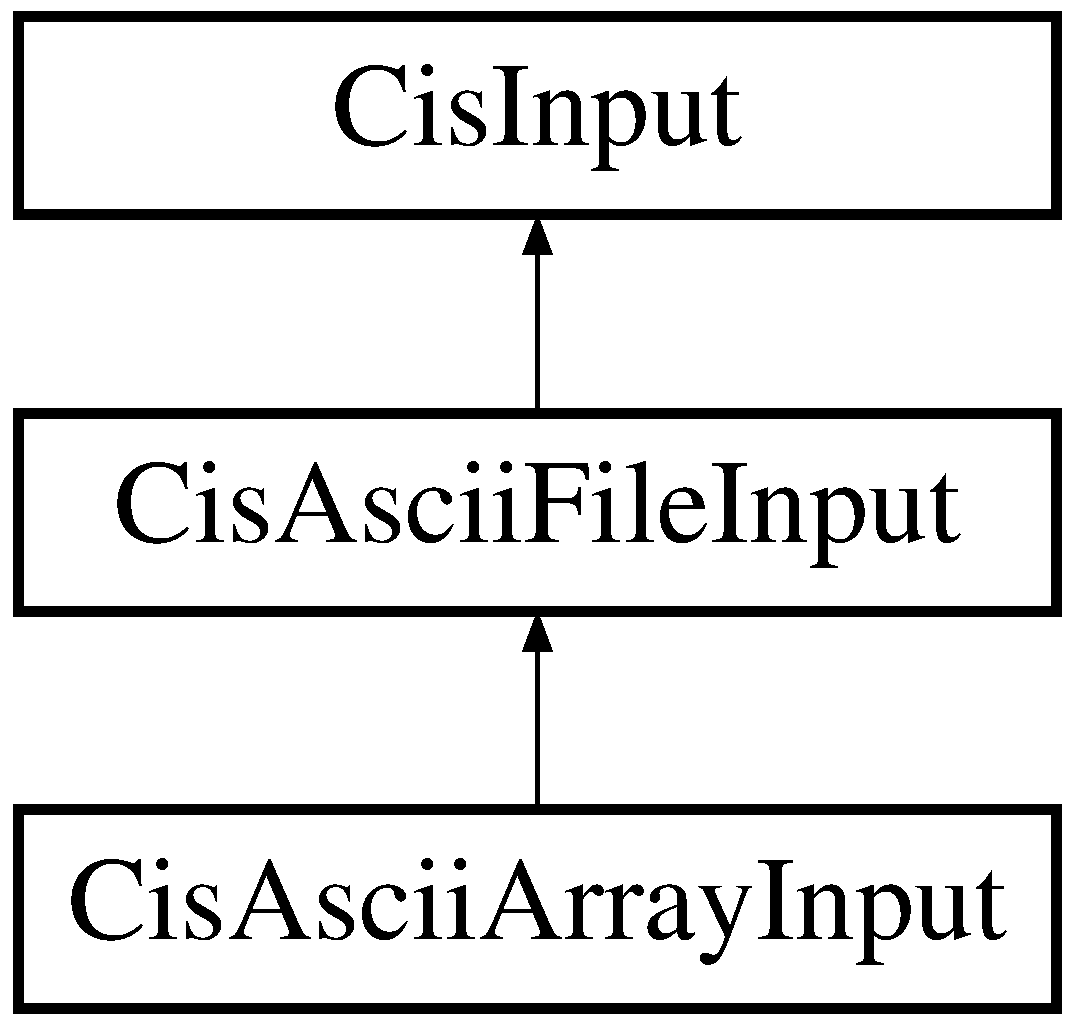
\includegraphics[height=3.000000cm]{classCisAsciiArrayInput}
\end{center}
\end{figure}
\subsection*{Public Member Functions}
\begin{DoxyCompactItemize}
\item 
\mbox{\hyperlink{classCisAsciiArrayInput_a5b93411bc0df794c6f6a3189d2e02289}{Cis\+Ascii\+Array\+Input}} (const char $\ast$name)
\begin{DoxyCompactList}\small\item\em Constructor for \mbox{\hyperlink{classCisAsciiArrayInput}{Cis\+Ascii\+Array\+Input}}. Due to issues with the C++ version of vsscanf, flags and precision indicators for floating point format specifiers (e.\+g. e, f), must be removed so that table input can be properly parsed. \end{DoxyCompactList}\end{DoxyCompactItemize}


\subsection{Detailed Description}
C++ interface to cis\+Ascii\+Table\+Input\+\_\+t functionality for arrays. 

The \mbox{\hyperlink{classCisAsciiArrayInput}{Cis\+Ascii\+Array\+Input}} class is a basic wrapper around the C cis\+Ascii\+Table\+Input\+\_\+t structure and associated functions from the \mbox{\hyperlink{CisInterface_8h_source}{Cis\+Interface.\+h}} header. It provides the user with C++ style access to basic A\+S\+C\+II table input operations. 

\subsection{Constructor \& Destructor Documentation}
\mbox{\Hypertarget{classCisAsciiArrayInput_a5b93411bc0df794c6f6a3189d2e02289}\label{classCisAsciiArrayInput_a5b93411bc0df794c6f6a3189d2e02289}} 
\index{Cis\+Ascii\+Array\+Input@{Cis\+Ascii\+Array\+Input}!Cis\+Ascii\+Array\+Input@{Cis\+Ascii\+Array\+Input}}
\index{Cis\+Ascii\+Array\+Input@{Cis\+Ascii\+Array\+Input}!Cis\+Ascii\+Array\+Input@{Cis\+Ascii\+Array\+Input}}
\subsubsection{\texorpdfstring{Cis\+Ascii\+Array\+Input()}{CisAsciiArrayInput()}}
{\footnotesize\ttfamily Cis\+Ascii\+Array\+Input\+::\+Cis\+Ascii\+Array\+Input (\begin{DoxyParamCaption}\item[{const char $\ast$}]{name }\end{DoxyParamCaption})\hspace{0.3cm}{\ttfamily [inline]}}



Constructor for \mbox{\hyperlink{classCisAsciiArrayInput}{Cis\+Ascii\+Array\+Input}}. Due to issues with the C++ version of vsscanf, flags and precision indicators for floating point format specifiers (e.\+g. e, f), must be removed so that table input can be properly parsed. 


\begin{DoxyParams}[1]{Parameters}
\mbox{\tt in}  & {\em name} & constant character pointer to the name of an input channel. \\
\hline
\end{DoxyParams}


The documentation for this class was generated from the following file\+:\begin{DoxyCompactItemize}
\item 
/root/cis\+\_\+interface/cis\+\_\+interface/cis\+\_\+interface/interface/Cis\+Interface.\+hpp\end{DoxyCompactItemize}

\hypertarget{classCisAsciiArrayInput__local}{}\section{Cis\+Ascii\+Array\+Input\+\_\+local Class Reference}
\label{classCisAsciiArrayInput__local}\index{Cis\+Ascii\+Array\+Input\+\_\+local@{Cis\+Ascii\+Array\+Input\+\_\+local}}


C++ interface to cis\+Ascii\+Table\+Input\+\_\+t functionality for local files as arrays.  




{\ttfamily \#include $<$Cis\+Interface.\+hpp$>$}

Inheritance diagram for Cis\+Ascii\+Array\+Input\+\_\+local\+:\begin{figure}[H]
\begin{center}
\leavevmode
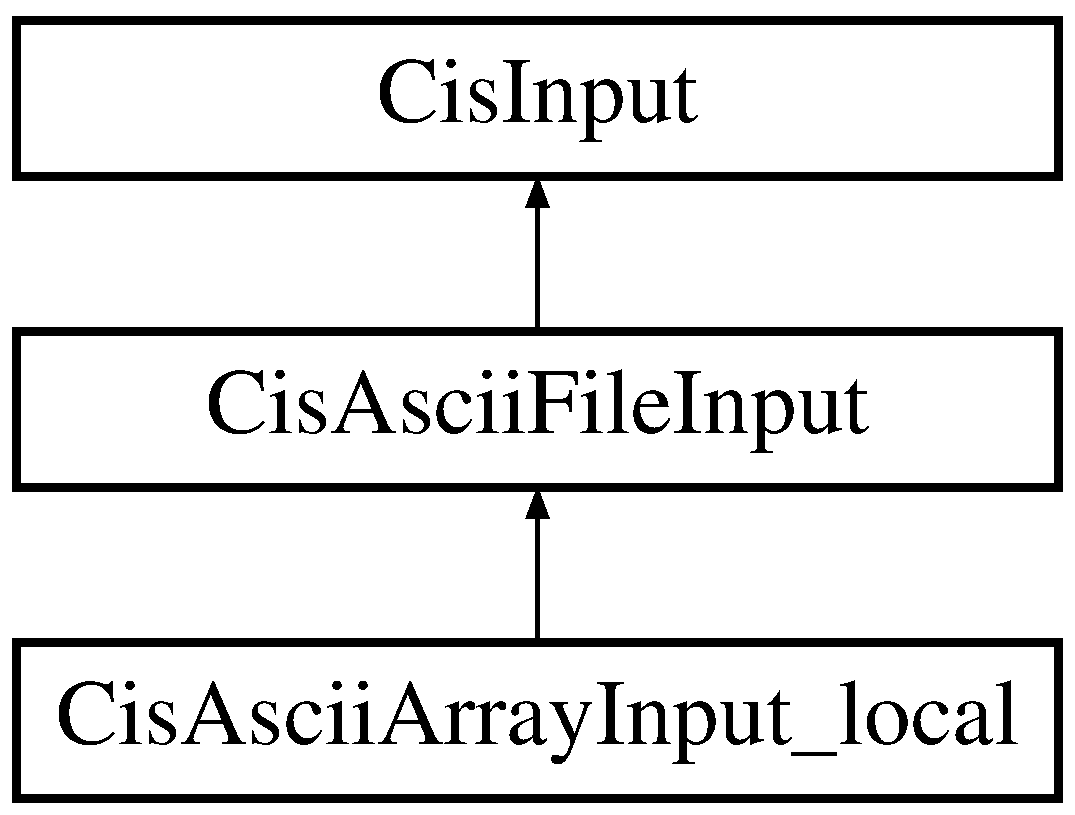
\includegraphics[height=3.000000cm]{classCisAsciiArrayInput__local}
\end{center}
\end{figure}
\subsection*{Public Member Functions}
\begin{DoxyCompactItemize}
\item 
\mbox{\hyperlink{classCisAsciiArrayInput__local_ab1a315749639f0edd562184bcdb34d42}{Cis\+Ascii\+Array\+Input\+\_\+local}} (const char $\ast$name)
\begin{DoxyCompactList}\small\item\em Constructor for \mbox{\hyperlink{classCisAsciiArrayInput__local}{Cis\+Ascii\+Array\+Input\+\_\+local}}. Due to issues with the C++ version of vsscanf, flags and precision indicators for floating point format specifiers (e.\+g. e, f), must be removed so that table input can be properly parsed. \end{DoxyCompactList}\end{DoxyCompactItemize}


\subsection{Detailed Description}
C++ interface to cis\+Ascii\+Table\+Input\+\_\+t functionality for local files as arrays. 

The \mbox{\hyperlink{classCisAsciiArrayInput}{Cis\+Ascii\+Array\+Input}} class is a basic wrapper around the C cis\+Ascii\+Table\+Input\+\_\+t structure and associated functions from the \mbox{\hyperlink{CisInterface_8h_source}{Cis\+Interface.\+h}} header. It provides the user with C++ style access to basic A\+S\+C\+II table input operations. 

\subsection{Constructor \& Destructor Documentation}
\mbox{\Hypertarget{classCisAsciiArrayInput__local_ab1a315749639f0edd562184bcdb34d42}\label{classCisAsciiArrayInput__local_ab1a315749639f0edd562184bcdb34d42}} 
\index{Cis\+Ascii\+Array\+Input\+\_\+local@{Cis\+Ascii\+Array\+Input\+\_\+local}!Cis\+Ascii\+Array\+Input\+\_\+local@{Cis\+Ascii\+Array\+Input\+\_\+local}}
\index{Cis\+Ascii\+Array\+Input\+\_\+local@{Cis\+Ascii\+Array\+Input\+\_\+local}!Cis\+Ascii\+Array\+Input\+\_\+local@{Cis\+Ascii\+Array\+Input\+\_\+local}}
\subsubsection{\texorpdfstring{Cis\+Ascii\+Array\+Input\+\_\+local()}{CisAsciiArrayInput\_local()}}
{\footnotesize\ttfamily Cis\+Ascii\+Array\+Input\+\_\+local\+::\+Cis\+Ascii\+Array\+Input\+\_\+local (\begin{DoxyParamCaption}\item[{const char $\ast$}]{name }\end{DoxyParamCaption})\hspace{0.3cm}{\ttfamily [inline]}}



Constructor for \mbox{\hyperlink{classCisAsciiArrayInput__local}{Cis\+Ascii\+Array\+Input\+\_\+local}}. Due to issues with the C++ version of vsscanf, flags and precision indicators for floating point format specifiers (e.\+g. e, f), must be removed so that table input can be properly parsed. 


\begin{DoxyParams}[1]{Parameters}
\mbox{\tt in}  & {\em name} & constant character pointer to path of local table. \\
\hline
\end{DoxyParams}


The documentation for this class was generated from the following file\+:\begin{DoxyCompactItemize}
\item 
/root/cis\+\_\+interface/cis\+\_\+interface/cis\+\_\+interface/interface/Cis\+Interface.\+hpp\end{DoxyCompactItemize}

\hypertarget{classCisAsciiArrayOutput}{}\section{Cis\+Ascii\+Array\+Output Class Reference}
\label{classCisAsciiArrayOutput}\index{Cis\+Ascii\+Array\+Output@{Cis\+Ascii\+Array\+Output}}


C++ interface to cis\+Ascii\+Table\+Output\+\_\+t functionality with arrays.  




{\ttfamily \#include $<$Cis\+Interface.\+hpp$>$}

Inheritance diagram for Cis\+Ascii\+Array\+Output\+:\begin{figure}[H]
\begin{center}
\leavevmode
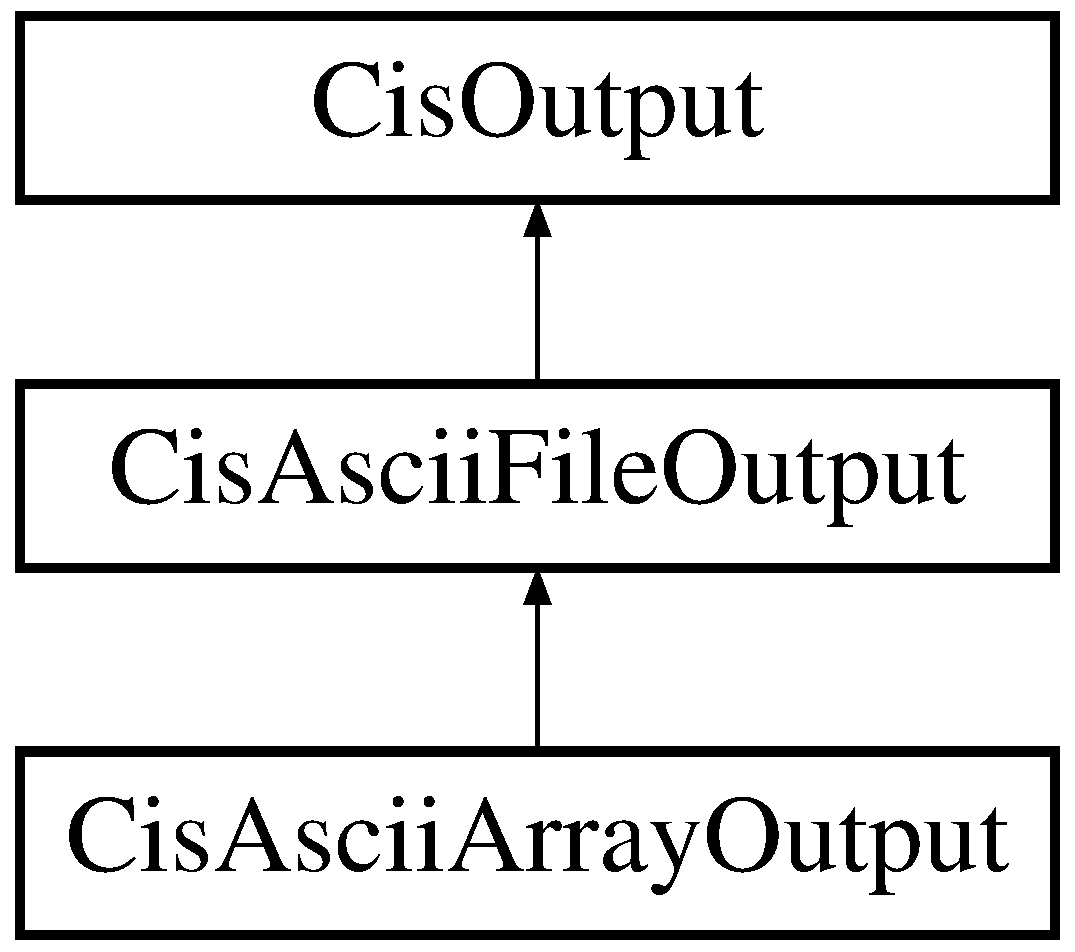
\includegraphics[height=3.000000cm]{classCisAsciiArrayOutput}
\end{center}
\end{figure}
\subsection*{Public Member Functions}
\begin{DoxyCompactItemize}
\item 
\mbox{\hyperlink{classCisAsciiArrayOutput_a3a4e19e80478aa1748f4074d72d3932a}{Cis\+Ascii\+Array\+Output}} (const char $\ast$name, const char $\ast$format\+\_\+str)
\begin{DoxyCompactList}\small\item\em Constructor for \mbox{\hyperlink{classCisAsciiArrayOutput}{Cis\+Ascii\+Array\+Output}}. \end{DoxyCompactList}\end{DoxyCompactItemize}


\subsection{Detailed Description}
C++ interface to cis\+Ascii\+Table\+Output\+\_\+t functionality with arrays. 

The \mbox{\hyperlink{classCisAsciiArrayOutput}{Cis\+Ascii\+Array\+Output}} class is a basic wrapper around the C cis\+Ascii\+Table\+Output\+\_\+t structure and associated functions from the \mbox{\hyperlink{CisInterface_8h_source}{Cis\+Interface.\+h}} header. It provides the user with C++ style access to basic A\+S\+C\+II table output operations. 

\subsection{Constructor \& Destructor Documentation}
\mbox{\Hypertarget{classCisAsciiArrayOutput_a3a4e19e80478aa1748f4074d72d3932a}\label{classCisAsciiArrayOutput_a3a4e19e80478aa1748f4074d72d3932a}} 
\index{Cis\+Ascii\+Array\+Output@{Cis\+Ascii\+Array\+Output}!Cis\+Ascii\+Array\+Output@{Cis\+Ascii\+Array\+Output}}
\index{Cis\+Ascii\+Array\+Output@{Cis\+Ascii\+Array\+Output}!Cis\+Ascii\+Array\+Output@{Cis\+Ascii\+Array\+Output}}
\subsubsection{\texorpdfstring{Cis\+Ascii\+Array\+Output()}{CisAsciiArrayOutput()}}
{\footnotesize\ttfamily Cis\+Ascii\+Array\+Output\+::\+Cis\+Ascii\+Array\+Output (\begin{DoxyParamCaption}\item[{const char $\ast$}]{name,  }\item[{const char $\ast$}]{format\+\_\+str }\end{DoxyParamCaption})\hspace{0.3cm}{\ttfamily [inline]}}



Constructor for \mbox{\hyperlink{classCisAsciiArrayOutput}{Cis\+Ascii\+Array\+Output}}. 


\begin{DoxyParams}[1]{Parameters}
\mbox{\tt in}  & {\em name} & constant character pointer to the name of an output channel. \\
\hline
\mbox{\tt in}  & {\em format\+\_\+str} & character pointer to format string that should be used to format arrays into a table. \\
\hline
\end{DoxyParams}


The documentation for this class was generated from the following file\+:\begin{DoxyCompactItemize}
\item 
/root/cis\+\_\+interface/cis\+\_\+interface/cis\+\_\+interface/interface/Cis\+Interface.\+hpp\end{DoxyCompactItemize}

\hypertarget{classCisAsciiArrayOutput__local}{}\section{Cis\+Ascii\+Array\+Output\+\_\+local Class Reference}
\label{classCisAsciiArrayOutput__local}\index{Cis\+Ascii\+Array\+Output\+\_\+local@{Cis\+Ascii\+Array\+Output\+\_\+local}}


C++ interface to cis\+Ascii\+Table\+Output\+\_\+t functionality for local files.  




{\ttfamily \#include $<$Cis\+Interface.\+hpp$>$}

Inheritance diagram for Cis\+Ascii\+Array\+Output\+\_\+local\+:\begin{figure}[H]
\begin{center}
\leavevmode
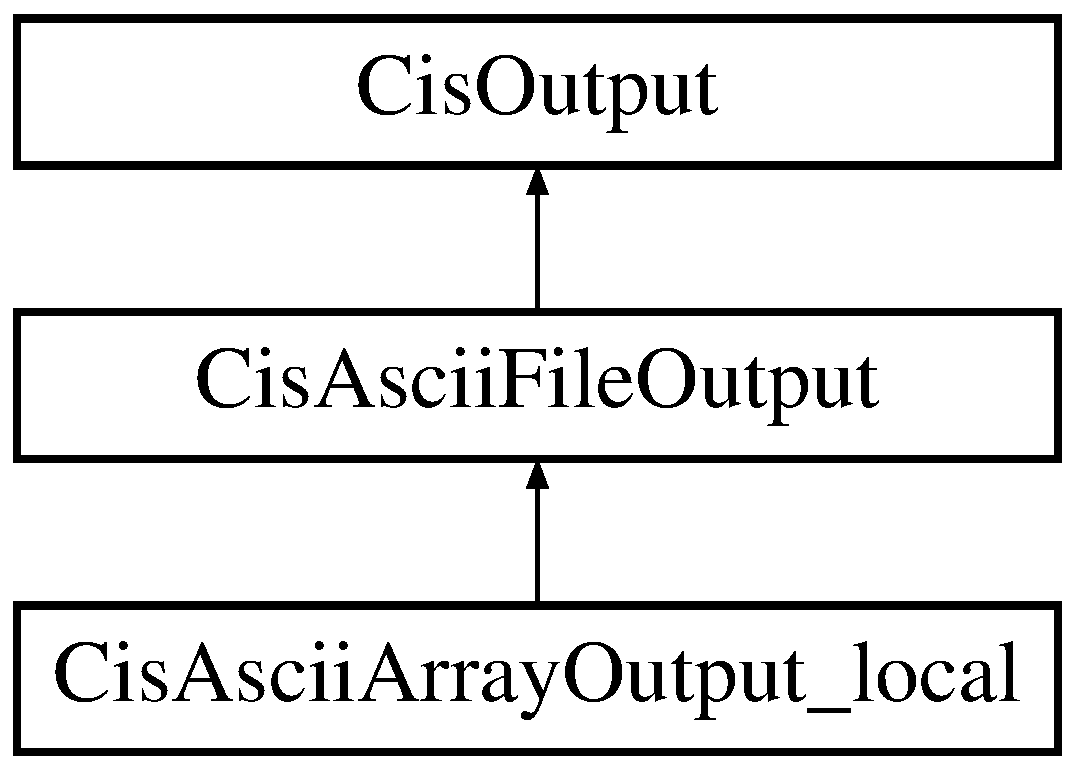
\includegraphics[height=3.000000cm]{classCisAsciiArrayOutput__local}
\end{center}
\end{figure}
\subsection*{Public Member Functions}
\begin{DoxyCompactItemize}
\item 
\mbox{\hyperlink{classCisAsciiArrayOutput__local_a65fa28278be3cf10be0e1a4882f2327f}{Cis\+Ascii\+Array\+Output\+\_\+local}} (const char $\ast$name, const char $\ast$format\+\_\+str)
\begin{DoxyCompactList}\small\item\em Constructor for \mbox{\hyperlink{classCisAsciiArrayOutput}{Cis\+Ascii\+Array\+Output}} for local files. \end{DoxyCompactList}\end{DoxyCompactItemize}


\subsection{Detailed Description}
C++ interface to cis\+Ascii\+Table\+Output\+\_\+t functionality for local files. 

The \mbox{\hyperlink{classCisAsciiArrayOutput}{Cis\+Ascii\+Array\+Output}} class is a basic wrapper around the C cis\+Ascii\+Table\+Output\+\_\+t structure and associated functions from the \mbox{\hyperlink{CisInterface_8h_source}{Cis\+Interface.\+h}} header. It provides the user with C++ style access to basic A\+S\+C\+II table output operations. 

\subsection{Constructor \& Destructor Documentation}
\mbox{\Hypertarget{classCisAsciiArrayOutput__local_a65fa28278be3cf10be0e1a4882f2327f}\label{classCisAsciiArrayOutput__local_a65fa28278be3cf10be0e1a4882f2327f}} 
\index{Cis\+Ascii\+Array\+Output\+\_\+local@{Cis\+Ascii\+Array\+Output\+\_\+local}!Cis\+Ascii\+Array\+Output\+\_\+local@{Cis\+Ascii\+Array\+Output\+\_\+local}}
\index{Cis\+Ascii\+Array\+Output\+\_\+local@{Cis\+Ascii\+Array\+Output\+\_\+local}!Cis\+Ascii\+Array\+Output\+\_\+local@{Cis\+Ascii\+Array\+Output\+\_\+local}}
\subsubsection{\texorpdfstring{Cis\+Ascii\+Array\+Output\+\_\+local()}{CisAsciiArrayOutput\_local()}}
{\footnotesize\ttfamily Cis\+Ascii\+Array\+Output\+\_\+local\+::\+Cis\+Ascii\+Array\+Output\+\_\+local (\begin{DoxyParamCaption}\item[{const char $\ast$}]{name,  }\item[{const char $\ast$}]{format\+\_\+str }\end{DoxyParamCaption})\hspace{0.3cm}{\ttfamily [inline]}}



Constructor for \mbox{\hyperlink{classCisAsciiArrayOutput}{Cis\+Ascii\+Array\+Output}} for local files. 


\begin{DoxyParams}[1]{Parameters}
\mbox{\tt in}  & {\em name} & constant character pointer to path of local table. \\
\hline
\mbox{\tt in}  & {\em format\+\_\+str} & character pointer to format string that should be used to format arrays into table columns. \\
\hline
\end{DoxyParams}


The documentation for this class was generated from the following file\+:\begin{DoxyCompactItemize}
\item 
/root/cis\+\_\+interface/cis\+\_\+interface/cis\+\_\+interface/interface/Cis\+Interface.\+hpp\end{DoxyCompactItemize}

\hypertarget{classCisAsciiFileInput}{}\section{Cis\+Ascii\+File\+Input Class Reference}
\label{classCisAsciiFileInput}\index{Cis\+Ascii\+File\+Input@{Cis\+Ascii\+File\+Input}}


C++ interface to cis\+Ascii\+File\+Input\+\_\+t functionality. The \mbox{\hyperlink{classCisAsciiFileInput}{Cis\+Ascii\+File\+Input}} class is a basic wrapper around the C cis\+Ascii\+File\+Input\+\_\+t structure and associated functions from the \mbox{\hyperlink{CisInterface_8h_source}{Cis\+Interface.\+h}} header. It provides the user with C++ style access to basic A\+S\+C\+II file input operations.  




{\ttfamily \#include $<$Cis\+Interface.\+hpp$>$}

Inheritance diagram for Cis\+Ascii\+File\+Input\+:\begin{figure}[H]
\begin{center}
\leavevmode
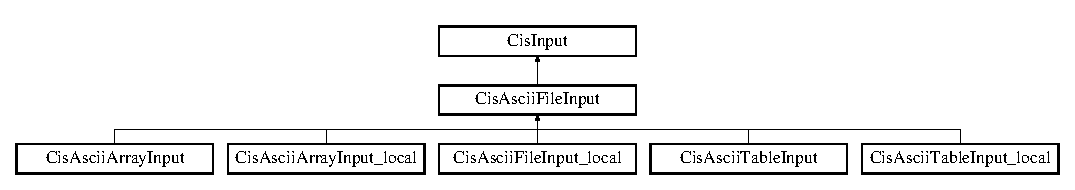
\includegraphics[height=2.100000cm]{classCisAsciiFileInput}
\end{center}
\end{figure}
\subsection*{Public Member Functions}
\begin{DoxyCompactItemize}
\item 
\mbox{\hyperlink{classCisAsciiFileInput_aac31cfe291fe9b5f4dc16bb78a123e8c}{Cis\+Ascii\+File\+Input}} (const char $\ast$name)
\begin{DoxyCompactList}\small\item\em Constructor for \mbox{\hyperlink{classCisAsciiFileInput}{Cis\+Ascii\+File\+Input}}. \end{DoxyCompactList}\item 
\mbox{\Hypertarget{classCisAsciiFileInput_a7bee575f759ecb42dbe4d525638d5bc1}\label{classCisAsciiFileInput_a7bee575f759ecb42dbe4d525638d5bc1}} 
\mbox{\hyperlink{classCisAsciiFileInput_a7bee575f759ecb42dbe4d525638d5bc1}{Cis\+Ascii\+File\+Input}} (cis\+Input\+\_\+t x)
\begin{DoxyCompactList}\small\item\em Empty constructor for inheritance. \end{DoxyCompactList}\item 
int \mbox{\hyperlink{classCisAsciiFileInput_a4509672e282e82990974104a811c1605}{recv\+\_\+line}} (char $\ast$line, const size\+\_\+t n)
\begin{DoxyCompactList}\small\item\em Receive a single line from an associated file or queue. See af\+\_\+recv\+\_\+line in \mbox{\hyperlink{CisInterface_8h_source}{Cis\+Interface.\+h}} for details. \end{DoxyCompactList}\end{DoxyCompactItemize}


\subsection{Detailed Description}
C++ interface to cis\+Ascii\+File\+Input\+\_\+t functionality. The \mbox{\hyperlink{classCisAsciiFileInput}{Cis\+Ascii\+File\+Input}} class is a basic wrapper around the C cis\+Ascii\+File\+Input\+\_\+t structure and associated functions from the \mbox{\hyperlink{CisInterface_8h_source}{Cis\+Interface.\+h}} header. It provides the user with C++ style access to basic A\+S\+C\+II file input operations. 

\subsection{Constructor \& Destructor Documentation}
\mbox{\Hypertarget{classCisAsciiFileInput_aac31cfe291fe9b5f4dc16bb78a123e8c}\label{classCisAsciiFileInput_aac31cfe291fe9b5f4dc16bb78a123e8c}} 
\index{Cis\+Ascii\+File\+Input@{Cis\+Ascii\+File\+Input}!Cis\+Ascii\+File\+Input@{Cis\+Ascii\+File\+Input}}
\index{Cis\+Ascii\+File\+Input@{Cis\+Ascii\+File\+Input}!Cis\+Ascii\+File\+Input@{Cis\+Ascii\+File\+Input}}
\subsubsection{\texorpdfstring{Cis\+Ascii\+File\+Input()}{CisAsciiFileInput()}}
{\footnotesize\ttfamily Cis\+Ascii\+File\+Input\+::\+Cis\+Ascii\+File\+Input (\begin{DoxyParamCaption}\item[{const char $\ast$}]{name }\end{DoxyParamCaption})\hspace{0.3cm}{\ttfamily [inline]}}



Constructor for \mbox{\hyperlink{classCisAsciiFileInput}{Cis\+Ascii\+File\+Input}}. 


\begin{DoxyParams}[1]{Parameters}
\mbox{\tt in}  & {\em name} & constant character pointer to the name of an input channel. \\
\hline
\end{DoxyParams}


\subsection{Member Function Documentation}
\mbox{\Hypertarget{classCisAsciiFileInput_a4509672e282e82990974104a811c1605}\label{classCisAsciiFileInput_a4509672e282e82990974104a811c1605}} 
\index{Cis\+Ascii\+File\+Input@{Cis\+Ascii\+File\+Input}!recv\+\_\+line@{recv\+\_\+line}}
\index{recv\+\_\+line@{recv\+\_\+line}!Cis\+Ascii\+File\+Input@{Cis\+Ascii\+File\+Input}}
\subsubsection{\texorpdfstring{recv\+\_\+line()}{recv\_line()}}
{\footnotesize\ttfamily int Cis\+Ascii\+File\+Input\+::recv\+\_\+line (\begin{DoxyParamCaption}\item[{char $\ast$}]{line,  }\item[{const size\+\_\+t}]{n }\end{DoxyParamCaption})\hspace{0.3cm}{\ttfamily [inline]}}



Receive a single line from an associated file or queue. See af\+\_\+recv\+\_\+line in \mbox{\hyperlink{CisInterface_8h_source}{Cis\+Interface.\+h}} for details. 


\begin{DoxyParams}[1]{Parameters}
\mbox{\tt out}  & {\em line} & character pointer to allocate memory where the received line should be stored. \\
\hline
\mbox{\tt in}  & {\em n} & size\+\_\+t Size of the allocated memory block in bytes. \\
\hline
\end{DoxyParams}
\begin{DoxyReturn}{Returns}
int Number of bytes read/received. Negative values indicate that there was either an error or the E\+OF message was received. 
\end{DoxyReturn}


The documentation for this class was generated from the following file\+:\begin{DoxyCompactItemize}
\item 
/root/cis\+\_\+interface/cis\+\_\+interface/cis\+\_\+interface/interface/Cis\+Interface.\+hpp\end{DoxyCompactItemize}

\hypertarget{classCisAsciiFileInput__local}{}\section{Cis\+Ascii\+File\+Input\+\_\+local Class Reference}
\label{classCisAsciiFileInput__local}\index{Cis\+Ascii\+File\+Input\+\_\+local@{Cis\+Ascii\+File\+Input\+\_\+local}}


C++ interface to cis\+Ascii\+File\+Input\+\_\+t functionality for local files. The \mbox{\hyperlink{classCisAsciiFileInput__local}{Cis\+Ascii\+File\+Input\+\_\+local}} class is a basic wrapper around the C cis\+Ascii\+File\+Input\+\_\+t structure and associated functions from the \mbox{\hyperlink{CisInterface_8h_source}{Cis\+Interface.\+h}} header. It provides the user with C++ style access to basic A\+S\+C\+II file input operations.  




{\ttfamily \#include $<$Cis\+Interface.\+hpp$>$}

Inheritance diagram for Cis\+Ascii\+File\+Input\+\_\+local\+:\begin{figure}[H]
\begin{center}
\leavevmode
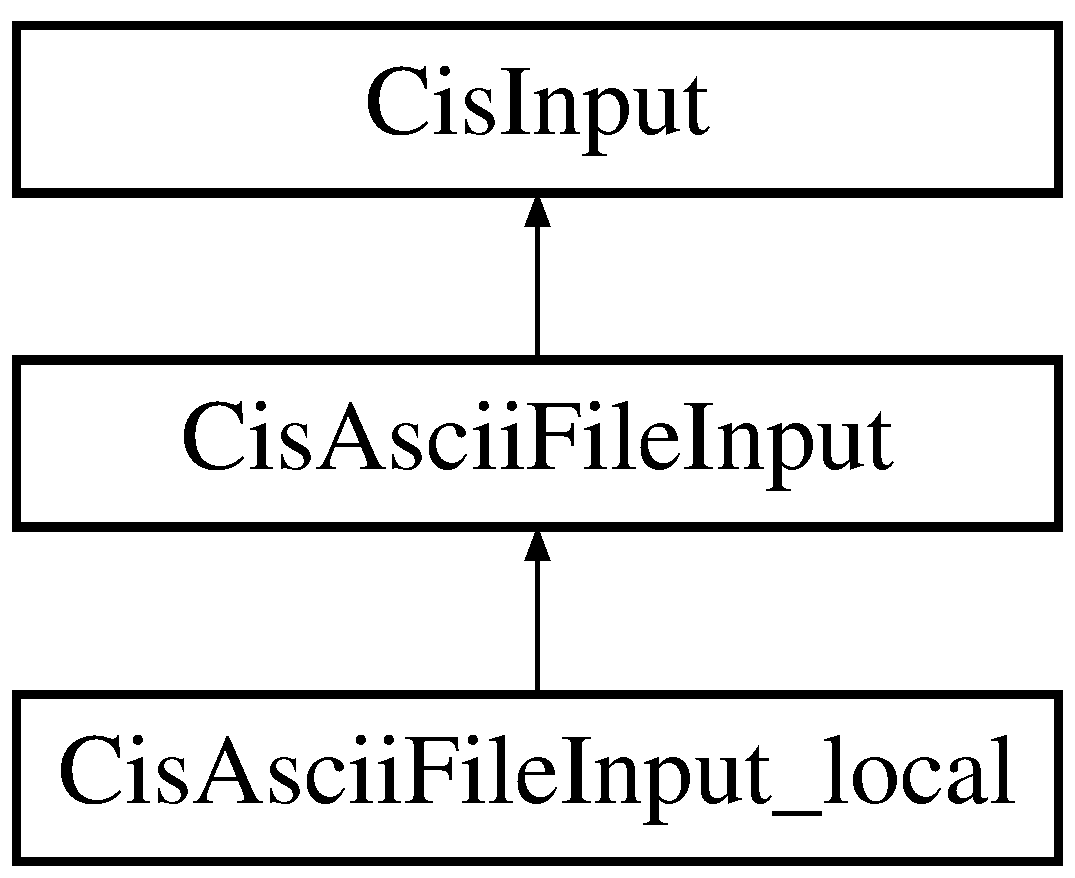
\includegraphics[height=3.000000cm]{classCisAsciiFileInput__local}
\end{center}
\end{figure}
\subsection*{Public Member Functions}
\begin{DoxyCompactItemize}
\item 
\mbox{\hyperlink{classCisAsciiFileInput__local_a6a503a34514e6c0bd5ba6429393b2629}{Cis\+Ascii\+File\+Input\+\_\+local}} (const char $\ast$name)
\begin{DoxyCompactList}\small\item\em Constructor for \mbox{\hyperlink{classCisAsciiFileInput__local}{Cis\+Ascii\+File\+Input\+\_\+local}}. \end{DoxyCompactList}\end{DoxyCompactItemize}


\subsection{Detailed Description}
C++ interface to cis\+Ascii\+File\+Input\+\_\+t functionality for local files. The \mbox{\hyperlink{classCisAsciiFileInput__local}{Cis\+Ascii\+File\+Input\+\_\+local}} class is a basic wrapper around the C cis\+Ascii\+File\+Input\+\_\+t structure and associated functions from the \mbox{\hyperlink{CisInterface_8h_source}{Cis\+Interface.\+h}} header. It provides the user with C++ style access to basic A\+S\+C\+II file input operations. 

\subsection{Constructor \& Destructor Documentation}
\mbox{\Hypertarget{classCisAsciiFileInput__local_a6a503a34514e6c0bd5ba6429393b2629}\label{classCisAsciiFileInput__local_a6a503a34514e6c0bd5ba6429393b2629}} 
\index{Cis\+Ascii\+File\+Input\+\_\+local@{Cis\+Ascii\+File\+Input\+\_\+local}!Cis\+Ascii\+File\+Input\+\_\+local@{Cis\+Ascii\+File\+Input\+\_\+local}}
\index{Cis\+Ascii\+File\+Input\+\_\+local@{Cis\+Ascii\+File\+Input\+\_\+local}!Cis\+Ascii\+File\+Input\+\_\+local@{Cis\+Ascii\+File\+Input\+\_\+local}}
\subsubsection{\texorpdfstring{Cis\+Ascii\+File\+Input\+\_\+local()}{CisAsciiFileInput\_local()}}
{\footnotesize\ttfamily Cis\+Ascii\+File\+Input\+\_\+local\+::\+Cis\+Ascii\+File\+Input\+\_\+local (\begin{DoxyParamCaption}\item[{const char $\ast$}]{name }\end{DoxyParamCaption})\hspace{0.3cm}{\ttfamily [inline]}}



Constructor for \mbox{\hyperlink{classCisAsciiFileInput__local}{Cis\+Ascii\+File\+Input\+\_\+local}}. 


\begin{DoxyParams}[1]{Parameters}
\mbox{\tt in}  & {\em name} & constant character pointer to path of local file. \\
\hline
\end{DoxyParams}


The documentation for this class was generated from the following file\+:\begin{DoxyCompactItemize}
\item 
/root/cis\+\_\+interface/cis\+\_\+interface/cis\+\_\+interface/interface/Cis\+Interface.\+hpp\end{DoxyCompactItemize}

\hypertarget{classCisAsciiFileOutput}{}\section{Cis\+Ascii\+File\+Output Class Reference}
\label{classCisAsciiFileOutput}\index{Cis\+Ascii\+File\+Output@{Cis\+Ascii\+File\+Output}}


C++ interface to cis\+Ascii\+File\+Output\+\_\+t functionality. The \mbox{\hyperlink{classCisAsciiFileOutput}{Cis\+Ascii\+File\+Output}} class is a basic wrapper around the C cis\+Ascii\+File\+Output\+\_\+t structure and associated functions from the \mbox{\hyperlink{CisInterface_8h_source}{Cis\+Interface.\+h}} header. It provides the user with C++ style access to basic A\+S\+C\+II file output operations.  




{\ttfamily \#include $<$Cis\+Interface.\+hpp$>$}

Inheritance diagram for Cis\+Ascii\+File\+Output\+:\begin{figure}[H]
\begin{center}
\leavevmode
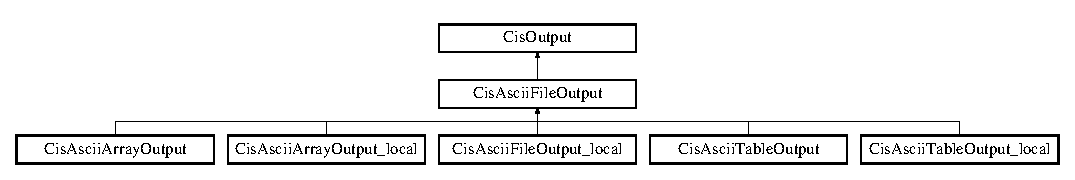
\includegraphics[height=1.976471cm]{classCisAsciiFileOutput}
\end{center}
\end{figure}
\subsection*{Public Member Functions}
\begin{DoxyCompactItemize}
\item 
\mbox{\hyperlink{classCisAsciiFileOutput_ab17524610ace98b485e02932ba3468af}{Cis\+Ascii\+File\+Output}} (const char $\ast$name)
\begin{DoxyCompactList}\small\item\em Constructor for \mbox{\hyperlink{classCisAsciiFileOutput}{Cis\+Ascii\+File\+Output}}. \end{DoxyCompactList}\item 
\mbox{\Hypertarget{classCisAsciiFileOutput_a123f97ab25f1930bc4930e468de1bf05}\label{classCisAsciiFileOutput_a123f97ab25f1930bc4930e468de1bf05}} 
\mbox{\hyperlink{classCisAsciiFileOutput_a123f97ab25f1930bc4930e468de1bf05}{Cis\+Ascii\+File\+Output}} (cis\+Output\+\_\+t x)
\begin{DoxyCompactList}\small\item\em Empty constructor for inheritance. \end{DoxyCompactList}\item 
int \mbox{\hyperlink{classCisAsciiFileOutput_a8863d020f0cc7c4690fa0877358eae6d}{send\+\_\+line}} (const char $\ast$line)
\begin{DoxyCompactList}\small\item\em Send a single line to a file or queue. \end{DoxyCompactList}\end{DoxyCompactItemize}


\subsection{Detailed Description}
C++ interface to cis\+Ascii\+File\+Output\+\_\+t functionality. The \mbox{\hyperlink{classCisAsciiFileOutput}{Cis\+Ascii\+File\+Output}} class is a basic wrapper around the C cis\+Ascii\+File\+Output\+\_\+t structure and associated functions from the \mbox{\hyperlink{CisInterface_8h_source}{Cis\+Interface.\+h}} header. It provides the user with C++ style access to basic A\+S\+C\+II file output operations. 

\subsection{Constructor \& Destructor Documentation}
\mbox{\Hypertarget{classCisAsciiFileOutput_ab17524610ace98b485e02932ba3468af}\label{classCisAsciiFileOutput_ab17524610ace98b485e02932ba3468af}} 
\index{Cis\+Ascii\+File\+Output@{Cis\+Ascii\+File\+Output}!Cis\+Ascii\+File\+Output@{Cis\+Ascii\+File\+Output}}
\index{Cis\+Ascii\+File\+Output@{Cis\+Ascii\+File\+Output}!Cis\+Ascii\+File\+Output@{Cis\+Ascii\+File\+Output}}
\subsubsection{\texorpdfstring{Cis\+Ascii\+File\+Output()}{CisAsciiFileOutput()}}
{\footnotesize\ttfamily Cis\+Ascii\+File\+Output\+::\+Cis\+Ascii\+File\+Output (\begin{DoxyParamCaption}\item[{const char $\ast$}]{name }\end{DoxyParamCaption})\hspace{0.3cm}{\ttfamily [inline]}}



Constructor for \mbox{\hyperlink{classCisAsciiFileOutput}{Cis\+Ascii\+File\+Output}}. 


\begin{DoxyParams}[1]{Parameters}
\mbox{\tt in}  & {\em name} & constant character pointer to the name of an output channel. \\
\hline
\end{DoxyParams}


\subsection{Member Function Documentation}
\mbox{\Hypertarget{classCisAsciiFileOutput_a8863d020f0cc7c4690fa0877358eae6d}\label{classCisAsciiFileOutput_a8863d020f0cc7c4690fa0877358eae6d}} 
\index{Cis\+Ascii\+File\+Output@{Cis\+Ascii\+File\+Output}!send\+\_\+line@{send\+\_\+line}}
\index{send\+\_\+line@{send\+\_\+line}!Cis\+Ascii\+File\+Output@{Cis\+Ascii\+File\+Output}}
\subsubsection{\texorpdfstring{send\+\_\+line()}{send\_line()}}
{\footnotesize\ttfamily int Cis\+Ascii\+File\+Output\+::send\+\_\+line (\begin{DoxyParamCaption}\item[{const char $\ast$}]{line }\end{DoxyParamCaption})\hspace{0.3cm}{\ttfamily [inline]}}



Send a single line to a file or queue. 


\begin{DoxyParams}[1]{Parameters}
\mbox{\tt in}  & {\em line} & character pointer to line that should be sent. \\
\hline
\end{DoxyParams}
\begin{DoxyReturn}{Returns}
int 0 if send was succesfull. All other values indicate errors. 
\end{DoxyReturn}


The documentation for this class was generated from the following file\+:\begin{DoxyCompactItemize}
\item 
/root/cis\+\_\+interface/cis\+\_\+interface/cis\+\_\+interface/interface/Cis\+Interface.\+hpp\end{DoxyCompactItemize}

\hypertarget{classCisAsciiFileOutput__local}{}\section{Cis\+Ascii\+File\+Output\+\_\+local Class Reference}
\label{classCisAsciiFileOutput__local}\index{Cis\+Ascii\+File\+Output\+\_\+local@{Cis\+Ascii\+File\+Output\+\_\+local}}


C++ interface to cis\+Ascii\+File\+Output\+\_\+t functionality for local files. The \mbox{\hyperlink{classCisAsciiFileOutput__local}{Cis\+Ascii\+File\+Output\+\_\+local}} class is a basic wrapper around the C cis\+Ascii\+File\+Output\+\_\+t structure and associated functions from the \mbox{\hyperlink{CisInterface_8h_source}{Cis\+Interface.\+h}} header. It provides the user with C++ style access to basic A\+S\+C\+II file output operations.  




{\ttfamily \#include $<$Cis\+Interface.\+hpp$>$}

Inheritance diagram for Cis\+Ascii\+File\+Output\+\_\+local\+:\begin{figure}[H]
\begin{center}
\leavevmode
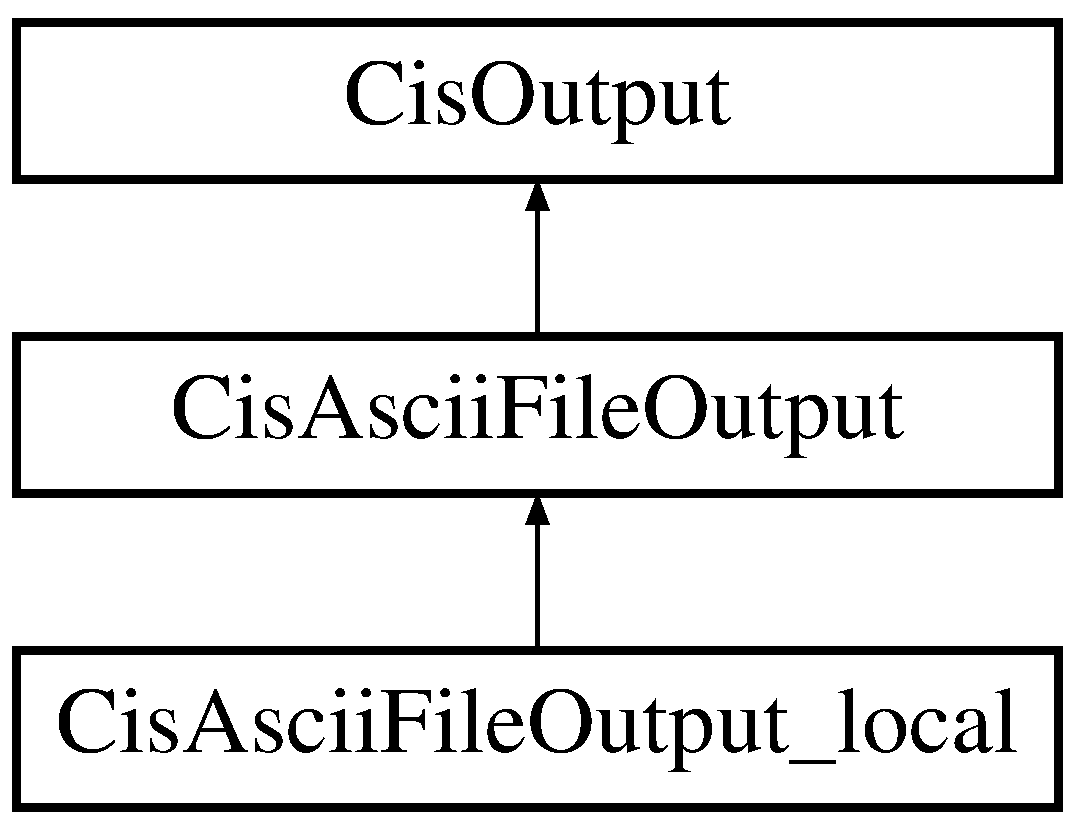
\includegraphics[height=3.000000cm]{classCisAsciiFileOutput__local}
\end{center}
\end{figure}
\subsection*{Public Member Functions}
\begin{DoxyCompactItemize}
\item 
\mbox{\hyperlink{classCisAsciiFileOutput__local_a879ac5cab1e7f7b8625cef59e239db91}{Cis\+Ascii\+File\+Output\+\_\+local}} (const char $\ast$name)
\begin{DoxyCompactList}\small\item\em Constructor for \mbox{\hyperlink{classCisAsciiFileOutput}{Cis\+Ascii\+File\+Output}}. \end{DoxyCompactList}\end{DoxyCompactItemize}


\subsection{Detailed Description}
C++ interface to cis\+Ascii\+File\+Output\+\_\+t functionality for local files. The \mbox{\hyperlink{classCisAsciiFileOutput__local}{Cis\+Ascii\+File\+Output\+\_\+local}} class is a basic wrapper around the C cis\+Ascii\+File\+Output\+\_\+t structure and associated functions from the \mbox{\hyperlink{CisInterface_8h_source}{Cis\+Interface.\+h}} header. It provides the user with C++ style access to basic A\+S\+C\+II file output operations. 

\subsection{Constructor \& Destructor Documentation}
\mbox{\Hypertarget{classCisAsciiFileOutput__local_a879ac5cab1e7f7b8625cef59e239db91}\label{classCisAsciiFileOutput__local_a879ac5cab1e7f7b8625cef59e239db91}} 
\index{Cis\+Ascii\+File\+Output\+\_\+local@{Cis\+Ascii\+File\+Output\+\_\+local}!Cis\+Ascii\+File\+Output\+\_\+local@{Cis\+Ascii\+File\+Output\+\_\+local}}
\index{Cis\+Ascii\+File\+Output\+\_\+local@{Cis\+Ascii\+File\+Output\+\_\+local}!Cis\+Ascii\+File\+Output\+\_\+local@{Cis\+Ascii\+File\+Output\+\_\+local}}
\subsubsection{\texorpdfstring{Cis\+Ascii\+File\+Output\+\_\+local()}{CisAsciiFileOutput\_local()}}
{\footnotesize\ttfamily Cis\+Ascii\+File\+Output\+\_\+local\+::\+Cis\+Ascii\+File\+Output\+\_\+local (\begin{DoxyParamCaption}\item[{const char $\ast$}]{name }\end{DoxyParamCaption})\hspace{0.3cm}{\ttfamily [inline]}}



Constructor for \mbox{\hyperlink{classCisAsciiFileOutput}{Cis\+Ascii\+File\+Output}}. 


\begin{DoxyParams}[1]{Parameters}
\mbox{\tt in}  & {\em name} & constant character pointer to path of local file. \\
\hline
\end{DoxyParams}


The documentation for this class was generated from the following file\+:\begin{DoxyCompactItemize}
\item 
/root/cis\+\_\+interface/cis\+\_\+interface/cis\+\_\+interface/interface/Cis\+Interface.\+hpp\end{DoxyCompactItemize}

\hypertarget{classCisAsciiTableInput}{}\section{Cis\+Ascii\+Table\+Input Class Reference}
\label{classCisAsciiTableInput}\index{Cis\+Ascii\+Table\+Input@{Cis\+Ascii\+Table\+Input}}


C++ interface to cis\+Ascii\+Table\+Input\+\_\+t functionality.  




{\ttfamily \#include $<$Cis\+Interface.\+hpp$>$}

Inheritance diagram for Cis\+Ascii\+Table\+Input\+:\begin{figure}[H]
\begin{center}
\leavevmode
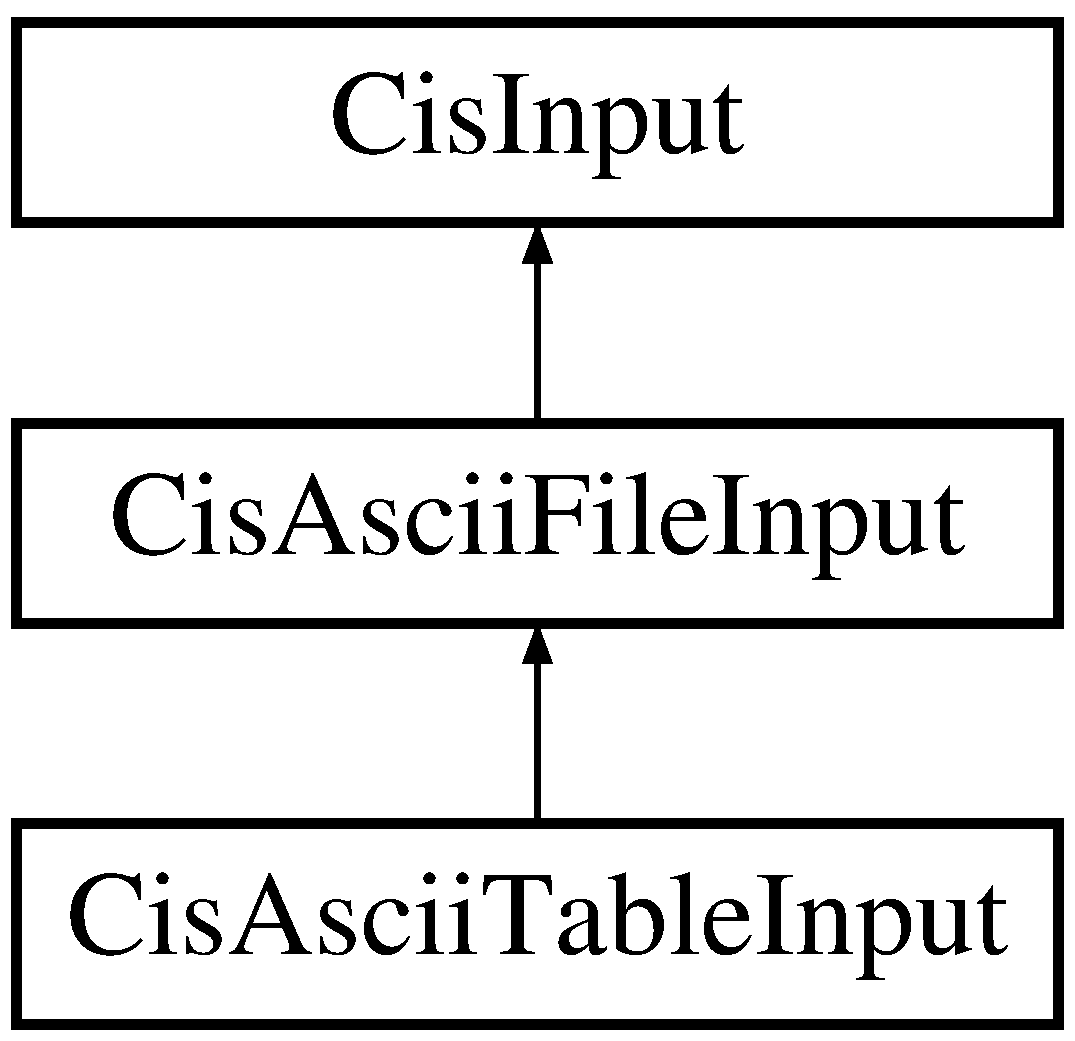
\includegraphics[height=3.000000cm]{classCisAsciiTableInput}
\end{center}
\end{figure}
\subsection*{Public Member Functions}
\begin{DoxyCompactItemize}
\item 
\mbox{\hyperlink{classCisAsciiTableInput_ae87bf636c04e42a7ab745eb164c52b41}{Cis\+Ascii\+Table\+Input}} (const char $\ast$name)
\begin{DoxyCompactList}\small\item\em Constructor for \mbox{\hyperlink{classCisAsciiTableInput}{Cis\+Ascii\+Table\+Input}}. Due to issues with the C++ version of vsscanf, flags and precision indicators for floating point format specifiers (e.\+g. e, f), must be removed so that table input can be properly parsed. \end{DoxyCompactList}\end{DoxyCompactItemize}


\subsection{Detailed Description}
C++ interface to cis\+Ascii\+Table\+Input\+\_\+t functionality. 

The \mbox{\hyperlink{classCisAsciiTableInput}{Cis\+Ascii\+Table\+Input}} class is a basic wrapper around the C cis\+Ascii\+Table\+Input\+\_\+t structure and associated functions from the \mbox{\hyperlink{CisInterface_8h_source}{Cis\+Interface.\+h}} header. It provides the user with C++ style access to basic A\+S\+C\+II table input operations. 

\subsection{Constructor \& Destructor Documentation}
\mbox{\Hypertarget{classCisAsciiTableInput_ae87bf636c04e42a7ab745eb164c52b41}\label{classCisAsciiTableInput_ae87bf636c04e42a7ab745eb164c52b41}} 
\index{Cis\+Ascii\+Table\+Input@{Cis\+Ascii\+Table\+Input}!Cis\+Ascii\+Table\+Input@{Cis\+Ascii\+Table\+Input}}
\index{Cis\+Ascii\+Table\+Input@{Cis\+Ascii\+Table\+Input}!Cis\+Ascii\+Table\+Input@{Cis\+Ascii\+Table\+Input}}
\subsubsection{\texorpdfstring{Cis\+Ascii\+Table\+Input()}{CisAsciiTableInput()}}
{\footnotesize\ttfamily Cis\+Ascii\+Table\+Input\+::\+Cis\+Ascii\+Table\+Input (\begin{DoxyParamCaption}\item[{const char $\ast$}]{name }\end{DoxyParamCaption})\hspace{0.3cm}{\ttfamily [inline]}}



Constructor for \mbox{\hyperlink{classCisAsciiTableInput}{Cis\+Ascii\+Table\+Input}}. Due to issues with the C++ version of vsscanf, flags and precision indicators for floating point format specifiers (e.\+g. e, f), must be removed so that table input can be properly parsed. 


\begin{DoxyParams}[1]{Parameters}
\mbox{\tt in}  & {\em name} & constant character pointer to the name of an input channel. \\
\hline
\end{DoxyParams}


The documentation for this class was generated from the following file\+:\begin{DoxyCompactItemize}
\item 
/root/cis\+\_\+interface/cis\+\_\+interface/cis\+\_\+interface/interface/Cis\+Interface.\+hpp\end{DoxyCompactItemize}

\hypertarget{classCisAsciiTableInput__local}{}\section{Cis\+Ascii\+Table\+Input\+\_\+local Class Reference}
\label{classCisAsciiTableInput__local}\index{Cis\+Ascii\+Table\+Input\+\_\+local@{Cis\+Ascii\+Table\+Input\+\_\+local}}


C++ interface to cis\+Ascii\+Table\+Input\+\_\+t functionality for local files.  




{\ttfamily \#include $<$Cis\+Interface.\+hpp$>$}

Inheritance diagram for Cis\+Ascii\+Table\+Input\+\_\+local\+:\begin{figure}[H]
\begin{center}
\leavevmode
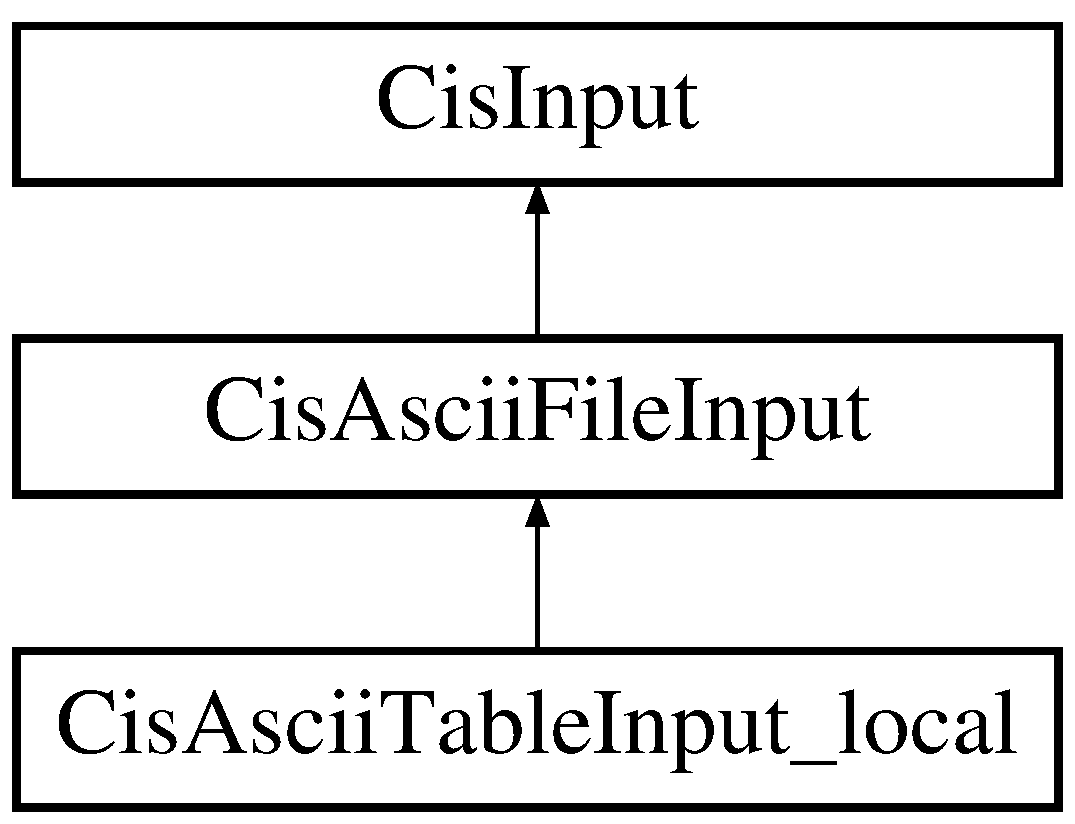
\includegraphics[height=3.000000cm]{classCisAsciiTableInput__local}
\end{center}
\end{figure}
\subsection*{Public Member Functions}
\begin{DoxyCompactItemize}
\item 
\mbox{\hyperlink{classCisAsciiTableInput__local_a1f7f46702f688c571b4c86617ef5035d}{Cis\+Ascii\+Table\+Input\+\_\+local}} (const char $\ast$name)
\begin{DoxyCompactList}\small\item\em Constructor for \mbox{\hyperlink{classCisAsciiTableInput__local}{Cis\+Ascii\+Table\+Input\+\_\+local}}. Due to issues with the C++ version of vsscanf, flags and precision indicators for floating point format specifiers (e.\+g. e, f), must be removed so that table input can be properly parsed. \end{DoxyCompactList}\end{DoxyCompactItemize}


\subsection{Detailed Description}
C++ interface to cis\+Ascii\+Table\+Input\+\_\+t functionality for local files. 

The \mbox{\hyperlink{classCisAsciiTableInput}{Cis\+Ascii\+Table\+Input}} class is a basic wrapper around the C cis\+Ascii\+Table\+Input\+\_\+t structure and associated functions from the \mbox{\hyperlink{CisInterface_8h_source}{Cis\+Interface.\+h}} header. It provides the user with C++ style access to basic A\+S\+C\+II table input operations. 

\subsection{Constructor \& Destructor Documentation}
\mbox{\Hypertarget{classCisAsciiTableInput__local_a1f7f46702f688c571b4c86617ef5035d}\label{classCisAsciiTableInput__local_a1f7f46702f688c571b4c86617ef5035d}} 
\index{Cis\+Ascii\+Table\+Input\+\_\+local@{Cis\+Ascii\+Table\+Input\+\_\+local}!Cis\+Ascii\+Table\+Input\+\_\+local@{Cis\+Ascii\+Table\+Input\+\_\+local}}
\index{Cis\+Ascii\+Table\+Input\+\_\+local@{Cis\+Ascii\+Table\+Input\+\_\+local}!Cis\+Ascii\+Table\+Input\+\_\+local@{Cis\+Ascii\+Table\+Input\+\_\+local}}
\subsubsection{\texorpdfstring{Cis\+Ascii\+Table\+Input\+\_\+local()}{CisAsciiTableInput\_local()}}
{\footnotesize\ttfamily Cis\+Ascii\+Table\+Input\+\_\+local\+::\+Cis\+Ascii\+Table\+Input\+\_\+local (\begin{DoxyParamCaption}\item[{const char $\ast$}]{name }\end{DoxyParamCaption})\hspace{0.3cm}{\ttfamily [inline]}}



Constructor for \mbox{\hyperlink{classCisAsciiTableInput__local}{Cis\+Ascii\+Table\+Input\+\_\+local}}. Due to issues with the C++ version of vsscanf, flags and precision indicators for floating point format specifiers (e.\+g. e, f), must be removed so that table input can be properly parsed. 


\begin{DoxyParams}[1]{Parameters}
\mbox{\tt in}  & {\em name} & constant character pointer to path of local table. \\
\hline
\end{DoxyParams}


The documentation for this class was generated from the following file\+:\begin{DoxyCompactItemize}
\item 
/root/cis\+\_\+interface/cis\+\_\+interface/cis\+\_\+interface/interface/Cis\+Interface.\+hpp\end{DoxyCompactItemize}

\hypertarget{classCisAsciiTableOutput}{}\section{Cis\+Ascii\+Table\+Output Class Reference}
\label{classCisAsciiTableOutput}\index{Cis\+Ascii\+Table\+Output@{Cis\+Ascii\+Table\+Output}}


C++ interface to cis\+Ascii\+Table\+Output\+\_\+t functionality.  




{\ttfamily \#include $<$Cis\+Interface.\+hpp$>$}

Inheritance diagram for Cis\+Ascii\+Table\+Output\+:\begin{figure}[H]
\begin{center}
\leavevmode
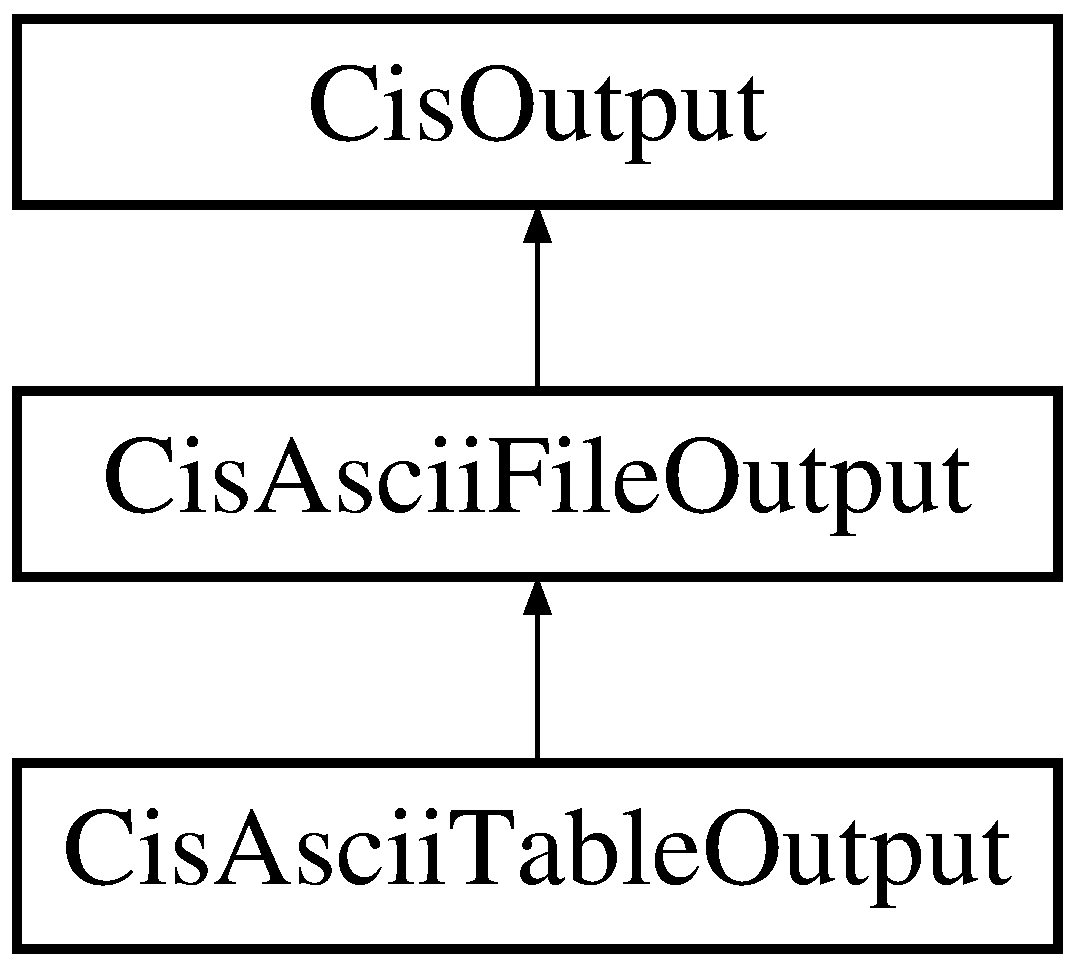
\includegraphics[height=3.000000cm]{classCisAsciiTableOutput}
\end{center}
\end{figure}
\subsection*{Public Member Functions}
\begin{DoxyCompactItemize}
\item 
\mbox{\hyperlink{classCisAsciiTableOutput_aa579418326a4192bf481e4e46fd3c170}{Cis\+Ascii\+Table\+Output}} (const char $\ast$name, const char $\ast$format\+\_\+str)
\begin{DoxyCompactList}\small\item\em Constructor for \mbox{\hyperlink{classCisAsciiTableOutput}{Cis\+Ascii\+Table\+Output}}. \end{DoxyCompactList}\end{DoxyCompactItemize}


\subsection{Detailed Description}
C++ interface to cis\+Ascii\+Table\+Output\+\_\+t functionality. 

The \mbox{\hyperlink{classCisAsciiTableOutput}{Cis\+Ascii\+Table\+Output}} class is a basic wrapper around the C cis\+Ascii\+Table\+Output\+\_\+t structure and associated functions from the \mbox{\hyperlink{CisInterface_8h_source}{Cis\+Interface.\+h}} header. It provides the user with C++ style access to basic A\+S\+C\+II table output operations. 

\subsection{Constructor \& Destructor Documentation}
\mbox{\Hypertarget{classCisAsciiTableOutput_aa579418326a4192bf481e4e46fd3c170}\label{classCisAsciiTableOutput_aa579418326a4192bf481e4e46fd3c170}} 
\index{Cis\+Ascii\+Table\+Output@{Cis\+Ascii\+Table\+Output}!Cis\+Ascii\+Table\+Output@{Cis\+Ascii\+Table\+Output}}
\index{Cis\+Ascii\+Table\+Output@{Cis\+Ascii\+Table\+Output}!Cis\+Ascii\+Table\+Output@{Cis\+Ascii\+Table\+Output}}
\subsubsection{\texorpdfstring{Cis\+Ascii\+Table\+Output()}{CisAsciiTableOutput()}}
{\footnotesize\ttfamily Cis\+Ascii\+Table\+Output\+::\+Cis\+Ascii\+Table\+Output (\begin{DoxyParamCaption}\item[{const char $\ast$}]{name,  }\item[{const char $\ast$}]{format\+\_\+str }\end{DoxyParamCaption})\hspace{0.3cm}{\ttfamily [inline]}}



Constructor for \mbox{\hyperlink{classCisAsciiTableOutput}{Cis\+Ascii\+Table\+Output}}. 


\begin{DoxyParams}[1]{Parameters}
\mbox{\tt in}  & {\em name} & constant character pointer to the name of an output channel. \\
\hline
\mbox{\tt in}  & {\em format\+\_\+str} & character pointer to format string that should be used to format rows into table lines. \\
\hline
\end{DoxyParams}


The documentation for this class was generated from the following file\+:\begin{DoxyCompactItemize}
\item 
/root/cis\+\_\+interface/cis\+\_\+interface/cis\+\_\+interface/interface/Cis\+Interface.\+hpp\end{DoxyCompactItemize}

\hypertarget{classCisAsciiTableOutput__local}{}\section{Cis\+Ascii\+Table\+Output\+\_\+local Class Reference}
\label{classCisAsciiTableOutput__local}\index{Cis\+Ascii\+Table\+Output\+\_\+local@{Cis\+Ascii\+Table\+Output\+\_\+local}}


C++ interface to cis\+Ascii\+Table\+Output\+\_\+t functionality for local files.  




{\ttfamily \#include $<$Cis\+Interface.\+hpp$>$}

Inheritance diagram for Cis\+Ascii\+Table\+Output\+\_\+local\+:\begin{figure}[H]
\begin{center}
\leavevmode
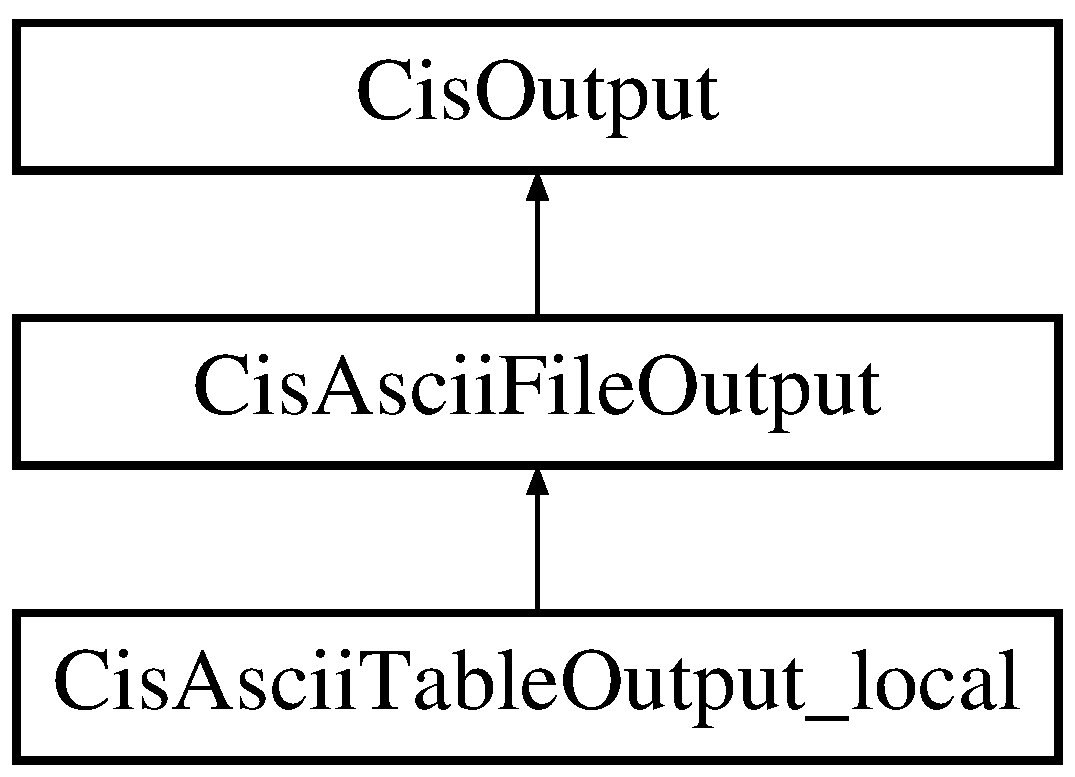
\includegraphics[height=3.000000cm]{classCisAsciiTableOutput__local}
\end{center}
\end{figure}
\subsection*{Public Member Functions}
\begin{DoxyCompactItemize}
\item 
\mbox{\hyperlink{classCisAsciiTableOutput__local_af18720ffabf013387aa1bcb8f8826ce3}{Cis\+Ascii\+Table\+Output\+\_\+local}} (const char $\ast$name, const char $\ast$format\+\_\+str)
\begin{DoxyCompactList}\small\item\em Constructor for \mbox{\hyperlink{classCisAsciiTableOutput}{Cis\+Ascii\+Table\+Output}} for local files. \end{DoxyCompactList}\end{DoxyCompactItemize}


\subsection{Detailed Description}
C++ interface to cis\+Ascii\+Table\+Output\+\_\+t functionality for local files. 

The \mbox{\hyperlink{classCisAsciiTableOutput}{Cis\+Ascii\+Table\+Output}} class is a basic wrapper around the C cis\+Ascii\+Table\+Output\+\_\+t structure and associated functions from the \mbox{\hyperlink{CisInterface_8h_source}{Cis\+Interface.\+h}} header. It provides the user with C++ style access to basic A\+S\+C\+II table output operations. 

\subsection{Constructor \& Destructor Documentation}
\mbox{\Hypertarget{classCisAsciiTableOutput__local_af18720ffabf013387aa1bcb8f8826ce3}\label{classCisAsciiTableOutput__local_af18720ffabf013387aa1bcb8f8826ce3}} 
\index{Cis\+Ascii\+Table\+Output\+\_\+local@{Cis\+Ascii\+Table\+Output\+\_\+local}!Cis\+Ascii\+Table\+Output\+\_\+local@{Cis\+Ascii\+Table\+Output\+\_\+local}}
\index{Cis\+Ascii\+Table\+Output\+\_\+local@{Cis\+Ascii\+Table\+Output\+\_\+local}!Cis\+Ascii\+Table\+Output\+\_\+local@{Cis\+Ascii\+Table\+Output\+\_\+local}}
\subsubsection{\texorpdfstring{Cis\+Ascii\+Table\+Output\+\_\+local()}{CisAsciiTableOutput\_local()}}
{\footnotesize\ttfamily Cis\+Ascii\+Table\+Output\+\_\+local\+::\+Cis\+Ascii\+Table\+Output\+\_\+local (\begin{DoxyParamCaption}\item[{const char $\ast$}]{name,  }\item[{const char $\ast$}]{format\+\_\+str }\end{DoxyParamCaption})\hspace{0.3cm}{\ttfamily [inline]}}



Constructor for \mbox{\hyperlink{classCisAsciiTableOutput}{Cis\+Ascii\+Table\+Output}} for local files. 


\begin{DoxyParams}[1]{Parameters}
\mbox{\tt in}  & {\em name} & constant character pointer to path of local table. \\
\hline
\mbox{\tt in}  & {\em format\+\_\+str} & character pointer to format string that should be used to format rows into table lines. \\
\hline
\end{DoxyParams}


The documentation for this class was generated from the following file\+:\begin{DoxyCompactItemize}
\item 
/root/cis\+\_\+interface/cis\+\_\+interface/cis\+\_\+interface/interface/Cis\+Interface.\+hpp\end{DoxyCompactItemize}

\hypertarget{classCisInput}{}\section{Cis\+Input Class Reference}
\label{classCisInput}\index{Cis\+Input@{Cis\+Input}}


Flag for checking if \mbox{\hyperlink{CisInterface_8hpp_source}{Cis\+Interface.\+hpp}} has already been included.  




{\ttfamily \#include $<$Cis\+Interface.\+hpp$>$}

Inheritance diagram for Cis\+Input\+:\begin{figure}[H]
\begin{center}
\leavevmode
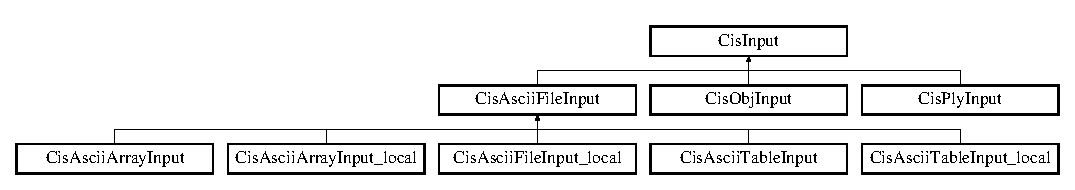
\includegraphics[height=2.100000cm]{classCisInput}
\end{center}
\end{figure}
\subsection*{Public Member Functions}
\begin{DoxyCompactItemize}
\item 
\mbox{\hyperlink{classCisInput_a5a81811ecb4ea9b3d786ea60522cdcb7}{Cis\+Input}} (const char $\ast$name)
\begin{DoxyCompactList}\small\item\em Constructor for \mbox{\hyperlink{classCisInput}{Cis\+Input}}. \end{DoxyCompactList}\item 
\mbox{\Hypertarget{classCisInput_a9e6a005bec40db9eacc4bd7c8051c112}\label{classCisInput_a9e6a005bec40db9eacc4bd7c8051c112}} 
\mbox{\hyperlink{classCisInput_a9e6a005bec40db9eacc4bd7c8051c112}{Cis\+Input}} (cis\+Input\+\_\+t x)
\begin{DoxyCompactList}\small\item\em Empty constructor for inheritance. \end{DoxyCompactList}\item 
\mbox{\hyperlink{classCisInput_ad39b94867de8741606bef7f1acdcbfd2}{Cis\+Input}} (const char $\ast$name, const char $\ast$fmt)
\begin{DoxyCompactList}\small\item\em Constructor for \mbox{\hyperlink{classCisInput}{Cis\+Input}} with format. \end{DoxyCompactList}\item 
\mbox{\Hypertarget{classCisInput_af098d058831c5aeb24c785daf322d0d3}\label{classCisInput_af098d058831c5aeb24c785daf322d0d3}} 
void \mbox{\hyperlink{classCisInput_af098d058831c5aeb24c785daf322d0d3}{\+\_\+destroy\+\_\+pi}} ()
\begin{DoxyCompactList}\small\item\em Alias to allow freeing of underlying C struct at the class level. \end{DoxyCompactList}\item 
\mbox{\Hypertarget{classCisInput_a66ff037c37e380abd82e107980f0af44}\label{classCisInput_a66ff037c37e380abd82e107980f0af44}} 
\mbox{\hyperlink{classCisInput_a66ff037c37e380abd82e107980f0af44}{$\sim$\+Cis\+Input}} ()
\begin{DoxyCompactList}\small\item\em Destructor for \mbox{\hyperlink{classCisInput}{Cis\+Input}}. See cis\+\_\+free in \mbox{\hyperlink{CisInterface_8h_source}{Cis\+Interface.\+h}} for details. \end{DoxyCompactList}\item 
cis\+Input\+\_\+t \mbox{\hyperlink{classCisInput_a2b560759fbd797db1dc049e886ce72e5}{pi}} ()
\begin{DoxyCompactList}\small\item\em Return the cis\+Input\+\_\+t structure. \end{DoxyCompactList}\item 
int \mbox{\hyperlink{classCisInput_aa05f26dd9d8db09e12da739831637a2a}{recv}} (char $\ast$data, const size\+\_\+t len)
\begin{DoxyCompactList}\small\item\em Receive a message shorter than C\+I\+S\+\_\+\+M\+S\+G\+\_\+\+M\+AX from the input queue. See cis\+\_\+recv in \mbox{\hyperlink{CisInterface_8h_source}{Cis\+Interface.\+h}} for additional details. \end{DoxyCompactList}\item 
int \mbox{\hyperlink{classCisInput_a387134ab4f750a06654946d4b92d412d}{recv}} (const int nargs,...)
\begin{DoxyCompactList}\small\item\em Receive and parse a message shorter than C\+I\+S\+\_\+\+M\+S\+G\+\_\+\+M\+AX from the input queue. See cis\+Recv from \mbox{\hyperlink{CisInterface_8h_source}{Cis\+Interface.\+h}} for details. \end{DoxyCompactList}\item 
int \mbox{\hyperlink{classCisInput_a962f5ebcac9d8b70fe3cd907da6dd3a9}{recv\+\_\+nolimit}} (char $\ast$$\ast$data, const size\+\_\+t len)
\begin{DoxyCompactList}\small\item\em Receive a message larger than C\+I\+S\+\_\+\+M\+S\+G\+\_\+\+M\+AX from the input queue. See cis\+\_\+recv\+\_\+nolimit in \mbox{\hyperlink{CisInterface_8h_source}{Cis\+Interface.\+h}} for additional details. \end{DoxyCompactList}\item 
int \mbox{\hyperlink{classCisInput_aa78610915e128dc1ed0d234271d2d656}{recv\+\_\+nolimit}} (const int nargs,...)
\begin{DoxyCompactList}\small\item\em Receive and parse a message larger than C\+I\+S\+\_\+\+M\+S\+G\+\_\+\+M\+AX from the input queue. See cis\+Recv\+\_\+nolimit from \mbox{\hyperlink{CisInterface_8h_source}{Cis\+Interface.\+h}} for details. \end{DoxyCompactList}\end{DoxyCompactItemize}


\subsection{Detailed Description}
Flag for checking if \mbox{\hyperlink{CisInterface_8hpp_source}{Cis\+Interface.\+hpp}} has already been included. 

C++ interface to cis\+Input\+\_\+t functionality.

The \mbox{\hyperlink{classCisInput}{Cis\+Input}} class is a basic wrapper around the C cis\+Input\+\_\+t structure and associated functions from the \mbox{\hyperlink{CisInterface_8h_source}{Cis\+Interface.\+h}} header. It provides the user with C++ style access to basic input via an I\+PC queue. 

\subsection{Constructor \& Destructor Documentation}
\mbox{\Hypertarget{classCisInput_a5a81811ecb4ea9b3d786ea60522cdcb7}\label{classCisInput_a5a81811ecb4ea9b3d786ea60522cdcb7}} 
\index{Cis\+Input@{Cis\+Input}!Cis\+Input@{Cis\+Input}}
\index{Cis\+Input@{Cis\+Input}!Cis\+Input@{Cis\+Input}}
\subsubsection{\texorpdfstring{Cis\+Input()}{CisInput()}\hspace{0.1cm}{\footnotesize\ttfamily [1/2]}}
{\footnotesize\ttfamily Cis\+Input\+::\+Cis\+Input (\begin{DoxyParamCaption}\item[{const char $\ast$}]{name }\end{DoxyParamCaption})\hspace{0.3cm}{\ttfamily [inline]}}



Constructor for \mbox{\hyperlink{classCisInput}{Cis\+Input}}. 


\begin{DoxyParams}[1]{Parameters}
\mbox{\tt in}  & {\em name} & constant character pointer to name of input queue. This should be the argument to an input driver in the yaml specification file. \\
\hline
\end{DoxyParams}
\mbox{\Hypertarget{classCisInput_ad39b94867de8741606bef7f1acdcbfd2}\label{classCisInput_ad39b94867de8741606bef7f1acdcbfd2}} 
\index{Cis\+Input@{Cis\+Input}!Cis\+Input@{Cis\+Input}}
\index{Cis\+Input@{Cis\+Input}!Cis\+Input@{Cis\+Input}}
\subsubsection{\texorpdfstring{Cis\+Input()}{CisInput()}\hspace{0.1cm}{\footnotesize\ttfamily [2/2]}}
{\footnotesize\ttfamily Cis\+Input\+::\+Cis\+Input (\begin{DoxyParamCaption}\item[{const char $\ast$}]{name,  }\item[{const char $\ast$}]{fmt }\end{DoxyParamCaption})\hspace{0.3cm}{\ttfamily [inline]}}



Constructor for \mbox{\hyperlink{classCisInput}{Cis\+Input}} with format. 


\begin{DoxyParams}[1]{Parameters}
\mbox{\tt in}  & {\em name} & constant character pointer to name of input queue. This should be the argument to an input driver in the yaml specification file. \\
\hline
\mbox{\tt in}  & {\em fmt} & character pointer to format string for parsing messages. \\
\hline
\end{DoxyParams}


\subsection{Member Function Documentation}
\mbox{\Hypertarget{classCisInput_a2b560759fbd797db1dc049e886ce72e5}\label{classCisInput_a2b560759fbd797db1dc049e886ce72e5}} 
\index{Cis\+Input@{Cis\+Input}!pi@{pi}}
\index{pi@{pi}!Cis\+Input@{Cis\+Input}}
\subsubsection{\texorpdfstring{pi()}{pi()}}
{\footnotesize\ttfamily cis\+Input\+\_\+t Cis\+Input\+::pi (\begin{DoxyParamCaption}{ }\end{DoxyParamCaption})\hspace{0.3cm}{\ttfamily [inline]}}



Return the cis\+Input\+\_\+t structure. 

\begin{DoxyReturn}{Returns}
cis\+Input\+\_\+t structure underlying the class. 
\end{DoxyReturn}
\mbox{\Hypertarget{classCisInput_aa05f26dd9d8db09e12da739831637a2a}\label{classCisInput_aa05f26dd9d8db09e12da739831637a2a}} 
\index{Cis\+Input@{Cis\+Input}!recv@{recv}}
\index{recv@{recv}!Cis\+Input@{Cis\+Input}}
\subsubsection{\texorpdfstring{recv()}{recv()}\hspace{0.1cm}{\footnotesize\ttfamily [1/2]}}
{\footnotesize\ttfamily int Cis\+Input\+::recv (\begin{DoxyParamCaption}\item[{char $\ast$}]{data,  }\item[{const size\+\_\+t}]{len }\end{DoxyParamCaption})\hspace{0.3cm}{\ttfamily [inline]}}



Receive a message shorter than C\+I\+S\+\_\+\+M\+S\+G\+\_\+\+M\+AX from the input queue. See cis\+\_\+recv in \mbox{\hyperlink{CisInterface_8h_source}{Cis\+Interface.\+h}} for additional details. 


\begin{DoxyParams}[1]{Parameters}
\mbox{\tt out}  & {\em data} & character pointer to allocated buffer where the message should be saved. \\
\hline
\mbox{\tt in}  & {\em len} & size\+\_\+t length of the allocated message buffer in bytes. \\
\hline
\end{DoxyParams}
\begin{DoxyReturn}{Returns}
int -\/1 if message could not be received. Length of the received message if message was received. 
\end{DoxyReturn}
\mbox{\Hypertarget{classCisInput_a387134ab4f750a06654946d4b92d412d}\label{classCisInput_a387134ab4f750a06654946d4b92d412d}} 
\index{Cis\+Input@{Cis\+Input}!recv@{recv}}
\index{recv@{recv}!Cis\+Input@{Cis\+Input}}
\subsubsection{\texorpdfstring{recv()}{recv()}\hspace{0.1cm}{\footnotesize\ttfamily [2/2]}}
{\footnotesize\ttfamily int Cis\+Input\+::recv (\begin{DoxyParamCaption}\item[{const int}]{nargs,  }\item[{}]{... }\end{DoxyParamCaption})\hspace{0.3cm}{\ttfamily [inline]}}



Receive and parse a message shorter than C\+I\+S\+\_\+\+M\+S\+G\+\_\+\+M\+AX from the input queue. See cis\+Recv from \mbox{\hyperlink{CisInterface_8h_source}{Cis\+Interface.\+h}} for details. 


\begin{DoxyParams}[1]{Parameters}
\mbox{\tt in}  & {\em nargs} & int Number of arguments being passed. \\
\hline
\mbox{\tt out}  & {\em ...} & mixed arguments that should be assigned parameters extracted using the format string. Since these will be assigned, they should be pointers to memory that has already been allocated. \\
\hline
\end{DoxyParams}
\begin{DoxyReturn}{Returns}
integer specifying if the receive was succesful. Values $>$= 0 indicate success. 
\end{DoxyReturn}
\mbox{\Hypertarget{classCisInput_a962f5ebcac9d8b70fe3cd907da6dd3a9}\label{classCisInput_a962f5ebcac9d8b70fe3cd907da6dd3a9}} 
\index{Cis\+Input@{Cis\+Input}!recv\+\_\+nolimit@{recv\+\_\+nolimit}}
\index{recv\+\_\+nolimit@{recv\+\_\+nolimit}!Cis\+Input@{Cis\+Input}}
\subsubsection{\texorpdfstring{recv\+\_\+nolimit()}{recv\_nolimit()}\hspace{0.1cm}{\footnotesize\ttfamily [1/2]}}
{\footnotesize\ttfamily int Cis\+Input\+::recv\+\_\+nolimit (\begin{DoxyParamCaption}\item[{char $\ast$$\ast$}]{data,  }\item[{const size\+\_\+t}]{len }\end{DoxyParamCaption})\hspace{0.3cm}{\ttfamily [inline]}}



Receive a message larger than C\+I\+S\+\_\+\+M\+S\+G\+\_\+\+M\+AX from the input queue. See cis\+\_\+recv\+\_\+nolimit in \mbox{\hyperlink{CisInterface_8h_source}{Cis\+Interface.\+h}} for additional details. 


\begin{DoxyParams}[1]{Parameters}
\mbox{\tt out}  & {\em data} & character pointer to allocated buffer where the message should be saved. \\
\hline
\mbox{\tt in}  & {\em len} & size\+\_\+t length of the allocated message buffer in bytes. \\
\hline
\end{DoxyParams}
\begin{DoxyReturn}{Returns}
int -\/1 if message could not be received. Length of the received message if message was received. 
\end{DoxyReturn}
\mbox{\Hypertarget{classCisInput_aa78610915e128dc1ed0d234271d2d656}\label{classCisInput_aa78610915e128dc1ed0d234271d2d656}} 
\index{Cis\+Input@{Cis\+Input}!recv\+\_\+nolimit@{recv\+\_\+nolimit}}
\index{recv\+\_\+nolimit@{recv\+\_\+nolimit}!Cis\+Input@{Cis\+Input}}
\subsubsection{\texorpdfstring{recv\+\_\+nolimit()}{recv\_nolimit()}\hspace{0.1cm}{\footnotesize\ttfamily [2/2]}}
{\footnotesize\ttfamily int Cis\+Input\+::recv\+\_\+nolimit (\begin{DoxyParamCaption}\item[{const int}]{nargs,  }\item[{}]{... }\end{DoxyParamCaption})\hspace{0.3cm}{\ttfamily [inline]}}



Receive and parse a message larger than C\+I\+S\+\_\+\+M\+S\+G\+\_\+\+M\+AX from the input queue. See cis\+Recv\+\_\+nolimit from \mbox{\hyperlink{CisInterface_8h_source}{Cis\+Interface.\+h}} for details. 


\begin{DoxyParams}[1]{Parameters}
\mbox{\tt in}  & {\em nargs} & int Number of arguments being passed. \\
\hline
\mbox{\tt out}  & {\em ...} & mixed arguments that should be assigned parameters extracted using the format string. Since these will be assigned, they should be pointers to memory that has already been allocated. \\
\hline
\end{DoxyParams}
\begin{DoxyReturn}{Returns}
integer specifying if the receive was succesful. Values $>$= 0 indicate success. 
\end{DoxyReturn}


The documentation for this class was generated from the following file\+:\begin{DoxyCompactItemize}
\item 
/root/cis\+\_\+interface/cis\+\_\+interface/cis\+\_\+interface/interface/Cis\+Interface.\+hpp\end{DoxyCompactItemize}

\hypertarget{classCisObjInput}{}\section{Cis\+Obj\+Input Class Reference}
\label{classCisObjInput}\index{Cis\+Obj\+Input@{Cis\+Obj\+Input}}


C++ interface to cis\+Obj\+Input\+\_\+t functionality. The \mbox{\hyperlink{classCisObjInput}{Cis\+Obj\+Input}} class is a basic wrapper around the C cis\+Obj\+Input\+\_\+t structure and associated functions from the \mbox{\hyperlink{CisInterface_8h_source}{Cis\+Interface.\+h}} header. It provides the user with C++ style access to basic A\+S\+C\+II file input operations.  




{\ttfamily \#include $<$Cis\+Interface.\+hpp$>$}

Inheritance diagram for Cis\+Obj\+Input\+:\begin{figure}[H]
\begin{center}
\leavevmode
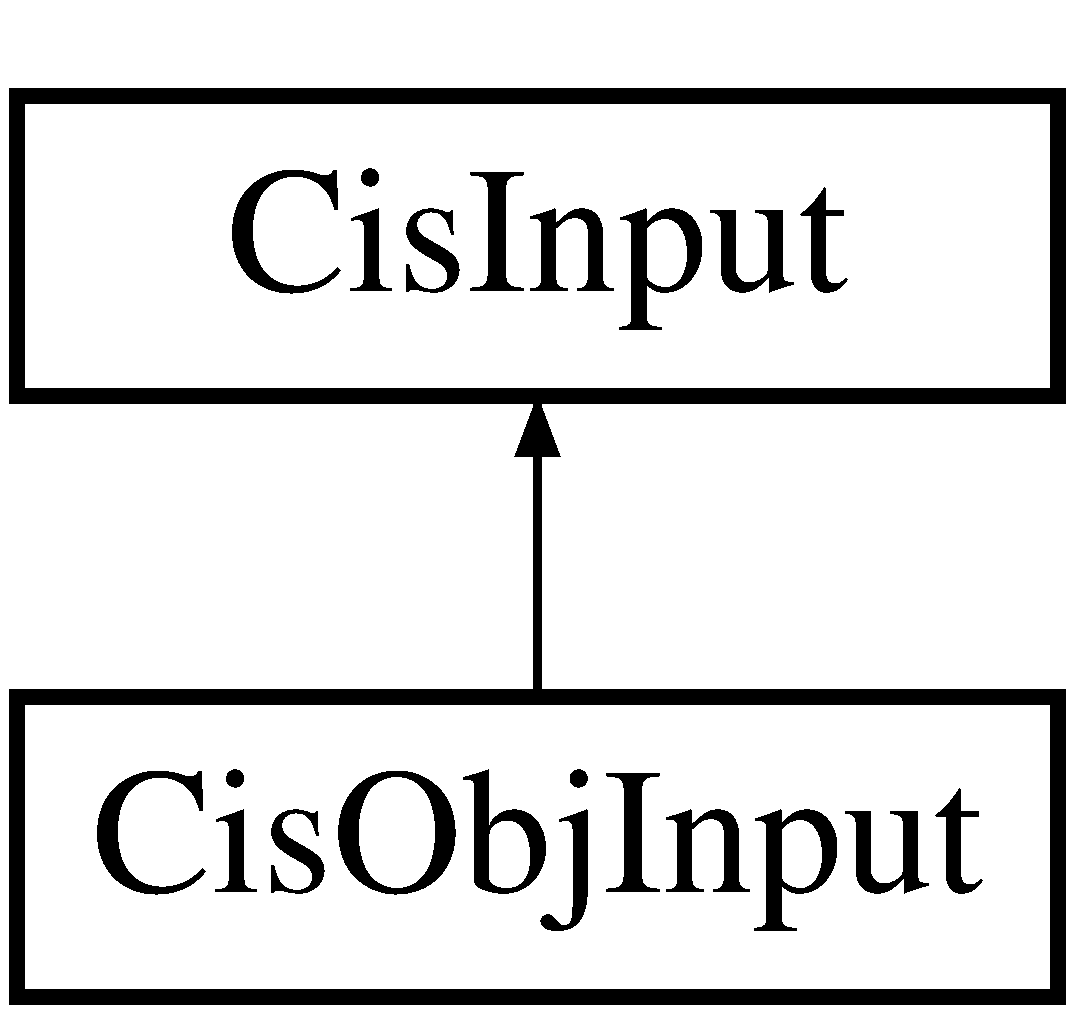
\includegraphics[height=2.000000cm]{classCisObjInput}
\end{center}
\end{figure}
\subsection*{Public Member Functions}
\begin{DoxyCompactItemize}
\item 
\mbox{\hyperlink{classCisObjInput_a76dfa86d8de7415db586f5993271c5fe}{Cis\+Obj\+Input}} (const char $\ast$name)
\begin{DoxyCompactList}\small\item\em Constructor for \mbox{\hyperlink{classCisObjInput}{Cis\+Obj\+Input}}. \end{DoxyCompactList}\item 
\mbox{\Hypertarget{classCisObjInput_a159e6c8945d6fa7fd8361a045255eddb}\label{classCisObjInput_a159e6c8945d6fa7fd8361a045255eddb}} 
\mbox{\hyperlink{classCisObjInput_a159e6c8945d6fa7fd8361a045255eddb}{Cis\+Obj\+Input}} (cis\+Input\+\_\+t x)
\begin{DoxyCompactList}\small\item\em Empty constructor for inheritance. \end{DoxyCompactList}\end{DoxyCompactItemize}


\subsection{Detailed Description}
C++ interface to cis\+Obj\+Input\+\_\+t functionality. The \mbox{\hyperlink{classCisObjInput}{Cis\+Obj\+Input}} class is a basic wrapper around the C cis\+Obj\+Input\+\_\+t structure and associated functions from the \mbox{\hyperlink{CisInterface_8h_source}{Cis\+Interface.\+h}} header. It provides the user with C++ style access to basic A\+S\+C\+II file input operations. 

\subsection{Constructor \& Destructor Documentation}
\mbox{\Hypertarget{classCisObjInput_a76dfa86d8de7415db586f5993271c5fe}\label{classCisObjInput_a76dfa86d8de7415db586f5993271c5fe}} 
\index{Cis\+Obj\+Input@{Cis\+Obj\+Input}!Cis\+Obj\+Input@{Cis\+Obj\+Input}}
\index{Cis\+Obj\+Input@{Cis\+Obj\+Input}!Cis\+Obj\+Input@{Cis\+Obj\+Input}}
\subsubsection{\texorpdfstring{Cis\+Obj\+Input()}{CisObjInput()}}
{\footnotesize\ttfamily Cis\+Obj\+Input\+::\+Cis\+Obj\+Input (\begin{DoxyParamCaption}\item[{const char $\ast$}]{name }\end{DoxyParamCaption})\hspace{0.3cm}{\ttfamily [inline]}}



Constructor for \mbox{\hyperlink{classCisObjInput}{Cis\+Obj\+Input}}. 


\begin{DoxyParams}[1]{Parameters}
\mbox{\tt in}  & {\em name} & constant character pointer to the name of an input channel. \\
\hline
\end{DoxyParams}


The documentation for this class was generated from the following file\+:\begin{DoxyCompactItemize}
\item 
/root/cis\+\_\+interface/cis\+\_\+interface/cis\+\_\+interface/interface/Cis\+Interface.\+hpp\end{DoxyCompactItemize}

\hypertarget{classCisObjOutput}{}\section{Cis\+Obj\+Output Class Reference}
\label{classCisObjOutput}\index{Cis\+Obj\+Output@{Cis\+Obj\+Output}}


C++ interface to cis\+Obj\+Output\+\_\+t functionality. The \mbox{\hyperlink{classCisObjOutput}{Cis\+Obj\+Output}} class is a basic wrapper around the C cis\+Obj\+Output\+\_\+t structure and associated functions from the \mbox{\hyperlink{CisInterface_8h_source}{Cis\+Interface.\+h}} header. It provides the user with C++ style access to basic A\+S\+C\+II file output operations.  




{\ttfamily \#include $<$Cis\+Interface.\+hpp$>$}

Inheritance diagram for Cis\+Obj\+Output\+:\begin{figure}[H]
\begin{center}
\leavevmode
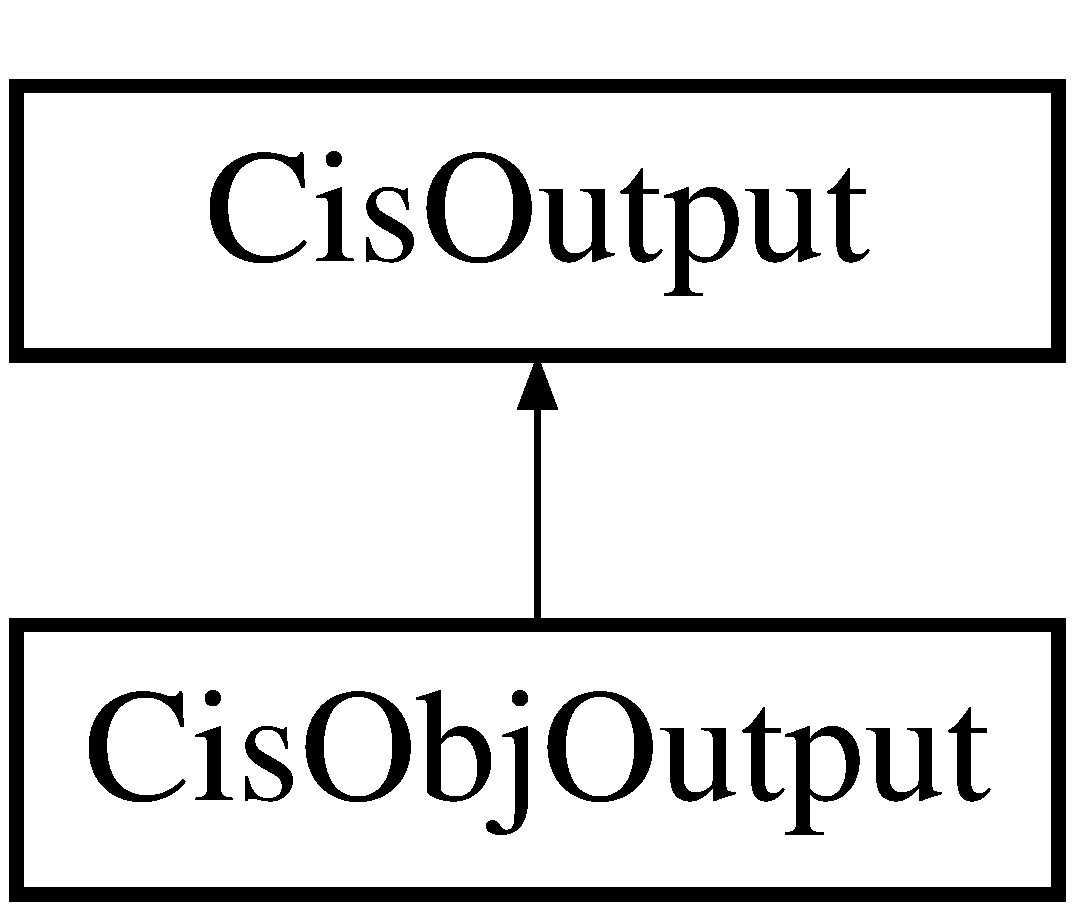
\includegraphics[height=2.000000cm]{classCisObjOutput}
\end{center}
\end{figure}
\subsection*{Public Member Functions}
\begin{DoxyCompactItemize}
\item 
\mbox{\hyperlink{classCisObjOutput_afb7eecc9487342188c292e4a6889fee9}{Cis\+Obj\+Output}} (const char $\ast$name)
\begin{DoxyCompactList}\small\item\em Constructor for \mbox{\hyperlink{classCisObjOutput}{Cis\+Obj\+Output}}. \end{DoxyCompactList}\item 
\mbox{\Hypertarget{classCisObjOutput_a0788a59b74f38c7bfd27b21fd39386e7}\label{classCisObjOutput_a0788a59b74f38c7bfd27b21fd39386e7}} 
\mbox{\hyperlink{classCisObjOutput_a0788a59b74f38c7bfd27b21fd39386e7}{Cis\+Obj\+Output}} (cis\+Output\+\_\+t x)
\begin{DoxyCompactList}\small\item\em Empty constructor for inheritance. \end{DoxyCompactList}\end{DoxyCompactItemize}


\subsection{Detailed Description}
C++ interface to cis\+Obj\+Output\+\_\+t functionality. The \mbox{\hyperlink{classCisObjOutput}{Cis\+Obj\+Output}} class is a basic wrapper around the C cis\+Obj\+Output\+\_\+t structure and associated functions from the \mbox{\hyperlink{CisInterface_8h_source}{Cis\+Interface.\+h}} header. It provides the user with C++ style access to basic A\+S\+C\+II file output operations. 

\subsection{Constructor \& Destructor Documentation}
\mbox{\Hypertarget{classCisObjOutput_afb7eecc9487342188c292e4a6889fee9}\label{classCisObjOutput_afb7eecc9487342188c292e4a6889fee9}} 
\index{Cis\+Obj\+Output@{Cis\+Obj\+Output}!Cis\+Obj\+Output@{Cis\+Obj\+Output}}
\index{Cis\+Obj\+Output@{Cis\+Obj\+Output}!Cis\+Obj\+Output@{Cis\+Obj\+Output}}
\subsubsection{\texorpdfstring{Cis\+Obj\+Output()}{CisObjOutput()}}
{\footnotesize\ttfamily Cis\+Obj\+Output\+::\+Cis\+Obj\+Output (\begin{DoxyParamCaption}\item[{const char $\ast$}]{name }\end{DoxyParamCaption})\hspace{0.3cm}{\ttfamily [inline]}}



Constructor for \mbox{\hyperlink{classCisObjOutput}{Cis\+Obj\+Output}}. 


\begin{DoxyParams}[1]{Parameters}
\mbox{\tt in}  & {\em name} & constant character pointer to the name of an output channel. \\
\hline
\end{DoxyParams}


The documentation for this class was generated from the following file\+:\begin{DoxyCompactItemize}
\item 
/root/cis\+\_\+interface/cis\+\_\+interface/cis\+\_\+interface/interface/Cis\+Interface.\+hpp\end{DoxyCompactItemize}

\hypertarget{classCisOutput}{}\section{Cis\+Output Class Reference}
\label{classCisOutput}\index{Cis\+Output@{Cis\+Output}}


C++ interface to cis\+Output\+\_\+t functionality.  




{\ttfamily \#include $<$Cis\+Interface.\+hpp$>$}

Inheritance diagram for Cis\+Output\+:\begin{figure}[H]
\begin{center}
\leavevmode
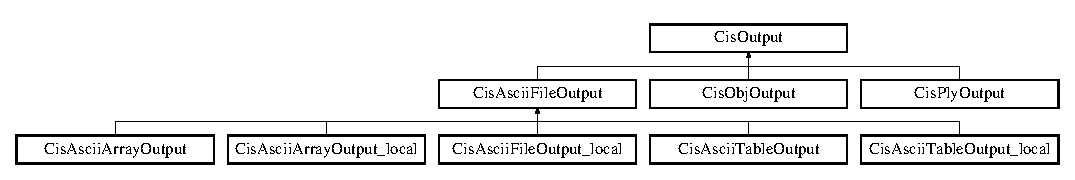
\includegraphics[height=1.976471cm]{classCisOutput}
\end{center}
\end{figure}
\subsection*{Public Member Functions}
\begin{DoxyCompactItemize}
\item 
\mbox{\hyperlink{classCisOutput_acbe5281010e3dd4617006a03d9c6c06c}{Cis\+Output}} (const char $\ast$name)
\begin{DoxyCompactList}\small\item\em Constructor for \mbox{\hyperlink{classCisOutput}{Cis\+Output}}. \end{DoxyCompactList}\item 
\mbox{\hyperlink{classCisOutput_a276eaee68d97cba54726752784d6c4df}{Cis\+Output}} (const char $\ast$name, const char $\ast$fmt)
\begin{DoxyCompactList}\small\item\em Constructor for \mbox{\hyperlink{classCisOutput}{Cis\+Output}} with format. \end{DoxyCompactList}\item 
\mbox{\Hypertarget{classCisOutput_abf373bf8e55beb4b32d558463b134a51}\label{classCisOutput_abf373bf8e55beb4b32d558463b134a51}} 
\mbox{\hyperlink{classCisOutput_abf373bf8e55beb4b32d558463b134a51}{Cis\+Output}} (cis\+Output\+\_\+t x)
\begin{DoxyCompactList}\small\item\em Empty constructor for inheritance. \end{DoxyCompactList}\item 
\mbox{\Hypertarget{classCisOutput_af977def262b778702e06277f5d50f102}\label{classCisOutput_af977def262b778702e06277f5d50f102}} 
void \mbox{\hyperlink{classCisOutput_af977def262b778702e06277f5d50f102}{\+\_\+destroy\+\_\+pi}} ()
\begin{DoxyCompactList}\small\item\em Alias to allow freeing of underlying C struct at the class level. \end{DoxyCompactList}\item 
\mbox{\Hypertarget{classCisOutput_a7dc7c92d8c50f61075d1ef0cf0dfce8f}\label{classCisOutput_a7dc7c92d8c50f61075d1ef0cf0dfce8f}} 
\mbox{\hyperlink{classCisOutput_a7dc7c92d8c50f61075d1ef0cf0dfce8f}{$\sim$\+Cis\+Output}} ()
\begin{DoxyCompactList}\small\item\em Destructor for \mbox{\hyperlink{classCisOutput}{Cis\+Output}}. See cis\+\_\+free in \mbox{\hyperlink{CisInterface_8h_source}{Cis\+Interface.\+h}} for details. \end{DoxyCompactList}\item 
cis\+Output\+\_\+t \mbox{\hyperlink{classCisOutput_a173ffd20bb1ce255ba95562caa220d6a}{pi}} ()
\begin{DoxyCompactList}\small\item\em Return the cis\+Output\+\_\+t structure. \end{DoxyCompactList}\item 
int \mbox{\hyperlink{classCisOutput_a38322e95e9743e4b5b5d4c529d13031e}{send}} (const char $\ast$data, const size\+\_\+t len)
\begin{DoxyCompactList}\small\item\em Send a message smaller than C\+I\+S\+\_\+\+M\+S\+G\+\_\+\+M\+AX to the output queue. If the message is larger than C\+I\+S\+\_\+\+M\+S\+G\+\_\+\+M\+AX an error code will be returned. See cis\+\_\+send in \mbox{\hyperlink{CisInterface_8h_source}{Cis\+Interface.\+h}} for details. \end{DoxyCompactList}\item 
int \mbox{\hyperlink{classCisOutput_ad30d4a8e64e7a9b7033cddf4a3aef9de}{send}} (const int nargs,...)
\begin{DoxyCompactList}\small\item\em Format and send a message smaller than C\+I\+S\+\_\+\+M\+S\+G\+\_\+\+M\+AX to the output queue. See cis\+Send from \mbox{\hyperlink{CisInterface_8h_source}{Cis\+Interface.\+h}} for details. \end{DoxyCompactList}\item 
int \mbox{\hyperlink{classCisOutput_a794b0e4d24de72339faab690554db4d3}{send\+\_\+nolimit}} (const char $\ast$data, const size\+\_\+t len)
\begin{DoxyCompactList}\small\item\em Send a message larger than C\+I\+S\+\_\+\+M\+S\+G\+\_\+\+M\+AX to the output queue. See cis\+\_\+send\+\_\+nolimit in \mbox{\hyperlink{CisInterface_8h_source}{Cis\+Interface.\+h}} for details. \end{DoxyCompactList}\item 
int \mbox{\hyperlink{classCisOutput_a5b7e84b70352f3a5f99650184a076564}{send\+\_\+nolimit}} (const int nargs,...)
\begin{DoxyCompactList}\small\item\em Format and send a message larger than C\+I\+S\+\_\+\+M\+S\+G\+\_\+\+M\+AX to the output queue. See cis\+Send from \mbox{\hyperlink{CisInterface_8h_source}{Cis\+Interface.\+h}} for details. \end{DoxyCompactList}\item 
int \mbox{\hyperlink{classCisOutput_a083fb17afbb3c03f103929850506e545}{send\+\_\+eof}} ()
\begin{DoxyCompactList}\small\item\em Send E\+OF message to output file, closing it. \end{DoxyCompactList}\end{DoxyCompactItemize}


\subsection{Detailed Description}
C++ interface to cis\+Output\+\_\+t functionality. 

The \mbox{\hyperlink{classCisOutput}{Cis\+Output}} class is a basic wrapper around the C cis\+Output\+\_\+t structure and associated functions from the \mbox{\hyperlink{CisInterface_8h_source}{Cis\+Interface.\+h}} header. It provides the user with C++ style access to basic output via an I\+PC queue. 

\subsection{Constructor \& Destructor Documentation}
\mbox{\Hypertarget{classCisOutput_acbe5281010e3dd4617006a03d9c6c06c}\label{classCisOutput_acbe5281010e3dd4617006a03d9c6c06c}} 
\index{Cis\+Output@{Cis\+Output}!Cis\+Output@{Cis\+Output}}
\index{Cis\+Output@{Cis\+Output}!Cis\+Output@{Cis\+Output}}
\subsubsection{\texorpdfstring{Cis\+Output()}{CisOutput()}\hspace{0.1cm}{\footnotesize\ttfamily [1/2]}}
{\footnotesize\ttfamily Cis\+Output\+::\+Cis\+Output (\begin{DoxyParamCaption}\item[{const char $\ast$}]{name }\end{DoxyParamCaption})\hspace{0.3cm}{\ttfamily [inline]}}



Constructor for \mbox{\hyperlink{classCisOutput}{Cis\+Output}}. 


\begin{DoxyParams}[1]{Parameters}
\mbox{\tt in}  & {\em name} & constant character pointer to name of output queue. This should be the argument to an output driver in the yaml specification file. \\
\hline
\end{DoxyParams}
\mbox{\Hypertarget{classCisOutput_a276eaee68d97cba54726752784d6c4df}\label{classCisOutput_a276eaee68d97cba54726752784d6c4df}} 
\index{Cis\+Output@{Cis\+Output}!Cis\+Output@{Cis\+Output}}
\index{Cis\+Output@{Cis\+Output}!Cis\+Output@{Cis\+Output}}
\subsubsection{\texorpdfstring{Cis\+Output()}{CisOutput()}\hspace{0.1cm}{\footnotesize\ttfamily [2/2]}}
{\footnotesize\ttfamily Cis\+Output\+::\+Cis\+Output (\begin{DoxyParamCaption}\item[{const char $\ast$}]{name,  }\item[{const char $\ast$}]{fmt }\end{DoxyParamCaption})\hspace{0.3cm}{\ttfamily [inline]}}



Constructor for \mbox{\hyperlink{classCisOutput}{Cis\+Output}} with format. 


\begin{DoxyParams}[1]{Parameters}
\mbox{\tt in}  & {\em name} & constant character pointer to name of output queue. This should be the argument to an output driver in the yaml specification file. \\
\hline
\mbox{\tt in}  & {\em fmt} & character pointer to format string for formatting variables. \\
\hline
\end{DoxyParams}


\subsection{Member Function Documentation}
\mbox{\Hypertarget{classCisOutput_a173ffd20bb1ce255ba95562caa220d6a}\label{classCisOutput_a173ffd20bb1ce255ba95562caa220d6a}} 
\index{Cis\+Output@{Cis\+Output}!pi@{pi}}
\index{pi@{pi}!Cis\+Output@{Cis\+Output}}
\subsubsection{\texorpdfstring{pi()}{pi()}}
{\footnotesize\ttfamily cis\+Output\+\_\+t Cis\+Output\+::pi (\begin{DoxyParamCaption}{ }\end{DoxyParamCaption})\hspace{0.3cm}{\ttfamily [inline]}}



Return the cis\+Output\+\_\+t structure. 

\begin{DoxyReturn}{Returns}
cis\+Output\+\_\+t structure underlying the class. 
\end{DoxyReturn}
\mbox{\Hypertarget{classCisOutput_a38322e95e9743e4b5b5d4c529d13031e}\label{classCisOutput_a38322e95e9743e4b5b5d4c529d13031e}} 
\index{Cis\+Output@{Cis\+Output}!send@{send}}
\index{send@{send}!Cis\+Output@{Cis\+Output}}
\subsubsection{\texorpdfstring{send()}{send()}\hspace{0.1cm}{\footnotesize\ttfamily [1/2]}}
{\footnotesize\ttfamily int Cis\+Output\+::send (\begin{DoxyParamCaption}\item[{const char $\ast$}]{data,  }\item[{const size\+\_\+t}]{len }\end{DoxyParamCaption})\hspace{0.3cm}{\ttfamily [inline]}}



Send a message smaller than C\+I\+S\+\_\+\+M\+S\+G\+\_\+\+M\+AX to the output queue. If the message is larger than C\+I\+S\+\_\+\+M\+S\+G\+\_\+\+M\+AX an error code will be returned. See cis\+\_\+send in \mbox{\hyperlink{CisInterface_8h_source}{Cis\+Interface.\+h}} for details. 


\begin{DoxyParams}[1]{Parameters}
\mbox{\tt in}  & {\em data} & character pointer to message that should be sent. \\
\hline
\mbox{\tt in}  & {\em len} & size\+\_\+t length of message to be sent. \\
\hline
\end{DoxyParams}
\begin{DoxyReturn}{Returns}
int 0 if send succesfull, -\/1 if send unsuccessful. 
\end{DoxyReturn}
\mbox{\Hypertarget{classCisOutput_ad30d4a8e64e7a9b7033cddf4a3aef9de}\label{classCisOutput_ad30d4a8e64e7a9b7033cddf4a3aef9de}} 
\index{Cis\+Output@{Cis\+Output}!send@{send}}
\index{send@{send}!Cis\+Output@{Cis\+Output}}
\subsubsection{\texorpdfstring{send()}{send()}\hspace{0.1cm}{\footnotesize\ttfamily [2/2]}}
{\footnotesize\ttfamily int Cis\+Output\+::send (\begin{DoxyParamCaption}\item[{const int}]{nargs,  }\item[{}]{... }\end{DoxyParamCaption})\hspace{0.3cm}{\ttfamily [inline]}}



Format and send a message smaller than C\+I\+S\+\_\+\+M\+S\+G\+\_\+\+M\+AX to the output queue. See cis\+Send from \mbox{\hyperlink{CisInterface_8h_source}{Cis\+Interface.\+h}} for details. 


\begin{DoxyParams}[1]{Parameters}
\mbox{\tt in}  & {\em nargs} & int Number of arguments being passed. \\
\hline
\mbox{\tt in}  & {\em ...} & arguments for formatting. ~\newline
\\
\hline
\end{DoxyParams}
\begin{DoxyReturn}{Returns}
integer specifying if the send was succesful. Values $>$= 0 indicate success. 
\end{DoxyReturn}
\mbox{\Hypertarget{classCisOutput_a083fb17afbb3c03f103929850506e545}\label{classCisOutput_a083fb17afbb3c03f103929850506e545}} 
\index{Cis\+Output@{Cis\+Output}!send\+\_\+eof@{send\+\_\+eof}}
\index{send\+\_\+eof@{send\+\_\+eof}!Cis\+Output@{Cis\+Output}}
\subsubsection{\texorpdfstring{send\+\_\+eof()}{send\_eof()}}
{\footnotesize\ttfamily int Cis\+Output\+::send\+\_\+eof (\begin{DoxyParamCaption}{ }\end{DoxyParamCaption})\hspace{0.3cm}{\ttfamily [inline]}}



Send E\+OF message to output file, closing it. 

\begin{DoxyReturn}{Returns}
int 0 if send was succesfull. All other values indicate errors. 
\end{DoxyReturn}
\mbox{\Hypertarget{classCisOutput_a794b0e4d24de72339faab690554db4d3}\label{classCisOutput_a794b0e4d24de72339faab690554db4d3}} 
\index{Cis\+Output@{Cis\+Output}!send\+\_\+nolimit@{send\+\_\+nolimit}}
\index{send\+\_\+nolimit@{send\+\_\+nolimit}!Cis\+Output@{Cis\+Output}}
\subsubsection{\texorpdfstring{send\+\_\+nolimit()}{send\_nolimit()}\hspace{0.1cm}{\footnotesize\ttfamily [1/2]}}
{\footnotesize\ttfamily int Cis\+Output\+::send\+\_\+nolimit (\begin{DoxyParamCaption}\item[{const char $\ast$}]{data,  }\item[{const size\+\_\+t}]{len }\end{DoxyParamCaption})\hspace{0.3cm}{\ttfamily [inline]}}



Send a message larger than C\+I\+S\+\_\+\+M\+S\+G\+\_\+\+M\+AX to the output queue. See cis\+\_\+send\+\_\+nolimit in \mbox{\hyperlink{CisInterface_8h_source}{Cis\+Interface.\+h}} for details. 


\begin{DoxyParams}[1]{Parameters}
\mbox{\tt in}  & {\em data} & character pointer to message that should be sent. \\
\hline
\mbox{\tt in}  & {\em len} & size\+\_\+t length of message to be sent. \\
\hline
\end{DoxyParams}
\begin{DoxyReturn}{Returns}
int 0 if send succesfull, -\/1 if send unsuccessful. 
\end{DoxyReturn}
\mbox{\Hypertarget{classCisOutput_a5b7e84b70352f3a5f99650184a076564}\label{classCisOutput_a5b7e84b70352f3a5f99650184a076564}} 
\index{Cis\+Output@{Cis\+Output}!send\+\_\+nolimit@{send\+\_\+nolimit}}
\index{send\+\_\+nolimit@{send\+\_\+nolimit}!Cis\+Output@{Cis\+Output}}
\subsubsection{\texorpdfstring{send\+\_\+nolimit()}{send\_nolimit()}\hspace{0.1cm}{\footnotesize\ttfamily [2/2]}}
{\footnotesize\ttfamily int Cis\+Output\+::send\+\_\+nolimit (\begin{DoxyParamCaption}\item[{const int}]{nargs,  }\item[{}]{... }\end{DoxyParamCaption})\hspace{0.3cm}{\ttfamily [inline]}}



Format and send a message larger than C\+I\+S\+\_\+\+M\+S\+G\+\_\+\+M\+AX to the output queue. See cis\+Send from \mbox{\hyperlink{CisInterface_8h_source}{Cis\+Interface.\+h}} for details. 


\begin{DoxyParams}[1]{Parameters}
\mbox{\tt in}  & {\em nargs} & int Number of arguments being passed. \\
\hline
\mbox{\tt in}  & {\em ...} & arguments for formatting. ~\newline
\\
\hline
\end{DoxyParams}
\begin{DoxyReturn}{Returns}
integer specifying if the send was succesful. Values $>$= 0 indicate success. 
\end{DoxyReturn}


The documentation for this class was generated from the following file\+:\begin{DoxyCompactItemize}
\item 
/root/cis\+\_\+interface/cis\+\_\+interface/cis\+\_\+interface/interface/Cis\+Interface.\+hpp\end{DoxyCompactItemize}

\hypertarget{classCisPlyInput}{}\section{Cis\+Ply\+Input Class Reference}
\label{classCisPlyInput}\index{Cis\+Ply\+Input@{Cis\+Ply\+Input}}


C++ interface to cis\+Ply\+Input\+\_\+t functionality. The \mbox{\hyperlink{classCisPlyInput}{Cis\+Ply\+Input}} class is a basic wrapper around the C cis\+Ply\+Input\+\_\+t structure and associated functions from the \mbox{\hyperlink{CisInterface_8h_source}{Cis\+Interface.\+h}} header. It provides the user with C++ style access to basic A\+S\+C\+II file input operations.  




{\ttfamily \#include $<$Cis\+Interface.\+hpp$>$}

Inheritance diagram for Cis\+Ply\+Input\+:\begin{figure}[H]
\begin{center}
\leavevmode
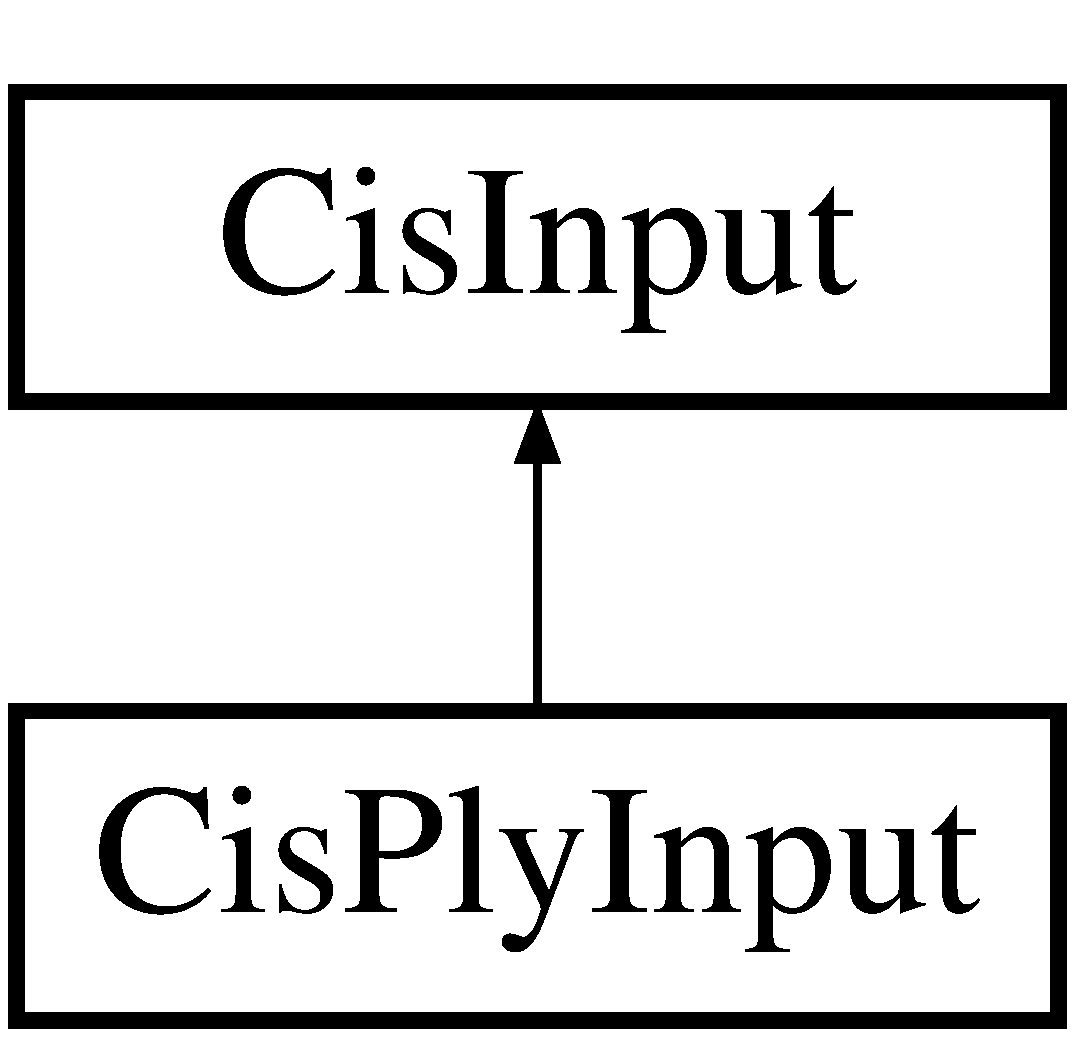
\includegraphics[height=2.000000cm]{classCisPlyInput}
\end{center}
\end{figure}
\subsection*{Public Member Functions}
\begin{DoxyCompactItemize}
\item 
\mbox{\hyperlink{classCisPlyInput_aedfc1d48a88199c0eb7b318f423b61c5}{Cis\+Ply\+Input}} (const char $\ast$name)
\begin{DoxyCompactList}\small\item\em Constructor for \mbox{\hyperlink{classCisPlyInput}{Cis\+Ply\+Input}}. \end{DoxyCompactList}\item 
\mbox{\Hypertarget{classCisPlyInput_ae44397567fdba765a43aba31af169fd0}\label{classCisPlyInput_ae44397567fdba765a43aba31af169fd0}} 
\mbox{\hyperlink{classCisPlyInput_ae44397567fdba765a43aba31af169fd0}{Cis\+Ply\+Input}} (cis\+Input\+\_\+t x)
\begin{DoxyCompactList}\small\item\em Empty constructor for inheritance. \end{DoxyCompactList}\end{DoxyCompactItemize}


\subsection{Detailed Description}
C++ interface to cis\+Ply\+Input\+\_\+t functionality. The \mbox{\hyperlink{classCisPlyInput}{Cis\+Ply\+Input}} class is a basic wrapper around the C cis\+Ply\+Input\+\_\+t structure and associated functions from the \mbox{\hyperlink{CisInterface_8h_source}{Cis\+Interface.\+h}} header. It provides the user with C++ style access to basic A\+S\+C\+II file input operations. 

\subsection{Constructor \& Destructor Documentation}
\mbox{\Hypertarget{classCisPlyInput_aedfc1d48a88199c0eb7b318f423b61c5}\label{classCisPlyInput_aedfc1d48a88199c0eb7b318f423b61c5}} 
\index{Cis\+Ply\+Input@{Cis\+Ply\+Input}!Cis\+Ply\+Input@{Cis\+Ply\+Input}}
\index{Cis\+Ply\+Input@{Cis\+Ply\+Input}!Cis\+Ply\+Input@{Cis\+Ply\+Input}}
\subsubsection{\texorpdfstring{Cis\+Ply\+Input()}{CisPlyInput()}}
{\footnotesize\ttfamily Cis\+Ply\+Input\+::\+Cis\+Ply\+Input (\begin{DoxyParamCaption}\item[{const char $\ast$}]{name }\end{DoxyParamCaption})\hspace{0.3cm}{\ttfamily [inline]}}



Constructor for \mbox{\hyperlink{classCisPlyInput}{Cis\+Ply\+Input}}. 


\begin{DoxyParams}[1]{Parameters}
\mbox{\tt in}  & {\em name} & constant character pointer to the name of an input channel. \\
\hline
\end{DoxyParams}


The documentation for this class was generated from the following file\+:\begin{DoxyCompactItemize}
\item 
/root/cis\+\_\+interface/cis\+\_\+interface/cis\+\_\+interface/interface/Cis\+Interface.\+hpp\end{DoxyCompactItemize}

\hypertarget{classCisPlyOutput}{}\section{Cis\+Ply\+Output Class Reference}
\label{classCisPlyOutput}\index{Cis\+Ply\+Output@{Cis\+Ply\+Output}}


C++ interface to cis\+Ply\+Output\+\_\+t functionality. The \mbox{\hyperlink{classCisPlyOutput}{Cis\+Ply\+Output}} class is a basic wrapper around the C cis\+Ply\+Output\+\_\+t structure and associated functions from the \mbox{\hyperlink{CisInterface_8h_source}{Cis\+Interface.\+h}} header. It provides the user with C++ style access to basic A\+S\+C\+II file output operations.  




{\ttfamily \#include $<$Cis\+Interface.\+hpp$>$}

Inheritance diagram for Cis\+Ply\+Output\+:\begin{figure}[H]
\begin{center}
\leavevmode
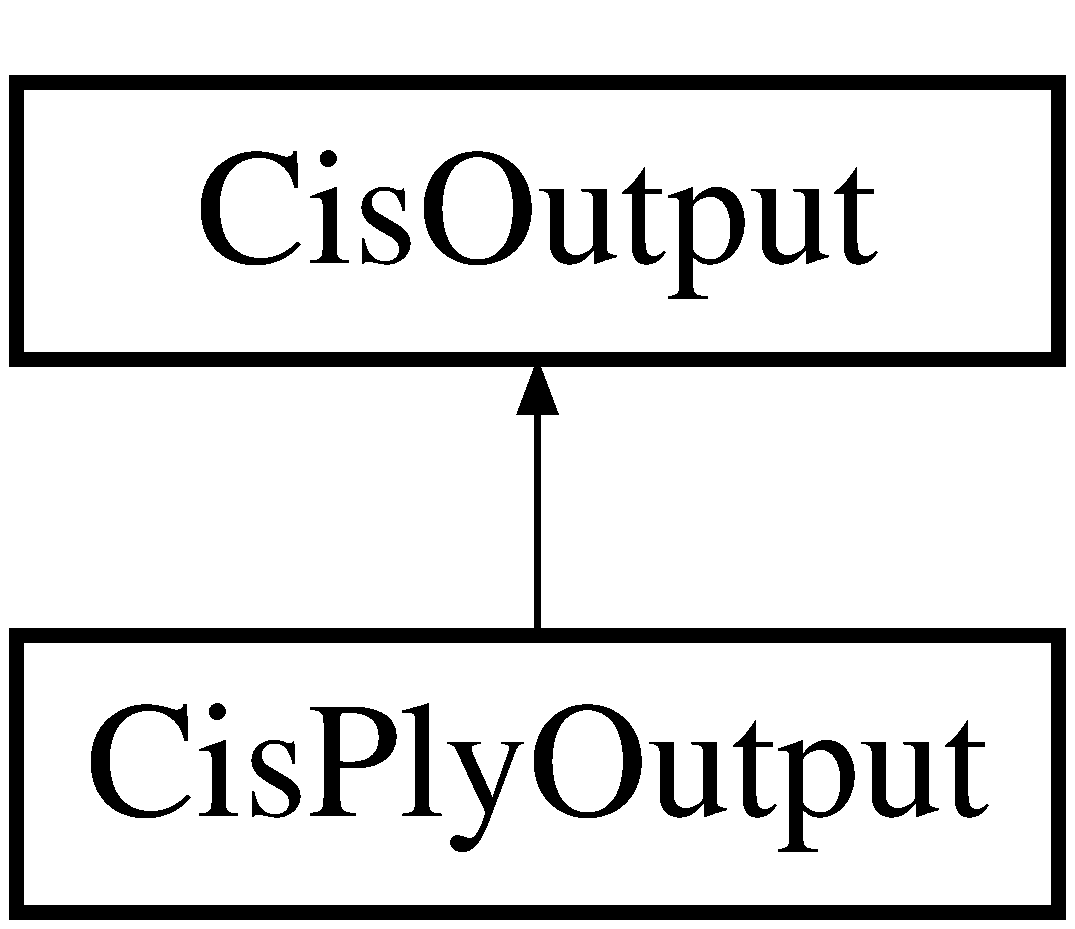
\includegraphics[height=2.000000cm]{classCisPlyOutput}
\end{center}
\end{figure}
\subsection*{Public Member Functions}
\begin{DoxyCompactItemize}
\item 
\mbox{\hyperlink{classCisPlyOutput_ae15d8b2786ee6353496795261861e840}{Cis\+Ply\+Output}} (const char $\ast$name)
\begin{DoxyCompactList}\small\item\em Constructor for \mbox{\hyperlink{classCisPlyOutput}{Cis\+Ply\+Output}}. \end{DoxyCompactList}\item 
\mbox{\Hypertarget{classCisPlyOutput_abf07624890d145e13a036b2b3640c134}\label{classCisPlyOutput_abf07624890d145e13a036b2b3640c134}} 
\mbox{\hyperlink{classCisPlyOutput_abf07624890d145e13a036b2b3640c134}{Cis\+Ply\+Output}} (cis\+Output\+\_\+t x)
\begin{DoxyCompactList}\small\item\em Empty constructor for inheritance. \end{DoxyCompactList}\end{DoxyCompactItemize}


\subsection{Detailed Description}
C++ interface to cis\+Ply\+Output\+\_\+t functionality. The \mbox{\hyperlink{classCisPlyOutput}{Cis\+Ply\+Output}} class is a basic wrapper around the C cis\+Ply\+Output\+\_\+t structure and associated functions from the \mbox{\hyperlink{CisInterface_8h_source}{Cis\+Interface.\+h}} header. It provides the user with C++ style access to basic A\+S\+C\+II file output operations. 

\subsection{Constructor \& Destructor Documentation}
\mbox{\Hypertarget{classCisPlyOutput_ae15d8b2786ee6353496795261861e840}\label{classCisPlyOutput_ae15d8b2786ee6353496795261861e840}} 
\index{Cis\+Ply\+Output@{Cis\+Ply\+Output}!Cis\+Ply\+Output@{Cis\+Ply\+Output}}
\index{Cis\+Ply\+Output@{Cis\+Ply\+Output}!Cis\+Ply\+Output@{Cis\+Ply\+Output}}
\subsubsection{\texorpdfstring{Cis\+Ply\+Output()}{CisPlyOutput()}}
{\footnotesize\ttfamily Cis\+Ply\+Output\+::\+Cis\+Ply\+Output (\begin{DoxyParamCaption}\item[{const char $\ast$}]{name }\end{DoxyParamCaption})\hspace{0.3cm}{\ttfamily [inline]}}



Constructor for \mbox{\hyperlink{classCisPlyOutput}{Cis\+Ply\+Output}}. 


\begin{DoxyParams}[1]{Parameters}
\mbox{\tt in}  & {\em name} & constant character pointer to the name of an output channel. \\
\hline
\end{DoxyParams}


The documentation for this class was generated from the following file\+:\begin{DoxyCompactItemize}
\item 
/root/cis\+\_\+interface/cis\+\_\+interface/cis\+\_\+interface/interface/Cis\+Interface.\+hpp\end{DoxyCompactItemize}

\hypertarget{classCisRpc}{}\section{Cis\+Rpc Class Reference}
\label{classCisRpc}\index{Cis\+Rpc@{Cis\+Rpc}}


C++ interface to cis\+Rpc\+\_\+t functionality.  




{\ttfamily \#include $<$Cis\+Interface.\+hpp$>$}

Inheritance diagram for Cis\+Rpc\+:\begin{figure}[H]
\begin{center}
\leavevmode
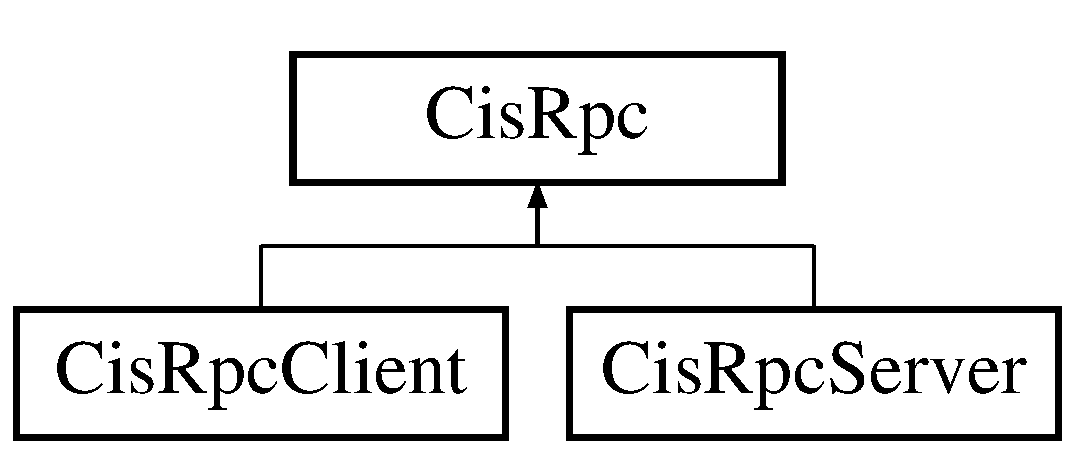
\includegraphics[height=2.000000cm]{classCisRpc}
\end{center}
\end{figure}
\subsection*{Public Member Functions}
\begin{DoxyCompactItemize}
\item 
\mbox{\hyperlink{classCisRpc_a91e65146ad3b4d1a3999835003b1cf37}{Cis\+Rpc}} (const char $\ast$name, const char $\ast$out\+Format, const char $\ast$in\+Format)
\begin{DoxyCompactList}\small\item\em Constructor for \mbox{\hyperlink{classCisRpc}{Cis\+Rpc}}. \end{DoxyCompactList}\item 
\mbox{\Hypertarget{classCisRpc_aca7fcde600dcb7b42ef93a5e9405358b}\label{classCisRpc_aca7fcde600dcb7b42ef93a5e9405358b}} 
\mbox{\hyperlink{classCisRpc_aca7fcde600dcb7b42ef93a5e9405358b}{Cis\+Rpc}} (cis\+Rpc\+\_\+t x)
\begin{DoxyCompactList}\small\item\em Empty constructor for inheritance. \end{DoxyCompactList}\item 
\mbox{\Hypertarget{classCisRpc_a29148e3e2924edc61aeec247ed939161}\label{classCisRpc_a29148e3e2924edc61aeec247ed939161}} 
void \mbox{\hyperlink{classCisRpc_a29148e3e2924edc61aeec247ed939161}{\+\_\+destroy\+\_\+pi}} ()
\begin{DoxyCompactList}\small\item\em Alias to allow freeing of underlying C struct at the class level. \end{DoxyCompactList}\item 
\mbox{\Hypertarget{classCisRpc_accbcccd1fd223660be6e8cf54cace2a8}\label{classCisRpc_accbcccd1fd223660be6e8cf54cace2a8}} 
\mbox{\hyperlink{classCisRpc_accbcccd1fd223660be6e8cf54cace2a8}{$\sim$\+Cis\+Rpc}} ()
\begin{DoxyCompactList}\small\item\em Destructor for \mbox{\hyperlink{classCisRpc}{Cis\+Rpc}}. See cis\+\_\+free in \mbox{\hyperlink{CisInterface_8h_source}{Cis\+Interface.\+h}} for details. \end{DoxyCompactList}\item 
cis\+Rpc\+\_\+t \mbox{\hyperlink{classCisRpc_ac58fc44e28ea378a1ef6b12684371aef}{pi}} ()
\begin{DoxyCompactList}\small\item\em Return the cis\+Rpc\+\_\+t structure. \end{DoxyCompactList}\item 
int \mbox{\hyperlink{classCisRpc_afb4143aa59acfe94df91435262cde01e}{send}} (const int nargs,...)
\begin{DoxyCompactList}\small\item\em Format and send a message to an R\+PC output queue. See rpc\+Send from \mbox{\hyperlink{CisInterface_8h_source}{Cis\+Interface.\+h}} for details. \end{DoxyCompactList}\item 
int \mbox{\hyperlink{classCisRpc_a6b1acb06791551c0c3096f678690e315}{recv}} (const int nargs,...)
\begin{DoxyCompactList}\small\item\em Receive and parse a message from an R\+PC input queue. See rpc\+Recv from \mbox{\hyperlink{CisInterface_8h_source}{Cis\+Interface.\+h}} for details. \end{DoxyCompactList}\end{DoxyCompactItemize}


\subsection{Detailed Description}
C++ interface to cis\+Rpc\+\_\+t functionality. 

The \mbox{\hyperlink{classCisRpc}{Cis\+Rpc}} class is a basic wrapper around the C cis\+Rpc\+\_\+t structure and associated functions from the \mbox{\hyperlink{CisInterface_8h_source}{Cis\+Interface.\+h}} header. It provides the user with C++ style access to basic R\+PC messaging via I\+PC queues. 

\subsection{Constructor \& Destructor Documentation}
\mbox{\Hypertarget{classCisRpc_a91e65146ad3b4d1a3999835003b1cf37}\label{classCisRpc_a91e65146ad3b4d1a3999835003b1cf37}} 
\index{Cis\+Rpc@{Cis\+Rpc}!Cis\+Rpc@{Cis\+Rpc}}
\index{Cis\+Rpc@{Cis\+Rpc}!Cis\+Rpc@{Cis\+Rpc}}
\subsubsection{\texorpdfstring{Cis\+Rpc()}{CisRpc()}}
{\footnotesize\ttfamily Cis\+Rpc\+::\+Cis\+Rpc (\begin{DoxyParamCaption}\item[{const char $\ast$}]{name,  }\item[{const char $\ast$}]{out\+Format,  }\item[{const char $\ast$}]{in\+Format }\end{DoxyParamCaption})\hspace{0.3cm}{\ttfamily [inline]}}



Constructor for \mbox{\hyperlink{classCisRpc}{Cis\+Rpc}}. 


\begin{DoxyParams}[1]{Parameters}
\mbox{\tt in}  & {\em name} & constant character pointer name of the output queue. \\
\hline
\mbox{\tt in}  & {\em out\+Format} & character pointer to format that should be used for formatting output. \\
\hline
\mbox{\tt in}  & {\em in\+Format} & character pointer to format that should be used for parsing input. \\
\hline
\end{DoxyParams}


\subsection{Member Function Documentation}
\mbox{\Hypertarget{classCisRpc_ac58fc44e28ea378a1ef6b12684371aef}\label{classCisRpc_ac58fc44e28ea378a1ef6b12684371aef}} 
\index{Cis\+Rpc@{Cis\+Rpc}!pi@{pi}}
\index{pi@{pi}!Cis\+Rpc@{Cis\+Rpc}}
\subsubsection{\texorpdfstring{pi()}{pi()}}
{\footnotesize\ttfamily cis\+Rpc\+\_\+t Cis\+Rpc\+::pi (\begin{DoxyParamCaption}{ }\end{DoxyParamCaption})\hspace{0.3cm}{\ttfamily [inline]}}



Return the cis\+Rpc\+\_\+t structure. 

\begin{DoxyReturn}{Returns}
cis\+Rpc\+\_\+t structure underlying the class. 
\end{DoxyReturn}
\mbox{\Hypertarget{classCisRpc_a6b1acb06791551c0c3096f678690e315}\label{classCisRpc_a6b1acb06791551c0c3096f678690e315}} 
\index{Cis\+Rpc@{Cis\+Rpc}!recv@{recv}}
\index{recv@{recv}!Cis\+Rpc@{Cis\+Rpc}}
\subsubsection{\texorpdfstring{recv()}{recv()}}
{\footnotesize\ttfamily int Cis\+Rpc\+::recv (\begin{DoxyParamCaption}\item[{const int}]{nargs,  }\item[{}]{... }\end{DoxyParamCaption})\hspace{0.3cm}{\ttfamily [inline]}}



Receive and parse a message from an R\+PC input queue. See rpc\+Recv from \mbox{\hyperlink{CisInterface_8h_source}{Cis\+Interface.\+h}} for details. 


\begin{DoxyParams}[1]{Parameters}
\mbox{\tt in}  & {\em nargs} & int Number of arguments being passed. \\
\hline
\mbox{\tt out}  & {\em ...} & mixed arguments that should be assigned parameters extracted using the format string. Since these will be assigned, they should be pointers to memory that has already been allocated. \\
\hline
\end{DoxyParams}
\begin{DoxyReturn}{Returns}
integer specifying if the receive was succesful. Values $>$= 0 indicate success. 
\end{DoxyReturn}
\mbox{\Hypertarget{classCisRpc_afb4143aa59acfe94df91435262cde01e}\label{classCisRpc_afb4143aa59acfe94df91435262cde01e}} 
\index{Cis\+Rpc@{Cis\+Rpc}!send@{send}}
\index{send@{send}!Cis\+Rpc@{Cis\+Rpc}}
\subsubsection{\texorpdfstring{send()}{send()}}
{\footnotesize\ttfamily int Cis\+Rpc\+::send (\begin{DoxyParamCaption}\item[{const int}]{nargs,  }\item[{}]{... }\end{DoxyParamCaption})\hspace{0.3cm}{\ttfamily [inline]}}



Format and send a message to an R\+PC output queue. See rpc\+Send from \mbox{\hyperlink{CisInterface_8h_source}{Cis\+Interface.\+h}} for details. 


\begin{DoxyParams}[1]{Parameters}
\mbox{\tt in}  & {\em nargs} & int Number of arguments being passed. \\
\hline
\mbox{\tt in}  & {\em ...} & arguments for formatting. ~\newline
\\
\hline
\end{DoxyParams}
\begin{DoxyReturn}{Returns}
integer specifying if the send was succesful. Values $>$= 0 indicate success. 
\end{DoxyReturn}


The documentation for this class was generated from the following file\+:\begin{DoxyCompactItemize}
\item 
/root/cis\+\_\+interface/cis\+\_\+interface/cis\+\_\+interface/interface/Cis\+Interface.\+hpp\end{DoxyCompactItemize}

\hypertarget{classCisRpcClient}{}\section{Cis\+Rpc\+Client Class Reference}
\label{classCisRpcClient}\index{Cis\+Rpc\+Client@{Cis\+Rpc\+Client}}


C++ interface to cis\+Rpc\+\_\+t client-\/side functionality. The \mbox{\hyperlink{classCisRpcClient}{Cis\+Rpc\+Client}} class is a basic wrapper around the C cis\+Rpc\+\_\+t structure and associated client-\/side functions from the \mbox{\hyperlink{CisInterface_8h_source}{Cis\+Interface.\+h}} header. It provides the user with C++ style access to basic R\+PC client operations.  




{\ttfamily \#include $<$Cis\+Interface.\+hpp$>$}

Inheritance diagram for Cis\+Rpc\+Client\+:\begin{figure}[H]
\begin{center}
\leavevmode
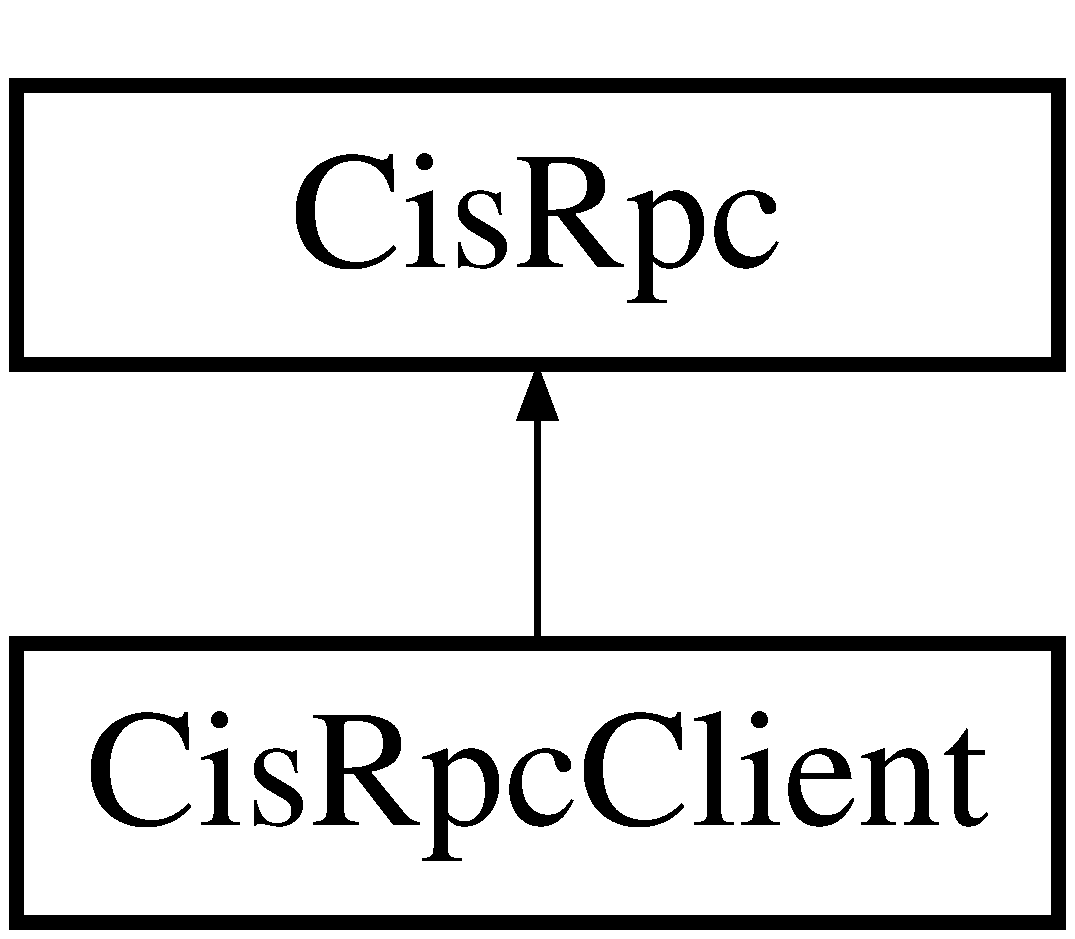
\includegraphics[height=2.000000cm]{classCisRpcClient}
\end{center}
\end{figure}
\subsection*{Public Member Functions}
\begin{DoxyCompactItemize}
\item 
\mbox{\hyperlink{classCisRpcClient_a02fb4a473e586bb441524365f976cc02}{Cis\+Rpc\+Client}} (const char $\ast$name, const char $\ast$out\+Format, const char $\ast$in\+Format)
\begin{DoxyCompactList}\small\item\em Constructor for \mbox{\hyperlink{classCisRpcClient}{Cis\+Rpc\+Client}}. \end{DoxyCompactList}\item 
\mbox{\Hypertarget{classCisRpcClient_a58598885fe23f219ab5d1b9f74ee1d6f}\label{classCisRpcClient_a58598885fe23f219ab5d1b9f74ee1d6f}} 
\mbox{\hyperlink{classCisRpcClient_a58598885fe23f219ab5d1b9f74ee1d6f}{$\sim$\+Cis\+Rpc\+Client}} ()
\begin{DoxyCompactList}\small\item\em Destructor for \mbox{\hyperlink{classCisRpcClient}{Cis\+Rpc\+Client}}. See cis\+\_\+free in \mbox{\hyperlink{CisInterface_8h_source}{Cis\+Interface.\+h}} for details. \end{DoxyCompactList}\item 
int \mbox{\hyperlink{classCisRpcClient_a2378157bcfdde78aef3f8a0068daec39}{call}} (const int nargs,...)
\begin{DoxyCompactList}\small\item\em Send request to an R\+PC server from the client and wait for a response. See rpc\+Call in \mbox{\hyperlink{CisInterface_8h_source}{Cis\+Interface.\+h}} for details. \end{DoxyCompactList}\end{DoxyCompactItemize}


\subsection{Detailed Description}
C++ interface to cis\+Rpc\+\_\+t client-\/side functionality. The \mbox{\hyperlink{classCisRpcClient}{Cis\+Rpc\+Client}} class is a basic wrapper around the C cis\+Rpc\+\_\+t structure and associated client-\/side functions from the \mbox{\hyperlink{CisInterface_8h_source}{Cis\+Interface.\+h}} header. It provides the user with C++ style access to basic R\+PC client operations. 

\subsection{Constructor \& Destructor Documentation}
\mbox{\Hypertarget{classCisRpcClient_a02fb4a473e586bb441524365f976cc02}\label{classCisRpcClient_a02fb4a473e586bb441524365f976cc02}} 
\index{Cis\+Rpc\+Client@{Cis\+Rpc\+Client}!Cis\+Rpc\+Client@{Cis\+Rpc\+Client}}
\index{Cis\+Rpc\+Client@{Cis\+Rpc\+Client}!Cis\+Rpc\+Client@{Cis\+Rpc\+Client}}
\subsubsection{\texorpdfstring{Cis\+Rpc\+Client()}{CisRpcClient()}}
{\footnotesize\ttfamily Cis\+Rpc\+Client\+::\+Cis\+Rpc\+Client (\begin{DoxyParamCaption}\item[{const char $\ast$}]{name,  }\item[{const char $\ast$}]{out\+Format,  }\item[{const char $\ast$}]{in\+Format }\end{DoxyParamCaption})\hspace{0.3cm}{\ttfamily [inline]}}



Constructor for \mbox{\hyperlink{classCisRpcClient}{Cis\+Rpc\+Client}}. 


\begin{DoxyParams}[1]{Parameters}
\mbox{\tt in}  & {\em name} & constant character pointer name used for input and output queues. \\
\hline
\mbox{\tt in}  & {\em out\+Format} & character pointer to format that should be used for formatting output. \\
\hline
\mbox{\tt in}  & {\em in\+Format} & character pointer to format that should be used for parsing input. \\
\hline
\end{DoxyParams}


\subsection{Member Function Documentation}
\mbox{\Hypertarget{classCisRpcClient_a2378157bcfdde78aef3f8a0068daec39}\label{classCisRpcClient_a2378157bcfdde78aef3f8a0068daec39}} 
\index{Cis\+Rpc\+Client@{Cis\+Rpc\+Client}!call@{call}}
\index{call@{call}!Cis\+Rpc\+Client@{Cis\+Rpc\+Client}}
\subsubsection{\texorpdfstring{call()}{call()}}
{\footnotesize\ttfamily int Cis\+Rpc\+Client\+::call (\begin{DoxyParamCaption}\item[{const int}]{nargs,  }\item[{}]{... }\end{DoxyParamCaption})\hspace{0.3cm}{\ttfamily [inline]}}



Send request to an R\+PC server from the client and wait for a response. See rpc\+Call in \mbox{\hyperlink{CisInterface_8h_source}{Cis\+Interface.\+h}} for details. 


\begin{DoxyParams}[1]{Parameters}
\mbox{\tt in}  & {\em nargs} & int Number of arguments being passed. \\
\hline
\mbox{\tt in,out}  & {\em ...} & mixed arguments that include those that should be formatted using the output format string, followed by those that should be assigned parameters extracted using the input format string. These that will be assigned should be pointers to memory that has already been allocated. \\
\hline
\end{DoxyParams}
\begin{DoxyReturn}{Returns}
integer specifying if the receive was succesful. Values $>$= 0 indicate success. 
\end{DoxyReturn}


The documentation for this class was generated from the following file\+:\begin{DoxyCompactItemize}
\item 
/root/cis\+\_\+interface/cis\+\_\+interface/cis\+\_\+interface/interface/Cis\+Interface.\+hpp\end{DoxyCompactItemize}

\hypertarget{classCisRpcServer}{}\section{Cis\+Rpc\+Server Class Reference}
\label{classCisRpcServer}\index{Cis\+Rpc\+Server@{Cis\+Rpc\+Server}}


C++ interface to cis\+Rpc\+\_\+t server-\/side functionality. The \mbox{\hyperlink{classCisRpcServer}{Cis\+Rpc\+Server}} class is a basic wrapper around the C cis\+Rpc\+\_\+t structure and associated server-\/side functions from the \mbox{\hyperlink{CisInterface_8h_source}{Cis\+Interface.\+h}} header. It provides the user with C++ style access to basic R\+PC server operations.  




{\ttfamily \#include $<$Cis\+Interface.\+hpp$>$}

Inheritance diagram for Cis\+Rpc\+Server\+:\begin{figure}[H]
\begin{center}
\leavevmode
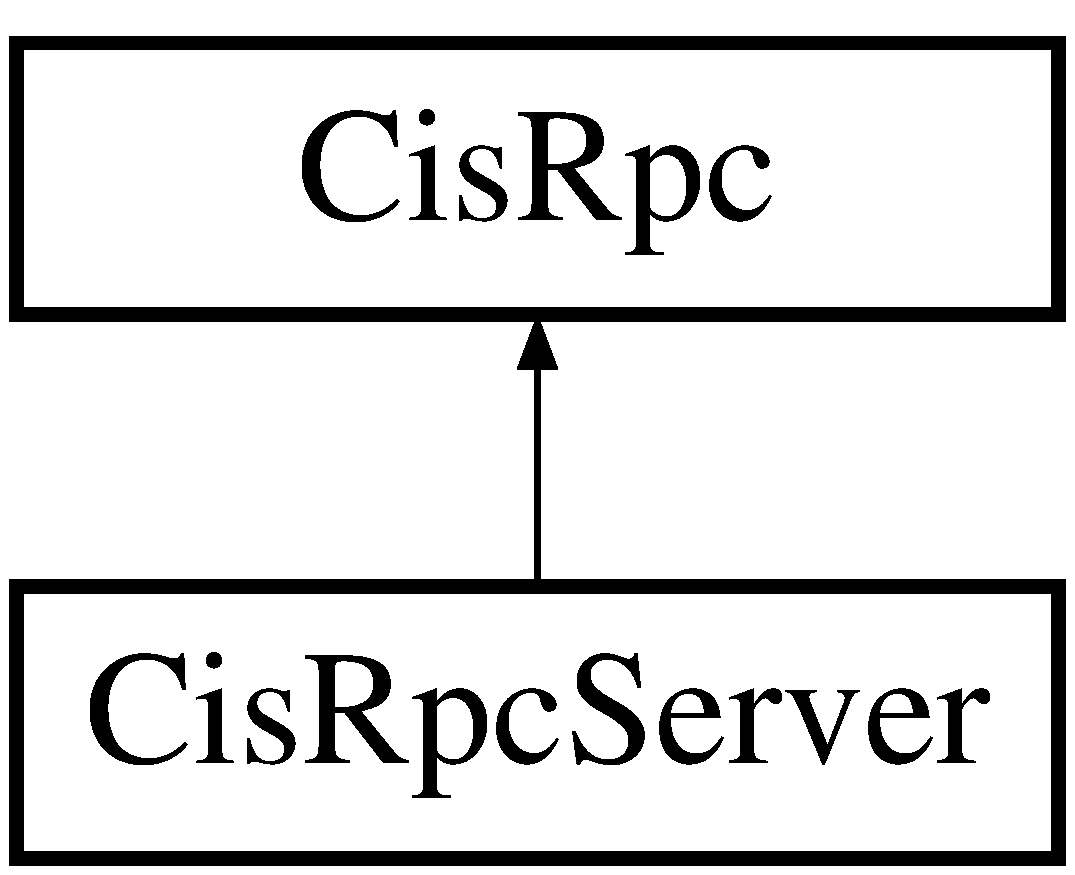
\includegraphics[height=2.000000cm]{classCisRpcServer}
\end{center}
\end{figure}
\subsection*{Public Member Functions}
\begin{DoxyCompactItemize}
\item 
\mbox{\hyperlink{classCisRpcServer_a4d531d6b97d3916f9b4fe9398b71f60f}{Cis\+Rpc\+Server}} (const char $\ast$name, const char $\ast$in\+Format, const char $\ast$out\+Format)
\begin{DoxyCompactList}\small\item\em Constructor for \mbox{\hyperlink{classCisRpcServer}{Cis\+Rpc\+Server}}. \end{DoxyCompactList}\item 
\mbox{\Hypertarget{classCisRpcServer_a5681ecdcbcd03ad613f4843c39a3403b}\label{classCisRpcServer_a5681ecdcbcd03ad613f4843c39a3403b}} 
\mbox{\hyperlink{classCisRpcServer_a5681ecdcbcd03ad613f4843c39a3403b}{$\sim$\+Cis\+Rpc\+Server}} ()
\begin{DoxyCompactList}\small\item\em Destructor for \mbox{\hyperlink{classCisRpcServer}{Cis\+Rpc\+Server}}. See cis\+\_\+free in \mbox{\hyperlink{CisInterface_8h_source}{Cis\+Interface.\+h}} for details. \end{DoxyCompactList}\end{DoxyCompactItemize}


\subsection{Detailed Description}
C++ interface to cis\+Rpc\+\_\+t server-\/side functionality. The \mbox{\hyperlink{classCisRpcServer}{Cis\+Rpc\+Server}} class is a basic wrapper around the C cis\+Rpc\+\_\+t structure and associated server-\/side functions from the \mbox{\hyperlink{CisInterface_8h_source}{Cis\+Interface.\+h}} header. It provides the user with C++ style access to basic R\+PC server operations. 

\subsection{Constructor \& Destructor Documentation}
\mbox{\Hypertarget{classCisRpcServer_a4d531d6b97d3916f9b4fe9398b71f60f}\label{classCisRpcServer_a4d531d6b97d3916f9b4fe9398b71f60f}} 
\index{Cis\+Rpc\+Server@{Cis\+Rpc\+Server}!Cis\+Rpc\+Server@{Cis\+Rpc\+Server}}
\index{Cis\+Rpc\+Server@{Cis\+Rpc\+Server}!Cis\+Rpc\+Server@{Cis\+Rpc\+Server}}
\subsubsection{\texorpdfstring{Cis\+Rpc\+Server()}{CisRpcServer()}}
{\footnotesize\ttfamily Cis\+Rpc\+Server\+::\+Cis\+Rpc\+Server (\begin{DoxyParamCaption}\item[{const char $\ast$}]{name,  }\item[{const char $\ast$}]{in\+Format,  }\item[{const char $\ast$}]{out\+Format }\end{DoxyParamCaption})\hspace{0.3cm}{\ttfamily [inline]}}



Constructor for \mbox{\hyperlink{classCisRpcServer}{Cis\+Rpc\+Server}}. 


\begin{DoxyParams}[1]{Parameters}
\mbox{\tt in}  & {\em name} & constant character pointer name used for input and output queues. \\
\hline
\mbox{\tt in}  & {\em in\+Format} & character pointer to format that should be used for parsing input. \\
\hline
\mbox{\tt in}  & {\em out\+Format} & character pointer to format that should be used for formatting output. \\
\hline
\end{DoxyParams}


The documentation for this class was generated from the following file\+:\begin{DoxyCompactItemize}
\item 
/root/cis\+\_\+interface/cis\+\_\+interface/cis\+\_\+interface/interface/Cis\+Interface.\+hpp\end{DoxyCompactItemize}

\hypertarget{structcomm__head__t}{}\section{comm\+\_\+head\+\_\+t Struct Reference}
\label{structcomm__head__t}\index{comm\+\_\+head\+\_\+t@{comm\+\_\+head\+\_\+t}}


Header information passed by comms for multipart messages.  




{\ttfamily \#include $<$comm\+\_\+header.\+h$>$}

\subsection*{Public Attributes}
\begin{DoxyCompactItemize}
\item 
\mbox{\Hypertarget{structcomm__head__t_a61721f46c3f5850a5e65e28d497da0fb}\label{structcomm__head__t_a61721f46c3f5850a5e65e28d497da0fb}} 
size\+\_\+t \mbox{\hyperlink{structcomm__head__t_a61721f46c3f5850a5e65e28d497da0fb}{size}}
\begin{DoxyCompactList}\small\item\em Size of incoming message. \end{DoxyCompactList}\item 
\mbox{\Hypertarget{structcomm__head__t_af762f3a390be988bb2f9dca01a7b5bb5}\label{structcomm__head__t_af762f3a390be988bb2f9dca01a7b5bb5}} 
char \mbox{\hyperlink{structcomm__head__t_af762f3a390be988bb2f9dca01a7b5bb5}{address}} \mbox{[}C\+O\+M\+M\+B\+U\+F\+F\+S\+IZ\mbox{]}
\begin{DoxyCompactList}\small\item\em Address that message will comm in on. \end{DoxyCompactList}\item 
\mbox{\Hypertarget{structcomm__head__t_a6f14ffcda4738e5e4b498b05a802f293}\label{structcomm__head__t_a6f14ffcda4738e5e4b498b05a802f293}} 
int \mbox{\hyperlink{structcomm__head__t_a6f14ffcda4738e5e4b498b05a802f293}{multipart}}
\begin{DoxyCompactList}\small\item\em 1 if message is multipart, 0 if it is not. \end{DoxyCompactList}\item 
\mbox{\Hypertarget{structcomm__head__t_a981bda83ada0637a0153dcd6c46420f0}\label{structcomm__head__t_a981bda83ada0637a0153dcd6c46420f0}} 
size\+\_\+t \mbox{\hyperlink{structcomm__head__t_a981bda83ada0637a0153dcd6c46420f0}{bodysiz}}
\begin{DoxyCompactList}\small\item\em Size of body. \end{DoxyCompactList}\item 
\mbox{\Hypertarget{structcomm__head__t_a5e01ad7e302f5597bccfcf208cdcbe0a}\label{structcomm__head__t_a5e01ad7e302f5597bccfcf208cdcbe0a}} 
size\+\_\+t \mbox{\hyperlink{structcomm__head__t_a5e01ad7e302f5597bccfcf208cdcbe0a}{bodybeg}}
\begin{DoxyCompactList}\small\item\em Start of body in header. \end{DoxyCompactList}\item 
\mbox{\Hypertarget{structcomm__head__t_a541f991a66b2422bec7b1cc25b5dd567}\label{structcomm__head__t_a541f991a66b2422bec7b1cc25b5dd567}} 
int \mbox{\hyperlink{structcomm__head__t_a541f991a66b2422bec7b1cc25b5dd567}{valid}}
\begin{DoxyCompactList}\small\item\em 1 if the header is valid, 0 otherwise. \end{DoxyCompactList}\item 
\mbox{\Hypertarget{structcomm__head__t_ade03bb53d07aaffff906db9a8d95da02}\label{structcomm__head__t_ade03bb53d07aaffff906db9a8d95da02}} 
char \mbox{\hyperlink{structcomm__head__t_ade03bb53d07aaffff906db9a8d95da02}{id}} \mbox{[}C\+O\+M\+M\+B\+U\+F\+F\+S\+IZ\mbox{]}
\begin{DoxyCompactList}\small\item\em Unique ID associated with this message. \end{DoxyCompactList}\item 
\mbox{\Hypertarget{structcomm__head__t_a5a1970e9fb2c1087c001345603ab5c2b}\label{structcomm__head__t_a5a1970e9fb2c1087c001345603ab5c2b}} 
char \mbox{\hyperlink{structcomm__head__t_a5a1970e9fb2c1087c001345603ab5c2b}{response\+\_\+address}} \mbox{[}C\+O\+M\+M\+B\+U\+F\+F\+S\+IZ\mbox{]}
\begin{DoxyCompactList}\small\item\em Response address. \end{DoxyCompactList}\item 
\mbox{\Hypertarget{structcomm__head__t_a80b9979899d06f21b7f996c1a119e665}\label{structcomm__head__t_a80b9979899d06f21b7f996c1a119e665}} 
char \mbox{\hyperlink{structcomm__head__t_a80b9979899d06f21b7f996c1a119e665}{request\+\_\+id}} \mbox{[}C\+O\+M\+M\+B\+U\+F\+F\+S\+IZ\mbox{]}
\begin{DoxyCompactList}\small\item\em Request id. \end{DoxyCompactList}\item 
\mbox{\Hypertarget{structcomm__head__t_a4d963ff774cc3537d8944856b2365c6a}\label{structcomm__head__t_a4d963ff774cc3537d8944856b2365c6a}} 
int \mbox{\hyperlink{structcomm__head__t_a4d963ff774cc3537d8944856b2365c6a}{serializer\+\_\+type}}
\begin{DoxyCompactList}\small\item\em Code indicating the type of serializer. \end{DoxyCompactList}\item 
\mbox{\Hypertarget{structcomm__head__t_acfddb7dfc30cd546036af32cab2295e2}\label{structcomm__head__t_acfddb7dfc30cd546036af32cab2295e2}} 
char \mbox{\hyperlink{structcomm__head__t_acfddb7dfc30cd546036af32cab2295e2}{format\+\_\+str}} \mbox{[}C\+O\+M\+M\+B\+U\+F\+F\+S\+IZ\mbox{]}
\begin{DoxyCompactList}\small\item\em Format string for serializer. \end{DoxyCompactList}\item 
\mbox{\Hypertarget{structcomm__head__t_a15efa818f71d8712b6f3270ca3c45ef1}\label{structcomm__head__t_a15efa818f71d8712b6f3270ca3c45ef1}} 
char \mbox{\hyperlink{structcomm__head__t_a15efa818f71d8712b6f3270ca3c45ef1}{field\+\_\+names}} \mbox{[}C\+O\+M\+M\+B\+U\+F\+F\+S\+IZ\mbox{]}
\begin{DoxyCompactList}\small\item\em String containing field names. \end{DoxyCompactList}\item 
\mbox{\Hypertarget{structcomm__head__t_ac2d45e0c1ac6a748e1516bfac30f359b}\label{structcomm__head__t_ac2d45e0c1ac6a748e1516bfac30f359b}} 
char \mbox{\hyperlink{structcomm__head__t_ac2d45e0c1ac6a748e1516bfac30f359b}{field\+\_\+units}} \mbox{[}C\+O\+M\+M\+B\+U\+F\+F\+S\+IZ\mbox{]}
\begin{DoxyCompactList}\small\item\em String containing field units. \end{DoxyCompactList}\item 
\mbox{\Hypertarget{structcomm__head__t_a68f4fd55f648414958edcd564be498b7}\label{structcomm__head__t_a68f4fd55f648414958edcd564be498b7}} 
int \mbox{\hyperlink{structcomm__head__t_a68f4fd55f648414958edcd564be498b7}{as\+\_\+array}}
\begin{DoxyCompactList}\small\item\em 1 if messages will be serialized arrays. \end{DoxyCompactList}\item 
\mbox{\Hypertarget{structcomm__head__t_a81034ab274964279115f5ce7669f055b}\label{structcomm__head__t_a81034ab274964279115f5ce7669f055b}} 
char \mbox{\hyperlink{structcomm__head__t_a81034ab274964279115f5ce7669f055b}{zmq\+\_\+reply}} \mbox{[}C\+O\+M\+M\+B\+U\+F\+F\+S\+IZ\mbox{]}
\begin{DoxyCompactList}\small\item\em Reply address for Z\+MQ sockets. \end{DoxyCompactList}\item 
\mbox{\Hypertarget{structcomm__head__t_a1367a9bb9ef1938d87897ab5685b01ef}\label{structcomm__head__t_a1367a9bb9ef1938d87897ab5685b01ef}} 
char \mbox{\hyperlink{structcomm__head__t_a1367a9bb9ef1938d87897ab5685b01ef}{zmq\+\_\+reply\+\_\+worker}} \mbox{[}C\+O\+M\+M\+B\+U\+F\+F\+S\+IZ\mbox{]}
\begin{DoxyCompactList}\small\item\em Reply address for worker socket. \end{DoxyCompactList}\end{DoxyCompactItemize}


\subsection{Detailed Description}
Header information passed by comms for multipart messages. 

The documentation for this struct was generated from the following file\+:\begin{DoxyCompactItemize}
\item 
/root/cis\+\_\+interface/cis\+\_\+interface/cis\+\_\+interface/communication/comm\+\_\+header.\+h\end{DoxyCompactItemize}

\hypertarget{structcomm__t}{}\section{comm\+\_\+t Struct Reference}
\label{structcomm__t}\index{comm\+\_\+t@{comm\+\_\+t}}


Communication structure.  




{\ttfamily \#include $<$Comm\+Base.\+h$>$}

\subsection*{Public Attributes}
\begin{DoxyCompactItemize}
\item 
\mbox{\Hypertarget{structcomm__t_a9bd691f3ae56e098b9edff7ad1628b3b}\label{structcomm__t_a9bd691f3ae56e098b9edff7ad1628b3b}} 
comm\+\_\+type \mbox{\hyperlink{structcomm__t_a9bd691f3ae56e098b9edff7ad1628b3b}{type}}
\begin{DoxyCompactList}\small\item\em Comm type. \end{DoxyCompactList}\item 
\mbox{\Hypertarget{structcomm__t_a0c8b237f48a50a181eab8447a87ec172}\label{structcomm__t_a0c8b237f48a50a181eab8447a87ec172}} 
char \mbox{\hyperlink{structcomm__t_a0c8b237f48a50a181eab8447a87ec172}{name}} \mbox{[}C\+O\+M\+M\+\_\+\+N\+A\+M\+E\+\_\+\+S\+I\+ZE\mbox{]}
\begin{DoxyCompactList}\small\item\em Comm name. \end{DoxyCompactList}\item 
\mbox{\Hypertarget{structcomm__t_aca2bf1fc2b62c779c50848501f31fbf0}\label{structcomm__t_aca2bf1fc2b62c779c50848501f31fbf0}} 
char \mbox{\hyperlink{structcomm__t_aca2bf1fc2b62c779c50848501f31fbf0}{address}} \mbox{[}C\+O\+M\+M\+\_\+\+A\+D\+D\+R\+E\+S\+S\+\_\+\+S\+I\+ZE\mbox{]}
\begin{DoxyCompactList}\small\item\em Comm address. \end{DoxyCompactList}\item 
\mbox{\Hypertarget{structcomm__t_a1940bbad161f8cf5f868ff4cf4e95cda}\label{structcomm__t_a1940bbad161f8cf5f868ff4cf4e95cda}} 
char \mbox{\hyperlink{structcomm__t_a1940bbad161f8cf5f868ff4cf4e95cda}{direction}} \mbox{[}C\+O\+M\+M\+\_\+\+D\+I\+R\+\_\+\+S\+I\+ZE\mbox{]}
\begin{DoxyCompactList}\small\item\em send or recv for direction messages will go. \end{DoxyCompactList}\item 
\mbox{\Hypertarget{structcomm__t_afe8a58007e764fb3f2e906025f89fe72}\label{structcomm__t_afe8a58007e764fb3f2e906025f89fe72}} 
int \mbox{\hyperlink{structcomm__t_afe8a58007e764fb3f2e906025f89fe72}{valid}}
\begin{DoxyCompactList}\small\item\em 1 if communicator initialized, 0 otherwise. \end{DoxyCompactList}\item 
\mbox{\Hypertarget{structcomm__t_ab7b58a54178acddc3f641e3a285aab7f}\label{structcomm__t_ab7b58a54178acddc3f641e3a285aab7f}} 
void $\ast$ \mbox{\hyperlink{structcomm__t_ab7b58a54178acddc3f641e3a285aab7f}{handle}}
\begin{DoxyCompactList}\small\item\em Pointer to handle for comm. \end{DoxyCompactList}\item 
\mbox{\Hypertarget{structcomm__t_ac805f6f060d8a6d7be78e9e782d15fdd}\label{structcomm__t_ac805f6f060d8a6d7be78e9e782d15fdd}} 
void $\ast$ \mbox{\hyperlink{structcomm__t_ac805f6f060d8a6d7be78e9e782d15fdd}{info}}
\begin{DoxyCompactList}\small\item\em Pointer to any extra info comm requires. \end{DoxyCompactList}\item 
\mbox{\Hypertarget{structcomm__t_a2c1ca12d0df5193d4a023301aa156e8f}\label{structcomm__t_a2c1ca12d0df5193d4a023301aa156e8f}} 
\mbox{\hyperlink{structseri__t}{seri\+\_\+t}} $\ast$ \mbox{\hyperlink{structcomm__t_a2c1ca12d0df5193d4a023301aa156e8f}{serializer}}
\begin{DoxyCompactList}\small\item\em Serializer for comm messages. \end{DoxyCompactList}\item 
\mbox{\Hypertarget{structcomm__t_a9aecec459dff6ce20398f1c110f8f3f4}\label{structcomm__t_a9aecec459dff6ce20398f1c110f8f3f4}} 
size\+\_\+t \mbox{\hyperlink{structcomm__t_a9aecec459dff6ce20398f1c110f8f3f4}{max\+Msg\+Size}}
\begin{DoxyCompactList}\small\item\em The maximum message size. \end{DoxyCompactList}\item 
\mbox{\Hypertarget{structcomm__t_a9810578a787d8503b00bcb78a592073d}\label{structcomm__t_a9810578a787d8503b00bcb78a592073d}} 
int \mbox{\hyperlink{structcomm__t_a9810578a787d8503b00bcb78a592073d}{always\+\_\+send\+\_\+header}}
\begin{DoxyCompactList}\small\item\em 1 if comm should always send a header. \end{DoxyCompactList}\item 
\mbox{\Hypertarget{structcomm__t_a87f3a39926576e049b9ddc0cbabc9c95}\label{structcomm__t_a87f3a39926576e049b9ddc0cbabc9c95}} 
int \mbox{\hyperlink{structcomm__t_a87f3a39926576e049b9ddc0cbabc9c95}{index\+\_\+in\+\_\+register}}
\begin{DoxyCompactList}\small\item\em Index of the comm in the comm register. \end{DoxyCompactList}\item 
\mbox{\Hypertarget{structcomm__t_adc0fcb148259e9801f63e70f7945e31b}\label{structcomm__t_adc0fcb148259e9801f63e70f7945e31b}} 
time\+\_\+t $\ast$ \mbox{\hyperlink{structcomm__t_adc0fcb148259e9801f63e70f7945e31b}{last\+\_\+send}}
\begin{DoxyCompactList}\small\item\em Clock output at time of last send. \end{DoxyCompactList}\item 
\mbox{\Hypertarget{structcomm__t_a9c883133ed0ee04e11983dc7efbc8bfb}\label{structcomm__t_a9c883133ed0ee04e11983dc7efbc8bfb}} 
int $\ast$ \mbox{\hyperlink{structcomm__t_a9c883133ed0ee04e11983dc7efbc8bfb}{sent\+\_\+eof}}
\begin{DoxyCompactList}\small\item\em Flag specifying if E\+OF has been sent. \end{DoxyCompactList}\item 
\mbox{\Hypertarget{structcomm__t_a1d7418e5f54be56939a7f26b68a55f3d}\label{structcomm__t_a1d7418e5f54be56939a7f26b68a55f3d}} 
int $\ast$ \mbox{\hyperlink{structcomm__t_a1d7418e5f54be56939a7f26b68a55f3d}{recv\+\_\+eof}}
\begin{DoxyCompactList}\small\item\em Flag specifying if E\+OF has been received. \end{DoxyCompactList}\item 
\mbox{\Hypertarget{structcomm__t_a7a90d80ee6c1826d0fc152dc3a3f61a1}\label{structcomm__t_a7a90d80ee6c1826d0fc152dc3a3f61a1}} 
int $\ast$ \mbox{\hyperlink{structcomm__t_a7a90d80ee6c1826d0fc152dc3a3f61a1}{used}}
\begin{DoxyCompactList}\small\item\em Flag specifying if the comm has been used. \end{DoxyCompactList}\item 
\mbox{\Hypertarget{structcomm__t_a05095fa4451ed9085e2d23bb5304df10}\label{structcomm__t_a05095fa4451ed9085e2d23bb5304df10}} 
void $\ast$ \mbox{\hyperlink{structcomm__t_a05095fa4451ed9085e2d23bb5304df10}{reply}}
\begin{DoxyCompactList}\small\item\em Reply information. \end{DoxyCompactList}\item 
\mbox{\Hypertarget{structcomm__t_a2d004dd7203d970ac2f398a25276ad2f}\label{structcomm__t_a2d004dd7203d970ac2f398a25276ad2f}} 
int \mbox{\hyperlink{structcomm__t_a2d004dd7203d970ac2f398a25276ad2f}{is\+\_\+file}}
\begin{DoxyCompactList}\small\item\em Flag specifying if the comm connects directly to a file. \end{DoxyCompactList}\item 
\mbox{\Hypertarget{structcomm__t_a9b44169ff04756e8802bb2510892cf56}\label{structcomm__t_a9b44169ff04756e8802bb2510892cf56}} 
int \mbox{\hyperlink{structcomm__t_a9b44169ff04756e8802bb2510892cf56}{is\+\_\+work\+\_\+comm}}
\begin{DoxyCompactList}\small\item\em Flag specifying if comm is a temporary work comm. \end{DoxyCompactList}\end{DoxyCompactItemize}


\subsection{Detailed Description}
Communication structure. 

The documentation for this struct was generated from the following file\+:\begin{DoxyCompactItemize}
\item 
/root/cis\+\_\+interface/cis\+\_\+interface/cis\+\_\+interface/communication/Comm\+Base.\+h\end{DoxyCompactItemize}

\hypertarget{structobj__t}{}\section{obj\+\_\+t Struct Reference}
\label{structobj__t}\index{obj\+\_\+t@{obj\+\_\+t}}


Obj structure.  




{\ttfamily \#include $<$Obj\+Serialize.\+h$>$}

\subsection*{Public Attributes}
\begin{DoxyCompactItemize}
\item 
\mbox{\Hypertarget{structobj__t_aa08e8272f5b5f143afac1cab58d30518}\label{structobj__t_aa08e8272f5b5f143afac1cab58d30518}} 
int \mbox{\hyperlink{structobj__t_aa08e8272f5b5f143afac1cab58d30518}{nvert}}
\begin{DoxyCompactList}\small\item\em Number of vertices. \end{DoxyCompactList}\item 
\mbox{\Hypertarget{structobj__t_a28c4194c71f1cd6c719f43c70ee14df6}\label{structobj__t_a28c4194c71f1cd6c719f43c70ee14df6}} 
int \mbox{\hyperlink{structobj__t_a28c4194c71f1cd6c719f43c70ee14df6}{nface}}
\begin{DoxyCompactList}\small\item\em Number faces. \end{DoxyCompactList}\item 
\mbox{\Hypertarget{structobj__t_a57882cfdbfe09ad7b4a5fcede3681b6b}\label{structobj__t_a57882cfdbfe09ad7b4a5fcede3681b6b}} 
float $\ast$$\ast$ \mbox{\hyperlink{structobj__t_a57882cfdbfe09ad7b4a5fcede3681b6b}{vertices}}
\begin{DoxyCompactList}\small\item\em X, Y, Z positions of vertices. \end{DoxyCompactList}\item 
\mbox{\Hypertarget{structobj__t_a450705239dad767420e27d4bb2b1a7cb}\label{structobj__t_a450705239dad767420e27d4bb2b1a7cb}} 
int $\ast$$\ast$ \mbox{\hyperlink{structobj__t_a450705239dad767420e27d4bb2b1a7cb}{faces}}
\begin{DoxyCompactList}\small\item\em Indices of the vertices composing each face. \end{DoxyCompactList}\item 
\mbox{\Hypertarget{structobj__t_a26c45b63e6ff01ff6f9f1d5f25bb7d0b}\label{structobj__t_a26c45b63e6ff01ff6f9f1d5f25bb7d0b}} 
int $\ast$$\ast$ \mbox{\hyperlink{structobj__t_a26c45b63e6ff01ff6f9f1d5f25bb7d0b}{vertex\+\_\+colors}}
\begin{DoxyCompactList}\small\item\em R\+GB colors of each vertex. \end{DoxyCompactList}\item 
\mbox{\Hypertarget{structobj__t_ac8ff1d64bfbec1df635bf72ba7fd5486}\label{structobj__t_ac8ff1d64bfbec1df635bf72ba7fd5486}} 
char \mbox{\hyperlink{structobj__t_ac8ff1d64bfbec1df635bf72ba7fd5486}{material}} \mbox{[}100\mbox{]}
\begin{DoxyCompactList}\small\item\em Material that should be used for faces. \end{DoxyCompactList}\item 
\mbox{\Hypertarget{structobj__t_aaa36aa6eda039139d79a807b591d1a1a}\label{structobj__t_aaa36aa6eda039139d79a807b591d1a1a}} 
int \mbox{\hyperlink{structobj__t_aaa36aa6eda039139d79a807b591d1a1a}{ntexc}}
\begin{DoxyCompactList}\small\item\em Number of texture coordinates. \end{DoxyCompactList}\item 
\mbox{\Hypertarget{structobj__t_aeaae61787b92ea57ef185bdd9e996b02}\label{structobj__t_aeaae61787b92ea57ef185bdd9e996b02}} 
int \mbox{\hyperlink{structobj__t_aeaae61787b92ea57ef185bdd9e996b02}{nnorm}}
\begin{DoxyCompactList}\small\item\em Number of normals. \end{DoxyCompactList}\item 
\mbox{\Hypertarget{structobj__t_a9477aca6c3d6977280f1082410576438}\label{structobj__t_a9477aca6c3d6977280f1082410576438}} 
float $\ast$$\ast$ \mbox{\hyperlink{structobj__t_a9477aca6c3d6977280f1082410576438}{texcoords}}
\begin{DoxyCompactList}\small\item\em Texture coordinates. \end{DoxyCompactList}\item 
\mbox{\Hypertarget{structobj__t_ac61278759dc377f187ce6ae7c8b3c668}\label{structobj__t_ac61278759dc377f187ce6ae7c8b3c668}} 
float $\ast$$\ast$ \mbox{\hyperlink{structobj__t_ac61278759dc377f187ce6ae7c8b3c668}{normals}}
\begin{DoxyCompactList}\small\item\em X, Y, Z direction of normals. \end{DoxyCompactList}\item 
\mbox{\Hypertarget{structobj__t_a06e3e2f89a4bd511413240569bd3f98e}\label{structobj__t_a06e3e2f89a4bd511413240569bd3f98e}} 
int $\ast$$\ast$ \mbox{\hyperlink{structobj__t_a06e3e2f89a4bd511413240569bd3f98e}{face\+\_\+texcoords}}
\begin{DoxyCompactList}\small\item\em Indices of texcoords for each face. \end{DoxyCompactList}\item 
\mbox{\Hypertarget{structobj__t_ae48ff9d93e071669d7b6edccb7aaf642}\label{structobj__t_ae48ff9d93e071669d7b6edccb7aaf642}} 
int $\ast$$\ast$ \mbox{\hyperlink{structobj__t_ae48ff9d93e071669d7b6edccb7aaf642}{face\+\_\+normals}}
\begin{DoxyCompactList}\small\item\em Indices of normals for each face. \end{DoxyCompactList}\end{DoxyCompactItemize}


\subsection{Detailed Description}
Obj structure. 

The documentation for this struct was generated from the following file\+:\begin{DoxyCompactItemize}
\item 
/root/cis\+\_\+interface/cis\+\_\+interface/cis\+\_\+interface/serialize/Obj\+Serialize.\+h\end{DoxyCompactItemize}

\hypertarget{structply__t}{}\section{ply\+\_\+t Struct Reference}
\label{structply__t}\index{ply\+\_\+t@{ply\+\_\+t}}


Ply structure.  




{\ttfamily \#include $<$Ply\+Serialize.\+h$>$}

\subsection*{Public Attributes}
\begin{DoxyCompactItemize}
\item 
\mbox{\Hypertarget{structply__t_a8958bfc57c4354ce663eb39972efb08f}\label{structply__t_a8958bfc57c4354ce663eb39972efb08f}} 
int \mbox{\hyperlink{structply__t_a8958bfc57c4354ce663eb39972efb08f}{nvert}}
\begin{DoxyCompactList}\small\item\em Number of vertices. \end{DoxyCompactList}\item 
\mbox{\Hypertarget{structply__t_a193a6563568843d5c9b21fc9b6f729ce}\label{structply__t_a193a6563568843d5c9b21fc9b6f729ce}} 
int \mbox{\hyperlink{structply__t_a193a6563568843d5c9b21fc9b6f729ce}{nface}}
\begin{DoxyCompactList}\small\item\em Number faces. \end{DoxyCompactList}\item 
\mbox{\Hypertarget{structply__t_ae369adb99bfa7d4ce6c0de17375ceca5}\label{structply__t_ae369adb99bfa7d4ce6c0de17375ceca5}} 
float $\ast$$\ast$ \mbox{\hyperlink{structply__t_ae369adb99bfa7d4ce6c0de17375ceca5}{vertices}}
\begin{DoxyCompactList}\small\item\em X, Y, Z positions of vertices. \end{DoxyCompactList}\item 
\mbox{\Hypertarget{structply__t_af1d30fca2604f6db56811f4708fe2e4f}\label{structply__t_af1d30fca2604f6db56811f4708fe2e4f}} 
int $\ast$$\ast$ \mbox{\hyperlink{structply__t_af1d30fca2604f6db56811f4708fe2e4f}{faces}}
\begin{DoxyCompactList}\small\item\em Indices of the vertices composing each face. \end{DoxyCompactList}\item 
\mbox{\Hypertarget{structply__t_a8070ee061d8bc3ae6067aaa52310c0fa}\label{structply__t_a8070ee061d8bc3ae6067aaa52310c0fa}} 
int $\ast$$\ast$ \mbox{\hyperlink{structply__t_a8070ee061d8bc3ae6067aaa52310c0fa}{vertex\+\_\+colors}}
\begin{DoxyCompactList}\small\item\em R\+GB colors of each vertex. \end{DoxyCompactList}\item 
\mbox{\Hypertarget{structply__t_acb3aaad9679629140b24855a262d5cf8}\label{structply__t_acb3aaad9679629140b24855a262d5cf8}} 
int $\ast$ \mbox{\hyperlink{structply__t_acb3aaad9679629140b24855a262d5cf8}{nvert\+\_\+in\+\_\+face}}
\begin{DoxyCompactList}\small\item\em Number of vertices in each face. \end{DoxyCompactList}\end{DoxyCompactItemize}


\subsection{Detailed Description}
Ply structure. 

The documentation for this struct was generated from the following file\+:\begin{DoxyCompactItemize}
\item 
/root/cis\+\_\+interface/cis\+\_\+interface/cis\+\_\+interface/serialize/Ply\+Serialize.\+h\end{DoxyCompactItemize}

\hypertarget{structseri__t}{}\section{seri\+\_\+t Struct Reference}
\label{structseri__t}\index{seri\+\_\+t@{seri\+\_\+t}}


Serializer structure.  




{\ttfamily \#include $<$Serialize\+Base.\+h$>$}

\subsection*{Public Attributes}
\begin{DoxyCompactItemize}
\item 
\mbox{\Hypertarget{structseri__t_a4278a7440cc158eb8c28010c5ad73724}\label{structseri__t_a4278a7440cc158eb8c28010c5ad73724}} 
seri\+\_\+type \mbox{\hyperlink{structseri__t_a4278a7440cc158eb8c28010c5ad73724}{type}}
\begin{DoxyCompactList}\small\item\em Serializer type. \end{DoxyCompactList}\item 
\mbox{\Hypertarget{structseri__t_afe8d056809d1f3155b50603a620a52ab}\label{structseri__t_afe8d056809d1f3155b50603a620a52ab}} 
void $\ast$ \mbox{\hyperlink{structseri__t_afe8d056809d1f3155b50603a620a52ab}{info}}
\begin{DoxyCompactList}\small\item\em Pointer to any extra info serializer requires. \end{DoxyCompactList}\item 
\mbox{\Hypertarget{structseri__t_a6cf49790453343f2ebb5690b68342ac1}\label{structseri__t_a6cf49790453343f2ebb5690b68342ac1}} 
size\+\_\+t \mbox{\hyperlink{structseri__t_a6cf49790453343f2ebb5690b68342ac1}{size\+\_\+info}}
\begin{DoxyCompactList}\small\item\em Size of allocate space for info. \end{DoxyCompactList}\end{DoxyCompactItemize}


\subsection{Detailed Description}
Serializer structure. 

The documentation for this struct was generated from the following file\+:\begin{DoxyCompactItemize}
\item 
/root/cis\+\_\+interface/cis\+\_\+interface/cis\+\_\+interface/serialize/Serialize\+Base.\+h\end{DoxyCompactItemize}

%--- End generated contents ---

% Index
\backmatter
\newpage
\phantomsection
\clearemptydoublepage
\addcontentsline{toc}{chapter}{Index}
\printindex

\end{document}
